\documentclass{AGTI}
%\usepackage{subfig}
%\usepackage[compatibility=false]{caption}
\usepackage[compatibility=false]{caption}
\usepackage{subcaption}
\usepackage{stmaryrd}
\usepackage[ngerman]{babel}
\usepackage{todonotes}
\usepackage{amsmath}
%\usepackage{multicol}

%% %%%%%%%%%%%%%%%%%%%%%%%%%%%%%%%%%%%%%%%%%%%%%%%%%%%%%%%%%%%%%%%%%%%%%%%%%%%%%%%%%
%% Hier bitte die Eckdaten der Arbeit eingeben (Arbeits-Typ, Titel, Name, Gutachter)
%% %%%%%%%%%%%%%%%%%%%%%%%%%%%%%%%%%%%%%%%%%%%%%%%%%%%%%%%%%%%%%%%%%%%%%%%%%%%%%%%%%

% Typ der Arbeit (z.B. Diplomarbeit, Projektarbeit, Seminararbeit,..):
%\subject{Dokumentation}
\typ{Bachelorarbeit}

% Titel der Arbeit:
% \titel{Twitter Sentiment Analysis: A closer Look at Features and Configurations
% for Standard Classifiers and a Qualitative Validation with a Realtime Sentiment
% Tracking Application}

% \titel{Twitter Sentiment Analysis: On Feature Engineering and Realtime Sentiment Tracking}
% \titel{Twitter Sentiment Analysis: Feature Quality Evaluation and Realtime Tracking}

\titel{Indoor Positionierung mittels Bluetooth Low Energy}

% Autor der Arbeit:
\autor{Kevin Seidel}

% Datum der Abgabe (wird automatisch auf aktuelles Datum gesetzt)
\datum{24.09.2013}

% Die beiden Gutachter der Arbeit (für Bachelor, Master, Diplom)
\firstSupervisor{Prof. Dr. Oliver Vornberger}
\secondSupervisor{Prof. Dr. Elke Pulvermüller}
\erstgutachter{Prof. Dr. Oliver Vornberger}
\zweitgutachter{Prof. Dr. Elke Pulvermüller}
%\bibpunct{(}{)}{,}{a}{}{;}

% Pfad zu den Bildern
\graphicspath{
 {./pictures/}
}
% Eigene Makros
\newcommand{\latexklasse}{\texttt{AGTI.cls}}
\newcommand{\term}[1]{\textbf{#1}}
\newcommand{\insertminted}[2]{\inputminted[linenos=false,
										   fontsize=\scriptsize,
                                           frame=lines,
                                           framesep=2mm,
                                           xleftmargin=0cm,
                                           xrightmargin=0cm]{#1}{#2}}

\newcommand{\minipageminted}[2]{\inputminted[linenos=false,xleftmargin=0.85cm]{#1}{#2}}

\newcommand*\justify{%
  \fontdimen2\font=0.4em% interword space
  \fontdimen3\font=0.2em% interword stretch
  \fontdimen4\font=0.1em% interword shrink
  \fontdimen7\font=0.1em% extra space
  \hyphenchar\font=`\-% allowing hyphenation
}

\DeclareMathOperator*{\argmax}{arg\,max}


\addto\captionsngerman{
  \renewcommand{\figurename}{Abbildung}
} 

% \setlength{\parindent}{15pt}
% \setlength{\parskip}{0ex}

\begin{document}

% Dieser Befehl erzeugt das offizielle Titelblatt
\standardTitelblatt
\cleardoublepage

% Durch den folgenden Befehl wird die Erklärung eingebunden,
% dass man die Arbeit seriös erstellt hat.

\thispagestyle{empty}
\section*{Danksagungen}

\selectlanguage{ngerman}

Hiermit möchte ich allen Personen danken, die mich bei der Erstellung der Arbeit
unterstützt haben:

\begin{itemize}
  \item Herrn Prof. Dr. Oliver Vornberger für die Tätigkeit als Erstgutachter und für die Vermittlung
    der interessanten Thematik.
  \item Frau Prof. Dr. Elke Pulvermüller, die sich als Zweitgutachterin zur Verfügung gestellt hat.
  \item Sebastian Herkenhoff und Frederick Beckmann für die Bereitstellung des Themas, die Bereitstellung der benötigten Hardware und ihre Unterstützung bei der Ausarbeitung der Bachelorarbeit
  \item Zuletzt danke ich meiner Familie, welche mich während des ganzen Studiums unterstützt hat.
  
\end{itemize}

\cleardoublepage

% Hier die Zusammenfassung auf Deutsch und auf Englisch
\thispagestyle{empty}


\selectlanguage{ngerman}

\section*{Zusammenfassung}

Die Lokalisierung von Personen und Geräten in Innenräume ist bisher nicht sehr verbreitet. Es bietet jedoch viele Einsatzmöglichkeiten im Alltag. In dieser Bachelorarbeit wurde eine iOS-Applikation erstellt, welche eine Lokalisierung in Innenräumen mittels der Bluetooth Low Energy-Technologie ermöglicht. Als Sendestationen des Bluetooth-Signals kamen dabei sogenannte iBeacons zum Einsatz. Die iBeacons sind mobile Sendestationen, welche mittels Batterie betrieben werden und so keine stetige Verbindung zu einer festen Stromquelle benötigen.
Bei der Positionierung kam die Fingerprinting-Methode zum Einsatz, welche die Position mittels im Vorfeld gesammelter Signalstärke- und Positionsinfomationen bestimmt. Die Vorgehensweise, die verwendeten Technologien und die Leistungsfähigkeit dieser Methoden werden in dieser Arbeit beschrieben.

\vfill

\selectlanguage{english}

\section*{Abstract}

The localization of persons and devices in internal space is not very prevalent. But there are many possible fields of application in the everyday life. In this bachelor thesis a iOS-Application is presented which provides a localization based on the Bluetooth low energy technology. So called iBeacons were used as transmitting stations for the bluetooth signal.
iBeacons are mobile transmitting stations which are powered by a battery and have no need for a consistent connection to a external power source. For the positioning the fingerprinting method was used, which determines the Position with signalstrength and positioning information which was collected in the forefront. The approach, the used technologies and the performance of this methode are presented in this thesis.

\selectlanguage{ngerman}

\cleardoublepage

% Hier kommt bei umfangreichen Arbeiten (Master- oder Diplomarbeit) ein Vorwort
%   \chapter*{Vorwort}
%   Da bei Master-- und Diplomarbeiten im Allgemeinen ein Vorwort erwartet
%   wird, soll beispielhaft auch bei dieser Dokumentation ein solches
%   erscheinen.  Bei Arbeiten geringeren Umfanges ist ein Vorwort
%   nicht unbedingt angebracht.
%
%   Zumeist finden sich in Vorworten irgendwelche Danksagungen. Wem man
%   dankt, sei jedem selber überlassen, wir möchten an dieser Stelle
%   Roland Bless, Tobias Luksch, Kai Lingemann und Andreas Nüchter
%   danken, auf deren Vorarbeiten dieses Dokument sowie die zugehörige
%   \LaTeX-Klasse basieren.
% \cleardoublepage

\pagenumbering{roman}
\tableofcontents
\listoffigures

\cleardoublepage


\pagenumbering{arabic}

\chapter{Einleitung}
\label{chap:introduction}

%%%%%%%%%%%%%%%%%%%%%%%%%%%%%%%%%%%%%%%%%%%%%%%%%%%%%%%%%%%%
\section{Motivation}
\label{sec:introduction:motivation}
%%%%%%%%%%%%%%%%%%%%%%%%%%%%%%%%%%%%%%%%%%%%%%%%%%%%%%%%%%%%

Die GPS-Navigation ist seit Jahren aus keinem Auto mehr wegzudenken. Wo früher Karten genutzt wurden und nach Straßennamen geschaut wurde, wird heute die Zieladresse in das Navigationssystem eingegeben und das System bestimmt selbstständig die aktuelle Position, die Zielposition und errechnet die bestmögliche Route.
Ein Problem der GPS-Navigation ist jedoch, dass diese nur unter freiem Himmel akzeptabel funktioniert.
Da wir in der Realität jedoch den Großteil unserer Zeit in Gebäuden aufhalten, ist der GPS-Ansatz dort wenig hilfreich.

Daher ist es sinnvoll, eine Alternative zu GPS zu schaffen, welche diese Funktionen in Innenräumen realisiert.
Da man jedoch für Innenräume kein eigenes Navigationssystem kaufen möchte, liegt die Idee nah, diese Konzept auf einem Gerät zu realisieren, welches viele Menschen schon besitzen und auch für die GPS-Navigation nutzen. 
Das Smartphone.

In Abbildung 1 ist zu erkennen, wie die Verbreitung der Smarthphones in den letzten Jahren sehr stark zugenommen hat. Dadurch kann man annehmen, dass ein Großteil der potentiellen Nutzer der Indoor Positionierung auch ein Smartphone besitzen.
\begin{figure}[htb]
	\centering
		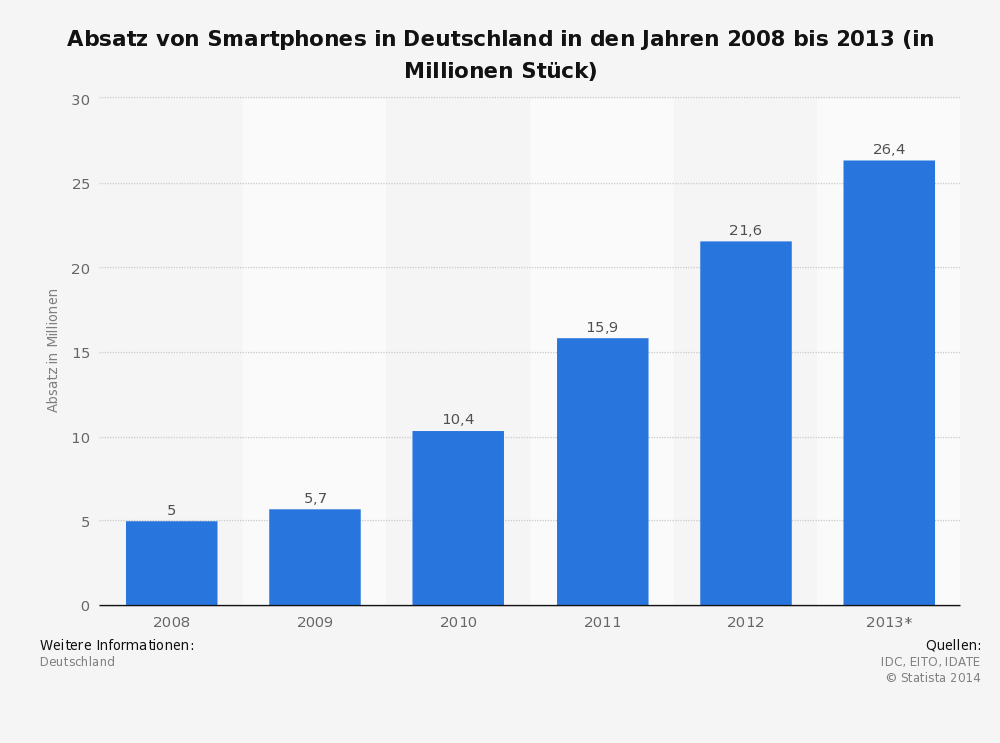
\includegraphics[height=8cm]{pictures/statistik-smartphonenutzung.png}
		\caption{Smartphoneabsatz in Deutschland}
\end{figure}

Für die Realisierung der Indoor Positionierung kommen verschiedene Technologien in Frage. Darunter zum Beispiel Wireless LAN, RFID oder Bluetooth.
Diese Technologien bieten sich an, da sie standardmäßig in vielen Smartphones integriert sind und so nicht der Zwang besteht ein neues Gerät oder eine Erweiterung zu kaufen.


Schlussendlich viel die Entscheidung der zu verwendenden Technologie auf Bluetooth, da dieses eine sehr hohe Verbreitung bietet und auch viele Vorteile mit sich bringt. Zum einen ermöglicht Bluetooth eine schnelle und einfache Einrichtung und zum anderen benötigen die Bluetooth-Sendestationen wenig Energie, sodass nicht zwingend einen Stromanschluss vorhanden sein muss, sondern auch einen Batteriebetrieb über mehrere Monate bis Jahre hinweg möglich ist.

Die Positionierung in Innenräumen mittels Bluetooth ist ein relativ neuer Ansatz, welcher jedoch seit der Präsentation von Bluetooth Low Energy und der Vorstellung der iBeacons-Technologie von Apple immer mehr an Aufmerksamkeit gewonnen hat. So setzt zum Beispiel Apple selbst die iBeacons-Technologie in ihren Geschäften ein, um dem Kunden gezielte Werbung zu den in der Nähe befindlichen Produkten zu bieten.

%%%%%%%%%%%%%%%%%%%%%%%%%%%%%%%%%%%%%%%%%%%%%%%%%%%%%%%%%%%%
\section{Ziele der Bachelorarbeit}
\label{sec:introduction:goal}
%%%%%%%%%%%%%%%%%%%%%%%%%%%%%%%%%%%%%%%%%%%%%%%%%%%%%%%%%%%%


Das Hauptziel dieser Arbeit ist es zu untersuchen, in wie weit sich Bluetooth Low Energy, beziehungsweise die darauf basierende iBeacons-Technologie, für eine akzeptable Indoor Positionierung eignen, um Endgeräte zum Beispiel in Verkaufsräumen zu orten und zu identifizieren.

Dabei soll bestimmt werden, welches Verfahren sich am Besten für die Positionierung in Innenräumen eignet und ob es Unterschiede zwischen verschiedenen Sende- und auch Empfangsgeräten gibt.

Für diese Tests werden ausschließlich Apple-Geräte genutzt, da hier eine übersichtlichere Auswahl auf dem Markt herrscht, sodass die Basis der zu nutzenden Geräte überschaubar bleibt und nur wenige Geräte getestet werden müssen. Ein weiterer Grund ist, dass iOS, das Betriebssystem des Apple iPhone und iPads, bisher das einzige mobile Betriebssystem ist, welches die iBeacons-Technologie offiziell und nativ unterstützt.

Im Laufe der Bachelorarbeit soll deshalb eine iOS-Applikation entwickelt werden, welche eine Positionierung in einem Innenraum implementiert. Dabei wird die von Apple bereitgestellte CoreLocation-API genutzt, welche die Verarbeitung der iBeacon-Daten übernimmt. Die genutzten iBeacon-Sender kommen von Drittherstellern und sind derzeit noch in einem Vorserienstadium. 

Zum Abschluss soll eine grundlegende Positionierung, eine Anzeige der aktuellen Position auf eine Karte und das Auslösen bestimmter Aktionen an festgelegten Orten implementiert sein.




\chapter{Technologien und Werkzeuge}
\label{chap:technologies}

%%%%%%%%%%%%%%%%%%%%%%%%%%%%%%%%%%%%%%%%%%%%%%%%%%%%%%%%%%%%
\section{Bluetooth 4.0}
\label{sec:technologies:bluetooth4}
%%%%%%%%%%%%%%%%%%%%%%%%%%%%%%%%%%%%%%%%%%%%%%%%%%%%%%%%%%%%

Der Bluetooth-Standard 4.0, auch Bluetooth Smart genannt, wurde am 30.Juni 2010 verabschiedet. Darin enthalten sind alle Protokolle der vorherigen Version 3.0, sowie Fehlerkorrekturen und Erweiterungen (\citet{bluetoothcore}). Außerdem wurde ein neues Protokoll hinzugefügt, Bluetooth Low Energy. 

Das erste unterstützte Mobilfunkgerät war das iPhone 4s (\citet{iphone4sspecs}), welches am 4. Oktober 2011 vorgestellt wurde. Im Jahr 2012 integrierten auch andere Smartphone-Hersteller Bluetooth 4.0 in ihre Geräte, sodass alle neueren Geräte diesen Standard beherschen.


%%%%%%%%%%%%%%%%%%%%%%%%%%%%%%%%%%%%%%%%%%%%%%%%%%%%%%%%%%%%
\subsection{Bluetooth Low Energy}
\label{sec:technologies:bluetoothLE}
%%%%%%%%%%%%%%%%%%%%%%%%%%%%%%%%%%%%%%%%%%%%%%%%%%%%%%%%%%%%

Bluetooth Low Energy wurde Anfangs von Nokia unter dem Namen ''Wibree'' entwickelt. Die Zielsetzung dabei war es eine Technologie zu entwickeln, mit der sich Computer und Mobilgeräte schnell und einfach mit Peripherie-Geräten verbinden lassen sollten. Das Hauptaugenmerk galt dabei dem geringen Stromverbrauch, einer kompakten Bauweise und den geringen Kosten der benötigten Hardware.
Im Jahr 2007 wurden diese Spezifikationen in den, sich in der Entwicklung befindlichen, Bluetooth-Standard 4.0 aufgenommen. Wibree wurde daraufhin in Bluetooth Low Energy, oder kurz BLE, umbenannt (\citet{wibree}).

Bluetooth Low Energy arbeitet wie das klassische Bluetooth im 2,4 GHz Band, bringt aber in der Funktionsweise einige Unterschiede mit sich.

So wurde, im Vergleich zum klassischem Bluetooth, die Datenrate von bis zu 3 Mbit/s auf maximal 1 Mbit/s reduziert. Dies führt dazu, dass BLE beispielsweise nicht für Headsets genutzt werden kann, da die zur Verfügung stehende Übertragungsrate nicht für eine Audioübertragung ausreicht.

Die Vorteile die BLE dabei mit sich bringt, liegen vor allem in der niedrigen Latenz, welche von 100ms auf weniger als 3ms reduziert wurde, und dem drastisch gesenkten Energieverbrauch im Vergleich zu den Vorgänger-Versionen. Der gesenkt Energieverbrauch hängt dabei mit verschiedenen Faktoren zusammen. 
Dabei wurde unteranderem die maximale Paketgröße auf 20 Byte verringert. Außerdem wurden die Empfangs- und Sendefenster verkleinert. 
Darüberhinaus arbeitet BLE nach dem Race-to-idle Prinzip. Dabei werden anstehende Daten schnellstmöglich gesendet und das Gerät geht, sobald die Daten verschickt worden sind, direkt in den Schlafmodus bis neue Daten vorliegen.

Eine weitere Neuerung ist die Nutzung einer 24-Bit-Fehlerkorrektur, welche die Verbindung unempfindlicher gegenüber Störungen und Übertragungsfehlern machen soll und so unnötige Neuübertragungen verhindert.

Auch die Verschlüsselung des zu übertragenden Signals wurde verbessert. Dabei kommt der Advance Encryption Standard (AES) mit einer Schlüssellänge von 128 Bit zum Einsatz (vgl. \citet{blespecs}). 

Das Bluetooth Low Energy Architektur besteht dabei aus verschiedenen Schichten und Komponenten (\citet{blespecsnordic}).

\textbf{Central und Peripheral}
Bei einer Bluetooth Low Energy-Verbindung unterscheidet man zwischen \emph{Central} und \emph{Peripheral}. Das Gerät in der Rolle des \emph{Central} horcht dabei auf gesendete Pakete von verbundenen oder allen in der Umgebung befindlichen Geräten. Das Gerät in der Rolle des \emph{Peripheral} hingegen sendet Pakete an die verbundenen oder an alle Geräte.


\textbf{ATT}
Das \emph{Attribute Protocol}, oder kurz \emph{ATT}, wird bei allen Datenübertragungen mittels Bluetooth Low Energy genutzt. Es wurde speziell für Bluetooth LE entworfen, um eine schnelle und sparsame Übertragung zu ermöglichen. 
Ein Attribut-Paket des ATT besteht dabei aus drei Bestandteilen. Einem 16 Bit \emph{Handle}, einem 128 Bit \emph{Universally Unique Identifier (UUID)} und einem \emph{Value} mit variabler Länge.
Der \emph{Handle} ist eine Nummer, welche das Attribut eindeutig identifiziert, da mehrere Attribute mit gleichem UUID möglich sind.
Der \emph{UUID} beschreibt den Typ des gesendeten Attributes, wobei die verschiedenen UUID's nicht im ATT festgelegt werden, sondern in darüberliegenden Profilen wie etwa GATT.
Die Länge des \emph{Value's} hängt dabei von dem Typ des gesendeten Attributes ab, lässt sich also in höheren Protokollen aus dem UUID bestimmen.

Das ATT basiert dabei auf einer Client-Server-Architektur, wobei nur der Server Attribute speichert und der Client diese ausliest oder schreibt.

\textbf{GATT}
Das \emph{Generic Attribute Profile (GATT)} ist verpflichtend für alle Bluetooth LE-Profile. Es basiert dabei auf ATT und erlaubt ein einfache und geregelte Übertragung der Attribute. Ein Beispiel für ein GATT-Profil ist das \emph{Heart Rate Profile}, welches für Herzfrequenzmessungen designt wurde.
Jedes Profil besteht dabei aus verschiedenen Attributen, welche hierarchisch aufgebaut sind.
Die einzelnen Attribut-Typen unterscheiden sich dabei durch ihre UUID, welche in den GATT-Profilen eindeutig festgelegt sind.

An oberster Stelle steht dabei das \emph{Service}-Attribut. Ein Service besteht aus einer Menge von \emph{Characteristics}. Eine Beispiel für einen GATT-Service ist der \emph{Heart Rate Service}, welcher aus mehreren \emph{Characteristics} besteht, wie zum Beispiel der \emph{Heart Rate Measurement Characteristic}, welche die aktuelle Herzfrequenz beschreibt oder der \emph{Body Sensor Location Characteristic}, welche die Lage des Herzfrequenzmessers beschreibt. 
Das \emph{Characteristic}-Attribut besteht aus einem Messwert und einem \emph{Descriptor}. Der aktuelle Wert ist abhängig von der Characteristic, so gibt die \emph{Heart Rate Measurement Characteristic} beispielsweise die aktuelle Herzfrequenz als Wert zurück. 
Der \emph{Descriptor} liefert zusätzliche Information über die aktuelle \emph{Characteristic}, wie zum Beispiel den erlaubten Wertebereich oder die Einheit in welcher der Messwert vorliegt.

\begin{figure}[htb!]
		\centering
	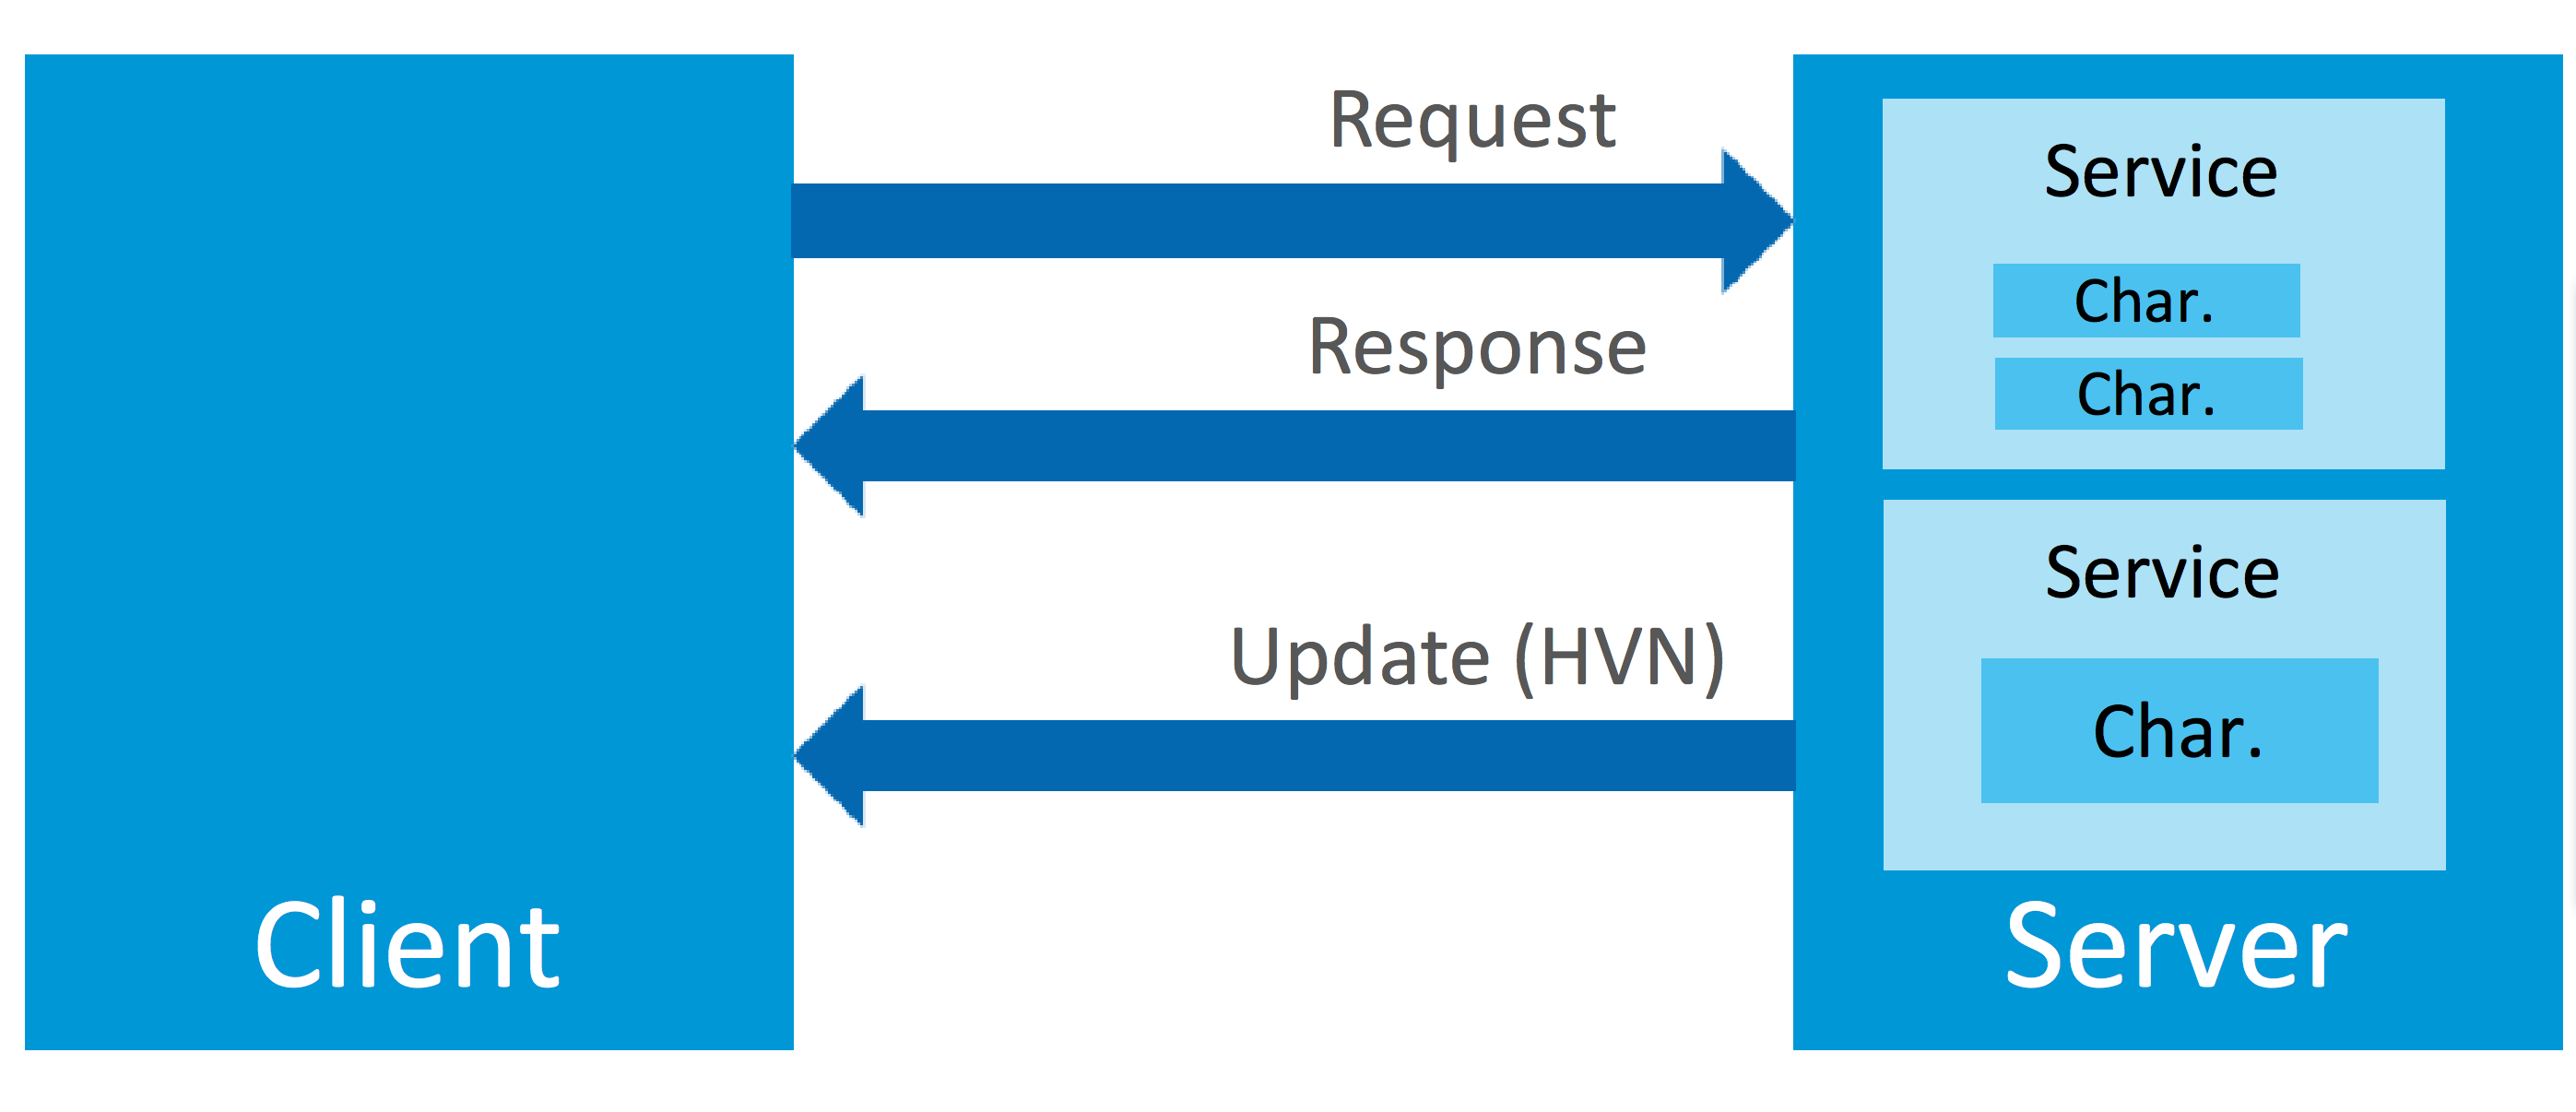
\includegraphics[scale=0.3]{nordic-gatt-overview}
	\caption{Verbindug zwischen Client und Server bei GATT-Übertragung}
	\label{nordic-gatt-overview}
	\end{figure}


%%%%%%%%%%%%%%%%%%%%%%%%%%%%%%%%%%%%%%%%%%%%%%%%%%%%%%%%%%%%
\subsection{iBeacons}
\label{sec:technologies:bluetoothLE:ibeacons}
%%%%%%%%%%%%%%%%%%%%%%%%%%%%%%%%%%%%%%%%%%%%%%%%%%%%%%%%%%%%
Die iBeacons-Technologie wurde am 10.Juni 2014 von Apple auf der Worldwide Developers Conference vorgestellt (\citet{appleinsideribeacons}). 
Diese basiert auf Bluetooth Low Energy und arbeitet mit einem von Apple entwickelten, proprietären GATT-Profil.

Beacon bedeutet übersetzt ''Leuchtfeuer'' und die Funktionsweise der Beacons ist dem sehr ähnlich.
Einmal in Betrieb genommen, sendet das Beacon dauerhaft, in kleinen Zeitintervallen, ein Signal in welchem sich Daten zur Identifizierung und Entfernungsbestimmung des Beacons befinden.

Für die Identifizierung sendet das Beacon drei Werte, den \emph{Universally Unique Identifier (UUID)}, den \emph{Major}-Wert und den \emph{Minor}-Wert.
Der \emph{UUID} ist ein Identifier, welcher Beacons einem bestimmten Typ oder einem Unternehmen zuordnen. Dieser UUID lässt sich mittels diversen Programmen generieren.

Der \emph{Major}-Wert dient zur Unterscheidung von Beacons mit dem selben UUID und wird dazu eingesetzt, verschiedene Standorte beziehungsweise Regionen zu unterscheiden. Ein Beispiel dafür wäre ein Unternehmen mit mehreren Standorten, sodass bei gleichem UUID eine eindeutige Bestimmung des Standortes möglich ist.

Der \emph{Minor}-Wert dient zur weiteren Unterscheidung der Beacons mit gleichem UUID und Major-Wert. Vorgesehen ist der Minor-Wert zur Bestimmung eines einzelnen Beacons in einer bestimmten Region, es ist jedoch nicht verboten mehreren Beacons die gleichen UUID, Major und Minor-Werte zu zuweisen, wodurch jedoch keine eindeutige Identifizierung mehr möglich ist. 

Neben den von Beacon gesendeten Identifikationsdaten kann das Empfangsgerät selbst noch weitere Größen bestimmen. Es ist so zum Beispiel möglich die ungefähre Entfernung zu erhalten. 
Dafür wir der \emph{Proximity}-Wert genutzt. Dieser definiert vier verschiedene Entfernungs-Zustände : \textit{Far(mehr als 10m)}, \textit{Near(wenige Meter)}, \textit{Immediate (wenige Zenitmeter)} und \textit{Unknown(Entfernung konnte nicht bestimmt werden)}. 
Diese Werte erlauben eine sehr grobe Entfernungseinschätzung zum Beacon. 
Für eine differenziertere Entfernungsbestimmung lässt sich eine weitere Kennzahl bestimmen, der \textit{Accuracy}-Wert. Dabei handelt es sich um eine ungefähre Entfernungsangabe in Metern, welche jedoch ausdrücklich nur zur Differenzierung der Enterfernung zweier Beacons genutzt werden soll und keinesfalls einen genauen Abstand zum Beacon angibt. Der Accuracy-Wert soll dabei erlauben, bei gleichem Proximity-Wert, das nächstgelegene Beacon zu bestimmen (\citet{clbeaconref}).

\begin{figure}[htb!]
		\centering
	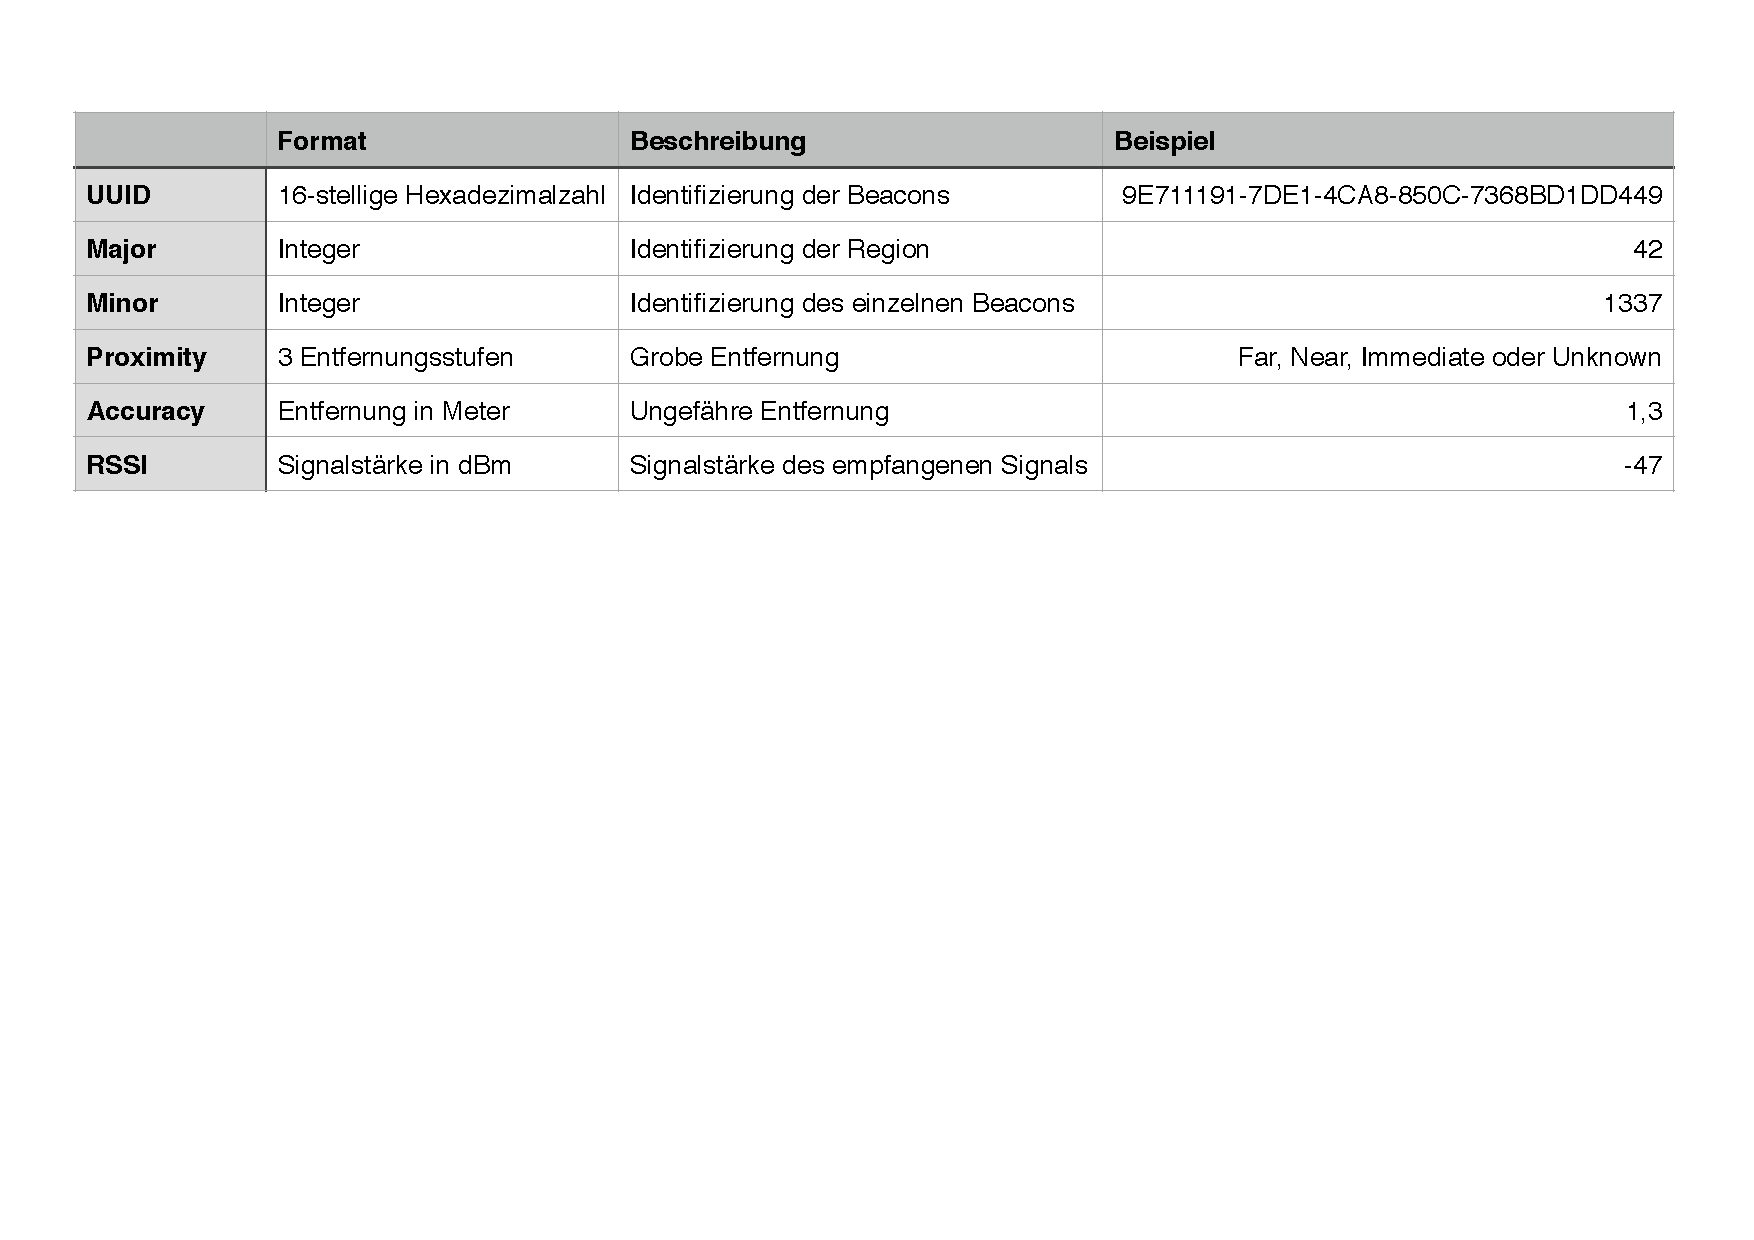
\includegraphics[scale=0.5]{ibeacon-table}
	\caption{Beacon-Daten beim Empfangsgerät}
	\label{ibeacon-table}
\end{figure}


Die von dem Beacon gesendeten Daten lassen sich mit jedem BLE-kompatiblem Gerät empfangen, bisher bietet jedoch nur iOS eine entsprechende, native Unterstützung für das iBeacon-Profil.

Die großen Vorteile der iBeacons sind ihr kleiner Formfaktor, welcher es erlaubt die Beacons an fast jedem beliebigem Ort anzubringen, und ihr geringer Stromverbrauch, der es möglich macht, die Beacons mit einer Knopfzellen-Batterie zu betreiben und das, laut Herstellerangaben, für bis zu zwei Jahre.
Der Aufbau eines solchen Beacons lässt sich in Abbildung \ref{estimote-beacon} erkennen. Den Großteil des Beacons nimmt dabei die Batterie ein. 


%%%%%%%%%%%%%%%%%%%%%%%%%%%%%%%%%%%%%%%%%%%%%%%%%%%%%%%%%%%%
% figure of estimote beacon
%%%%%%%%%%%%%%%%%%%%%%%%%%%%%%%%%%%%%%%%%%%%%%%%%%%%%%%%%%%%
\begin{figure}[h!]
	\centering
	\begin{minipage}[t]{5cm}
		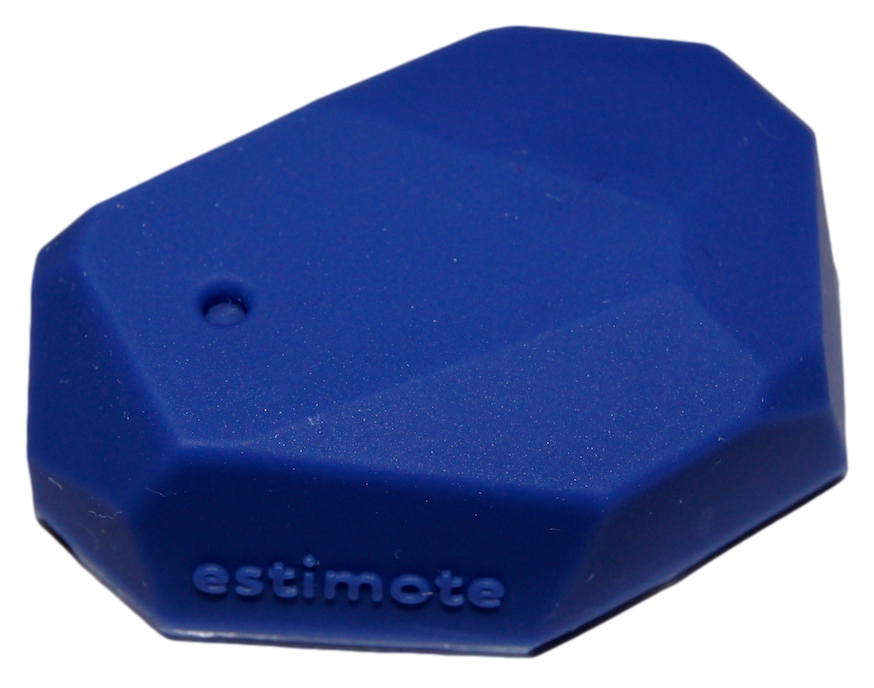
\includegraphics[scale=0.15]{pictures/estimote-beacon-outside}
		\caption{Außenhülle}
		\label{estimote-outside}
	\end{minipage}
	\hspace{2cm}
	\begin{minipage}[t]{5cm}
			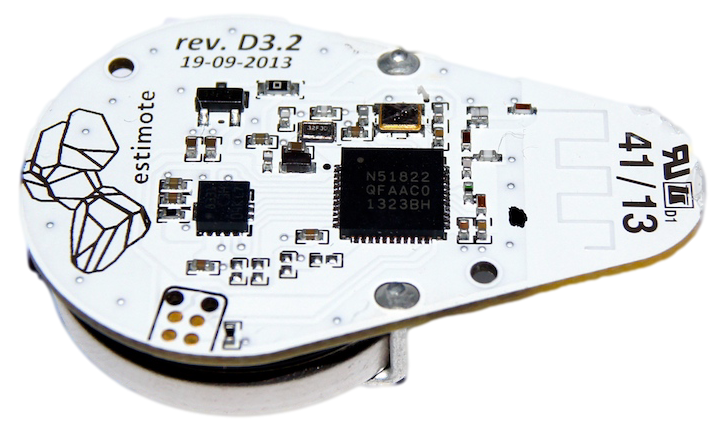
\includegraphics[scale=0.2]{pictures/estimote-beacon-inside}
			\caption{Chipsatz mit Bluetooth-Modul}
			\label{estimote-inside}
	\end{minipage}
		\caption{Ein iBeacon der Firma ''estimote''}
		\label{estimote-beacon}
\end{figure}


Unter genauerer Betrachtung der Platine in Abbildung \ref{estimote-beacon-inside-annotations}, erkennt man, dass diese im Grunde aus zwei Teilen besteht.
Dem Bluetooth-Chipsatz, welcher an sich ist nur wenige Zentimeter groß ist und der Antenne, welche im vorderen Bereich der Platine eingearbeitet ist und über die letztendlich die Daten gesendet werden.

\begin{figure}[h!]
	\centering
	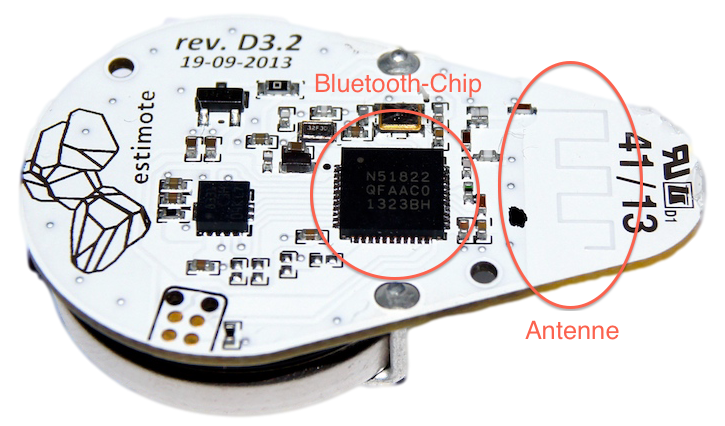
\includegraphics[scale=0.25]{estimote-beacon-inside-annotation}
	\caption{Aufbau des estimote-Beacons}
	\label{estimote-beacon-inside-annotations}
\end{figure}



%%%%%%%%%%%%%%%%%%%%%%%%%%%%%%%%%%%%%%%%%%%%%%%%%%%%%%%%%%%%
\section{Xcode}
\label{sec:tools:xcode}
%%%%%%%%%%%%%%%%%%%%%%%%%%%%%%%%%%%%%%%%%%%%%%%%%%%%%%%%%%%%
Xcode ist eine integrierte Entwicklungsumgebung, welche von Apple etwickelt wurde. Xcode ermöglicht es native \emph{iOS} und \emph{OS X} Applikationen zu erstellen, zu testen und zu debuggen.
Standardmäßig werden dabei die Programmiersprachen \emph{Objective C}, \emph{C} und \emph{C++} unterstützt.

Xcode stellt viele Features für die Programmierung bereit, wie zum Beispiel \emph{code completion}, vorgefertigte \emph{Templates}, einen umfangreichen \emph{Debugger} und eine \emph{iOS-Simulator} für das Testen der Applikationen, ohne diese auf ein reales Gerät zu übertragen (\citet{xcodeinfo}).


\textbf{Templates}

Xcode stellt verschiedene, vorgefertigte iOS-Templates zur Verfügung. 
Dabei bringt jedes Template eigene Funktionen mit sich. In Abbildung \ref{xcode-templates} lassen sich die verschiedenen Auswahlmöglichkeiten erkennen.

\begin{figure}[htb!]
		\centering
	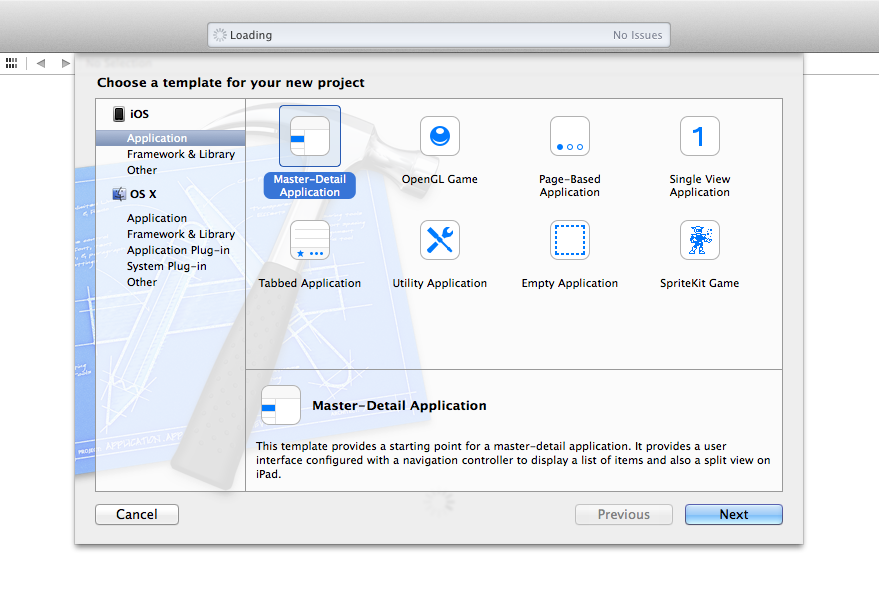
\includegraphics[scale=0.4]{xcode-templates}
	\caption{Auswahlbildschirm der verschiedenen Templates}
	\label{xcode-templates}
\end{figure}

Nach der Auswahl des Templates, werden die dem Template entsprechenden Dateien im Dateiexplorer angelegt.


Dazu gehören beispielsweise die \emph{AppDelegate} und die \emph{Storyboards}.

Die AppDelegate-Klasse steuert applikationsweite Ereignisse, wie etwa das Aufrufen und Schließen der Applikation. Außerdem wird durch die AppDelegate der aktuelle Zustand der Applikation gespeichert und bei Bedarf wiederhergestellt.


\textbf{Interface Builder}

Der Interface Builder ist ein in Xcode integrierter, grafischer Editor, welcher es erlaubt die Benutzeroberflächer einer iOS-Applikation zu erstellen. Dabei werden Storyboards genutzt.
Ein Storyboard ist die Repräsentation der grafischen Oberfläche einer Applikation und besteht dabei aus einem oder mehreren Views.

Die Views lassen sich nach dem \emph{Drag and Drop}-Prinzip zusammenstellen. Dabei stehen weitere Inteface-Elemente, wie zum Beispiel Textfelder, Buttons oder Schalter, zur Verfügung.

\begin{figure}[htb!]
	\centering
	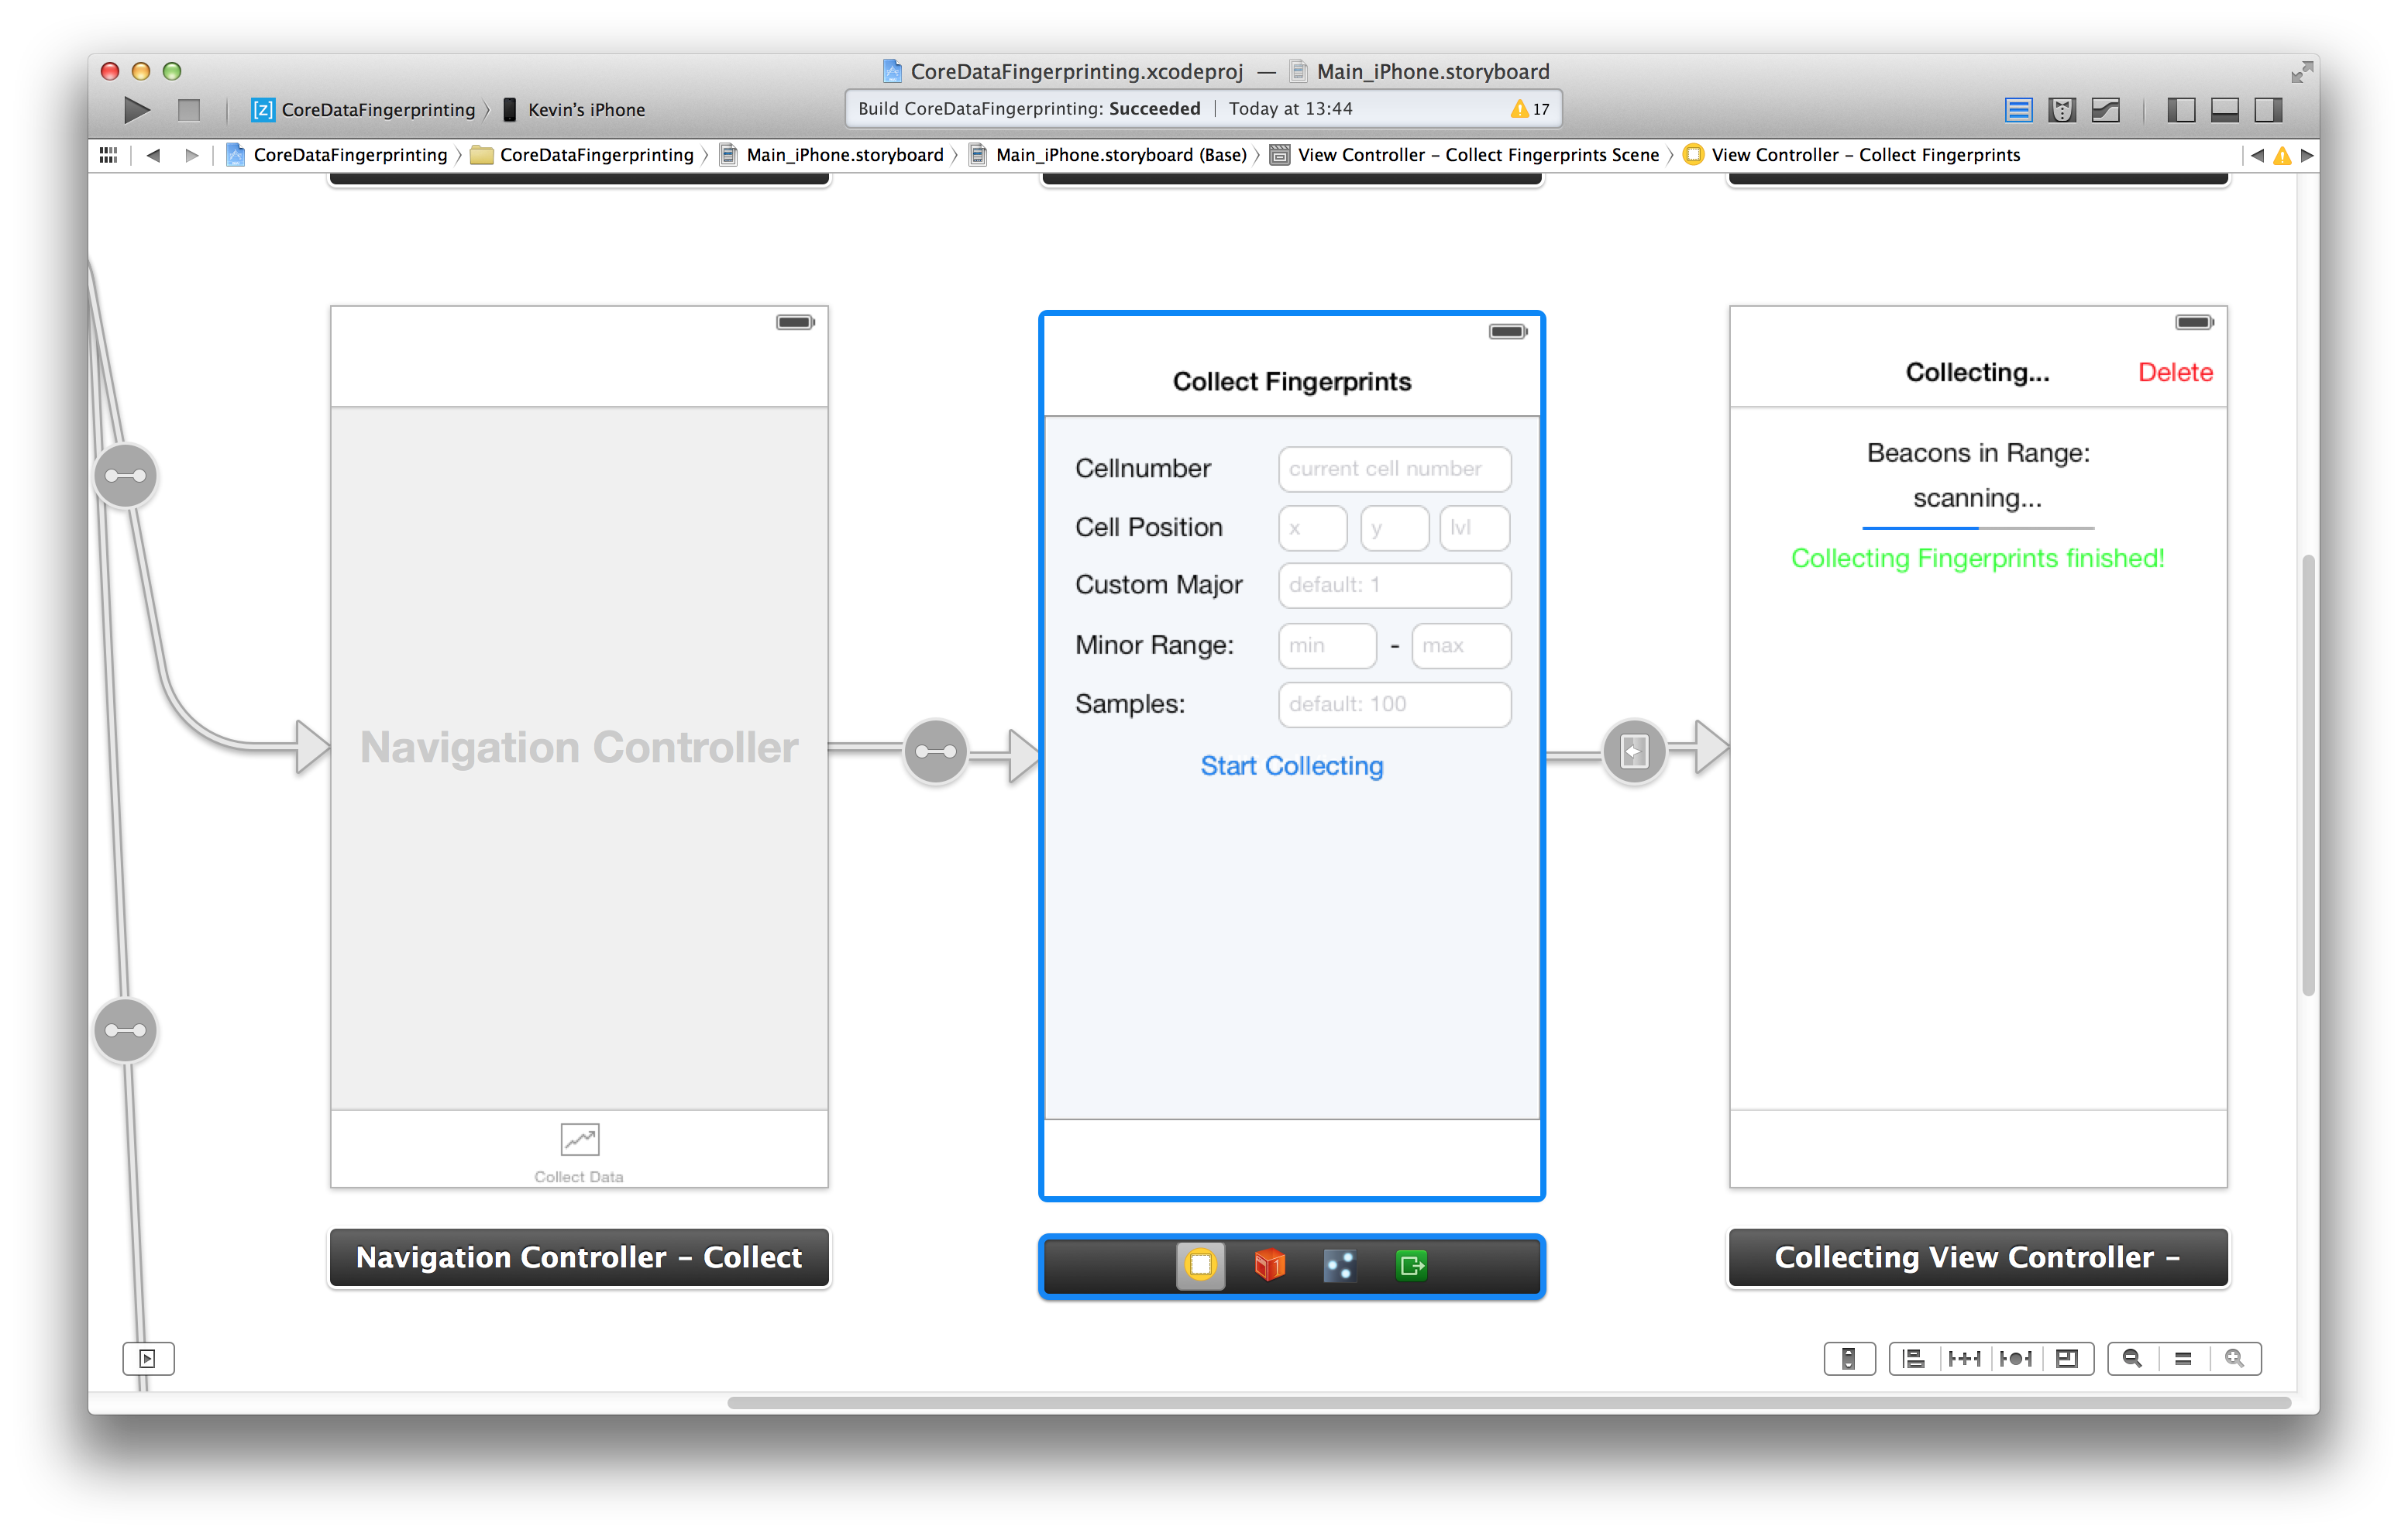
\includegraphics[scale=0.25]{xcode-storyboard}
	\caption{Interface Builder für eine iPhone-Applikation}
	\label{xcode-interface-builder}
\end{figure}

Wie in Abbildung \ref{xcode-interface-builder} zu erkennen, besteht das Storyboard aus mehreren Views, die jeweils eine gezeigte Szene auf dem Gerät repräsentieren. Die einzelnen Views sind mit \emph{Segue's} verbunden. Ein Segue, auf deutsch Übergang, steuert dabei den Wechsel zwischen den Views. Dabei wird zum Beispiel festgelegt durch welche Aktion dieser ausgelöst wird und wie dieser abläuft.


Der Interface Builder bietet außerdem noch die Funktion des \emph{Auto Layout}. Dabei werden sogenannte \emph{Constraints} genutzt, welche die Positionsbeziehungen zwischen den einzelnen Elementen des Views festlegen. Diese Constraints erzeugen so ein dynamisches Interface, welches sich an das verwendete Gerät anpasst und so ein User Interface, unabhängig der Bildschirmgröße oder der aktuellen Orientierung des Bildschirms, darstellt. (\citet{xcodeautolayout})

\begin{figure}[htb!]
		\centering
	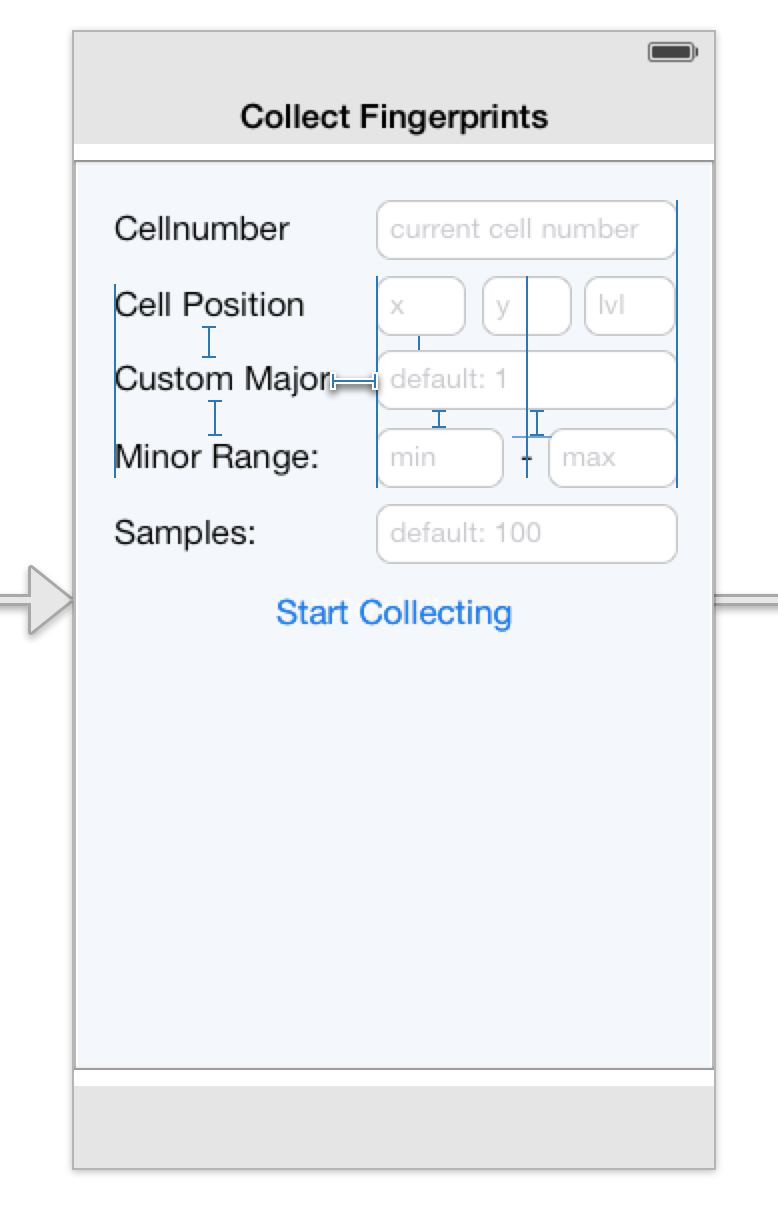
\includegraphics[scale=0.5]{xcode-storyboard-constraints}
	\caption{View Controller mit Constraints}
	\label{xcode-storyboard-constraints}
\end{figure}

Diese Constraints beschreiben dabei die Abstände und Ausrichtungen der einzelnen Elemente zu dem umschließenden View oder den Elementen innerhalb des Views.

Eine iOS-Applikation kann über mehrere Storyboards verfügen, wodurch es möglich ist, die gleiche Applikation sowohl für das iPhone als auch das iPad anzupassen.


\textbf{iOS Simulator}

Für das Testen und Debuggen der Applikation bringt Xcode einen iOS-Simulator mit sich. Dieser erlaubt das Ausführen einer Applikation auch ohne ein iPhone oder iPad. Der Simulator bietet dabei verschiedene Konfigurationen, sowohl für iPhone (3,5 Zoll und 4 Zoll) als auch für das iPad (retina und non-retina).
Im Bezug auf Bluetooth bietet der Simulator jedoch keine entsprechende Unterstützung (\citet{iossimulator}).

%%%%%%%%%%%%%%%%%%%%%%%%%%%%%%%%%%%%%%%%%%%%%%%%%%%%%%%%%%%%
\section{iOS}
\label{sec:technologies:iosandxcode}
%%%%%%%%%%%%%%%%%%%%%%%%%%%%%%%%%%%%%%%%%%%%%%%%%%%%%%%%%%%%
Für die Entwicklung der Applikation zur Indoor Positionierung war eine der Vorgaben, dass diese für iOS programmiert werden soll.
Apple hat dabei für die iOS Programmierung verschiedene Vorraussetzungen. Zum einen benötgt man einen Mac, da nur hier die benötigte Software installiert werden kann.
Dazu zählt in erster Linie Xcode, welches als Entwicklungsumgebung für iOS-Applikationen genutzt wird (\citet{iossetup}). 
Außerdem wird ein iOS-Gerät vorrausgesetzt, da, wie bereits erwähnt, der iOS-Simulator kein Unterstützung für Bluetooth mit sich bringt. 
Die eingesetzten iOS-Gerät sind ein iPhone 5 und ein iPhone 4s. Auf beiden Geräten ist die aktuelle iOS-Version 7.1 installiert.

Die vorrausgesetzte, minimale iOS-Version ist dabei iOS 7, da die iBeacon-API des CoreLocation-Frameworks (mehr dazu im Kapitel \ref{sec:technologies:corelocation}) erst ab dieser Version zur Verfügung stehen.

%%%%%%%%%%%%%%%%%%%%%%%%%%%%%%%%%%%%%%%%%%%%%%%%%%%%%%%%%%%%
\textbf{iOS Developer Program}
Um eine programmierte Anwendung letztendlich auf einem iOS-Gerät auszuführen, ist die Mitgliedschaft im iOS Developer Program notwendig.
Diese erlaubt das Testen der Anwendung auf dem Gerät, die Veröffentlichung im AppStore und gewährt Zugriff auf das iOS Beta-Programm, um Anwendungen für neue Versionen des Betriebssystems zu optimieren.
Die Mitgliedschaft in diesem \emph{iOS Developer Program} kostet jährlich 99 Dollar (\citet{iosdevprog}). 
Im Rahmen meine Bachelorarbeit wurde der Zugang zu diesem Programm von der Universität zur Verfügung gestellt. Dabei beschränkt sich der Funktionsumfang jedoch auf das Testen der Applikation auf dem Gerät, da die Veröffentlichung im AppStore und der iOS Beta-Programm nicht teil des Pakets für Universitäten ist.

\textbf{iPhone}
Für die Entwicklung und das Testen der Applikation wurde ein iPhone 5 und ein iPhone 4s verwendet. 
Hauptsächlich wurde das iPhone 5 genutzt, wobei das iPhone 4s als Vergleichsgerät diente, um Messwerte zu vergleichen oder zu überprüfen.

Das Ausführen der geplanten Applikation auf einem realen Endgerät ist dabei unverzichtbar, da der iOS-Simulator nicht die Möglichkeit besitzt Bluetooth-Signale zu empfangen.

Das iPhone 4s wurde dazu genutzt, zu überprüfen in wie weit die Ergebnisse der Messwert zwischen einzelnen Geräten übertragbar sind, beziehungsweise wie sich diese zwischen einzelnen Modellgenerationen unterscheiden, da diese verschiedene Hardware einsetzen. 

So setzt das iPhone 4s auf den Broadcom BCM4330-Chipsatz, welches ein Wireless LAN-Chip mit integriertem Bluetooth 4.0 ist (\citet{iPhone4sTeardown}). Das iPhone 5 dagegen setzt auf den BCM4334 (\citet{iPhone5Teardown}), ebenfalls von Broadcom. 
Auch der Aufbau der Antennen und das Material der iPhones unterscheidet sich zwischen diesen beiden Generationen deutlich. 
So ist das iPhone 4s mit einer Glas-Rückseite ausgestattet, wohingegen das iPhone 5 einen Rückseite aus Aluminium besitzt.

Daher ist es wichtig zu vergleichen, in wie weit diese Unterschiede Einfluss auf die Empfangsqualität haben und zu bestimmen, ob eine Übertragung der Messwerte zwischen den Geräten möglich ist oder jedes Gerät individuell behandelt werden muss.

\begin{figure}[htb!]
		\centering
	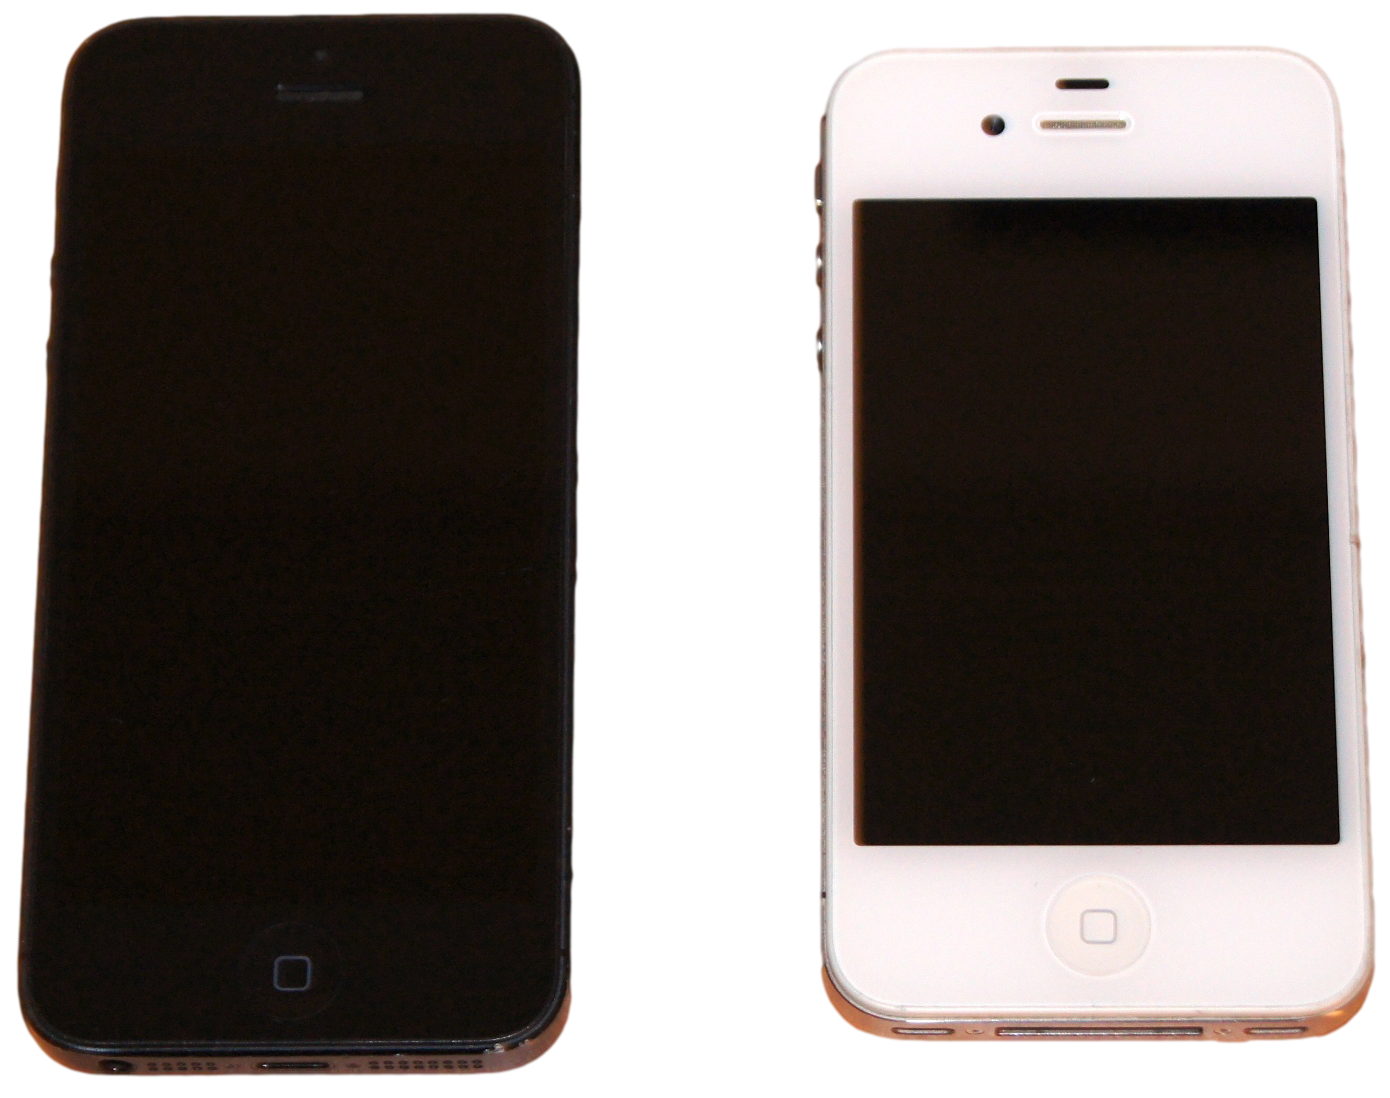
\includegraphics[scale=0.1]{iphones}
	\caption{Die für die Messungen und Tests genutzten iPhones}
	\label{iphones}
\end{figure}

\textbf{Objective-C}
Für die Implementierung der Applikation kam als Programmiersprache \emph{Objective-C} zum Einsatz, welches die primäre Sprache zur Programmierung von iOS-Anwendugen ist. 
Diese bietet viele nützliche Eigenschaften, wie etwa dynamisches Binden, eine dynamische Typisierung oder \emph{Fast Enumeration}.
Im Vergleich zu Java arbeitet \emph{Objective-C} nicht mit Methodenaufrufen, sondern mit Nachrichten. Diese werden von einem Sender zu einem Empfänger gesendet, wobei der Empfänger daraufhin entscheidet, was geschieht beziehungsweise welche Methode ausgeführt wird. Ein weitere Besonderheit von Objective-C sind die Properties (Eigenschaften), welche den Instanzvariablen entsprechen, jedoch noch weitere Konfigurationsmöglichkeiten hinsichtlich Schreibschutz und Atomarität bieten.
Eine weiterer Unterschied ist die Syntax von Objective-C.

\begin{listing}[htb!]
    \insertminted{objc}{code_examples/helloworld.m}
    \caption{Hello World-Beispiel in Objective-C und Java}
	\label{lst:helloworld_objc}
\end{listing}

Der Hauptunterschied liegt in der Methodendeklaration. Statt des \emph{static} Schlüsselwortes wird bei Objective-C eine Klassenmethode mit einem ''+'' gekennzeichnet. Eine Instanzmethode wird mit einem ''-'' deklariert. Der nächste Unterschied wird bei den Übergabewerten deutlich. Diese werden bei Objective-C, mit einem '':'' abgetrennt, angegeben.
Ein weiterer Unterschied wird beim Aufruf der Methoden deutlich. Da Objective-C nicht explizit die Methode aufruft, sondern eine Nachricht an die Klasse sendet, unterscheidet sich die Syntax deutlich. So werden hier eckige Klammern genutzt, wobei der Empfänger der Nachricht zuerst aufgeführt wird und danach die zu sendende Nachricht eingefügt wird (\citet{objc}).


%%%%%%%%%%%%%%%%%%%%%%%%%%%%%%%%%%%%%%%%%%%%%%%%%%%%%%%%%%%%
\section{CoreLocation-Framework}
\label{sec:technologies:corelocation}
%%%%%%%%%%%%%%%%%%%%%%%%%%%%%%%%%%%%%%%%%%%%%%%%%%%%%%%%%%%%
Das CoreLocation-Framework ist ein iOS-Framework, welches es erlaubt die aktuellen Positions- und Richtungsinformationen eines Gerätes zu bestimmen und auszugeben.
Die Positionsbestimmung lässt sich dabei über verschiedene Sensoren und Werte bestimmen, wobei der Grad der Genauigkeit variabel ist.
Für die Positionsbestimmung lässt sich zum Beispiel das integrierte GPS-Modul verwenden.
Auch die Aktualisierungsrate der Position lässt sich festlegen, wobei eine höhere Aktualisierungsrate und eine höhere Genauigkeit auch gleichbedeutend mit einem höherem Akkuverbrauch sind.
	
Die Genauigkeit lässt sich dabei nur bei der Positionierung mittels GPS einstellen und ist daher für die Indoor Positionierung nur bedingt geeignet. Es wäre jedoch denkbar, die Positionierung mittels GPS und die Positionierung mittels iBeacons zu verbinden und nahtlos in einander übergehen zu lassen.

Eine weitere Funktion des CoreLocation-Frameworks ist der Kompass, also die Bestimmung der Himmelsrichtungen. Durch den eingebauten Kompass in den neueren iOS-Geräten ist es möglich, die aktuelle Ausrichtung des Gerätes sehr genau zu bestimmen. Dies ist im Bezug auf die Indoor Navigation hilfreich, da diese Informationen in die Positionsbestimmung einbezogen werden können. Da der menschliche Körper die Signale der Beacons beeinflusst, ist es daher von Vorteil die aktuelle Ausrichtung zu kennen. Dadurch kann die aktuelle Position des Körpers bestimmt werden und in den Messungen berücksichtigt werden.

Des Weiteren erlaubt diese Funktion eine dynamische Anpassung der Karte, abhängig davon wie das Gerät aktuell ausgerichtet ist.

Die für uns zentrale Funktion dieses Frameworks ist die Erkennung von iBeacons und die Funktionen zur Verarbeitung der von den Beacons gesendeten Daten.
Mittels des Frameworks können Beacons anhand ihres UUID erkannt und einer Region zugeordnet werden. Die genaue Funktionsweise wird dabei im folgenden Kapitel behandelt. (\citet{corelocation})

%%%%%%%%%%%%%%%%%%%%%%%%%%%%%%%%%%%%%%%%%%%%%%%%%%%%%%%%%%%%
\subsection{iBeacons-API}
\label{sec:technologies:corelocation:ibeaconsapi}
%%%%%%%%%%%%%%%%%%%%%%%%%%%%%%%%%%%%%%%%%%%%%%%%%%%%%%%%%%%%
Mit der iOS Version 7 wurde das CoreLocation Framework um die Beacon-Funktionalitäten erweitert. 
Dazu wurden zwei neue Klassen hinzugefügt und das bestehende Framework dementsprechend angepasst. 
Hinzugefügt wurde zum einen die \emph{CLBeacon}-Klasse (\citet{clbeaconref}), welche ein iBeacon repräsentiert und alle zur verfügungsteheneden Informationen enthält und zum anderen die \emph{CLBeaconRegion}-Klasse (\citet{clbeaconregionref}), welche eine Region mit mehreren Beacons, abhängig von ihrem UUID und weiteren Werten, beschreibt.

Die \emph{CLBeacon}-Klasse besteht dabei lediglich aus Properties mit den gegebenen Beacon-Informationen, wie \emph{UUID}, \emph{major}, \emph{minor}, \emph{accuracy}, \emph{proximity} und \emph{rssi}.

Die \emph{CLBeaconRegion}-Klasse ist etwas umfangreicher und bestimmt letztendlich, nach welchen Beacons gesucht werden soll.
Dabei ist es möglich die Region in verschiedene Genaugikeits-Stufen zu initialisieren:


\emph{initWithProximityUUID:identifier:}\begin{quote}
	Die Region ist nur abhängig von dem UUID und dem Identifier der Beacons, das heißt es werden alle Beacons mit dem gegebenen UUID gesucht.
\end{quote}
\emph{initWithProximityUUID:major:identifier:}\begin{quote}
	Die Region ist abhängig von dem UUID, dem Identifier und dem Major-Wert der Beacons. Es werden nur Beacons eines bestimmten Major-Wertes gesucht.
\end{quote}
\emph{initWithProximityUUID:major:minor:identifier:}\begin{quote}
	Die Region ist abhängig von dem UUID, dem Identifier, dem Major-Wert und dem Minor-Wert der Beacons. Es werden nur Beacons mit passendem Major und Minor-Wert gesucht. In diesem Fall ist bei mehreren erkannten Beacons keine Unterscheidung mehr möglich.
\end{quote}

Die Beacon-Region bestimmt also letztlich nach welchen Beacons gesucht wird, beziehungsweise welche Beacons gefunden werden.

%%%%%%%%%%%%%%%%%%%%%%%%%%%%%%%%%%%%%%%%%%%%%%%%%%%%%%%%%%%%
\section{MapBox}
\label{sec:sec:technologies:mapbox}
%%%%%%%%%%%%%%%%%%%%%%%%%%%%%%%%%%%%%%%%%%%%%%%%%%%%%%%%%%%%
MapBox ist ein Online-Landkarten Anbieter, welcher es erlaubt eigene Karten zu erstellen und über ihren Service online bereitzustellen (\citet{mapboxweb}). 
Die Grundkarten werden dabei aus dem OpenStreetMap-Projekt entnommen und Mapbox erlaubt es diese Karten grafisch zu überarbeiten, um so zum Beispiel das Farbschema zu ändern, eigene Markierungen hinzuzufügen oder auch eigene Layer über die Karte zu legen.

Außerdem stellt Mapbox ein SDK (\citet{mapboxsdk})für iOS bereit, welche es erlaubt diese individuell angepassten Karten in iOS anzuzeigen und gleichzeitig die Funktionen des native MapKit-Framework, wie zum Beispiel Pinch-to-Zoom, automatische Kompassausrichtung oder Annotationen auf der Karte, mit sich bringt. Zudem besitzt Mapbox eine größere Flexibilität im Bezug auf die individuelle Anpassung der Karten und den Offline-Betrieb, als das von Apple für iOS bereitgestellte MapKit-Framework. Das Mapbox-SDK erlaubt es zum Beispiel die Karten direkt auf dem Gerät zu speichern.

Bisher ist die Unterstützung von Indoor-Karten jedoch noch nicht gegeben, sodass hierbei nicht auf vorhandenes Kartenmaterial zurückgegriffen werden kann, sondern eigenes Kartenmaterial bereitstellen muss.

Google hat mit \emph{Google Maps Indoor} bereits einen Dienst gestartet, welcher Gebäudepläne in Google Maps integriert (siehe \citet{googleindoormaps}). Dabei handelt es sich bisher jedoch hauptsächlich um öffentliche Gebäude in US-amerikanischen Städten. In Deutschland ist der Dienst ebenfalls schon gestartet, beinhaltet jedoch nur wenige Gebäude. Das Hinzufügen von neuen Gebäudeplänen ist nur bei öffentlichen Gebäuden möglich und nicht für den privaten Gebrauch vorgesehen, daher konnte nicht auf diesen Dienst zurückgegriffen werden.

Die Indoor-Karten mussten daher individuell für den Einsatzort erstellt und in ein, von Mapbox verständliches Format, umgewandelt werden.
Die Ausgangsdatei ist dabei eine Bilddatei in JPEG-Format, welches eine Karte des Innenraumes zeigt. Dieses Datei muss zur weiteren Verwendung in ein von Mapbox verständliches Format umgewandelt werden. 
Dazu wurde ein von ''Tom MacWright'' (\citet{jpgtogeo}) bereitgestellte Python-Script verwendet, welches JPEG Dateien in GeoTIFF Dateien umwandelt. Die GeoTIFF-Datei (\citet{geotiff}) speichert neben den eigentlichen Bildinformationen zusätzlich Koordinaten für die Georeferenzierung. 

Mit dieser GeoTIFF-Datei ist es nun möglich eine eigene Karte zu erstellen, welche letztendlich auf dem iOS-Gerät ausgegeben wird.
Dafür stellt Mapbox das Programm \emph{TileMill} zur Verfügung (\citet{tilemill}). Dieses erlaubt es eigene Karten zu erstellen und zu bearbeitet. Die erstellte Karte kann anschließend in verschiedenen Formaten exportiert werden. 
TileMill bietet einen Import von GeoTIFF-Dateien an, sodass unsere Karte direkt eingefügt werden kann.

\begin{figure}[htb!]
	\centering
	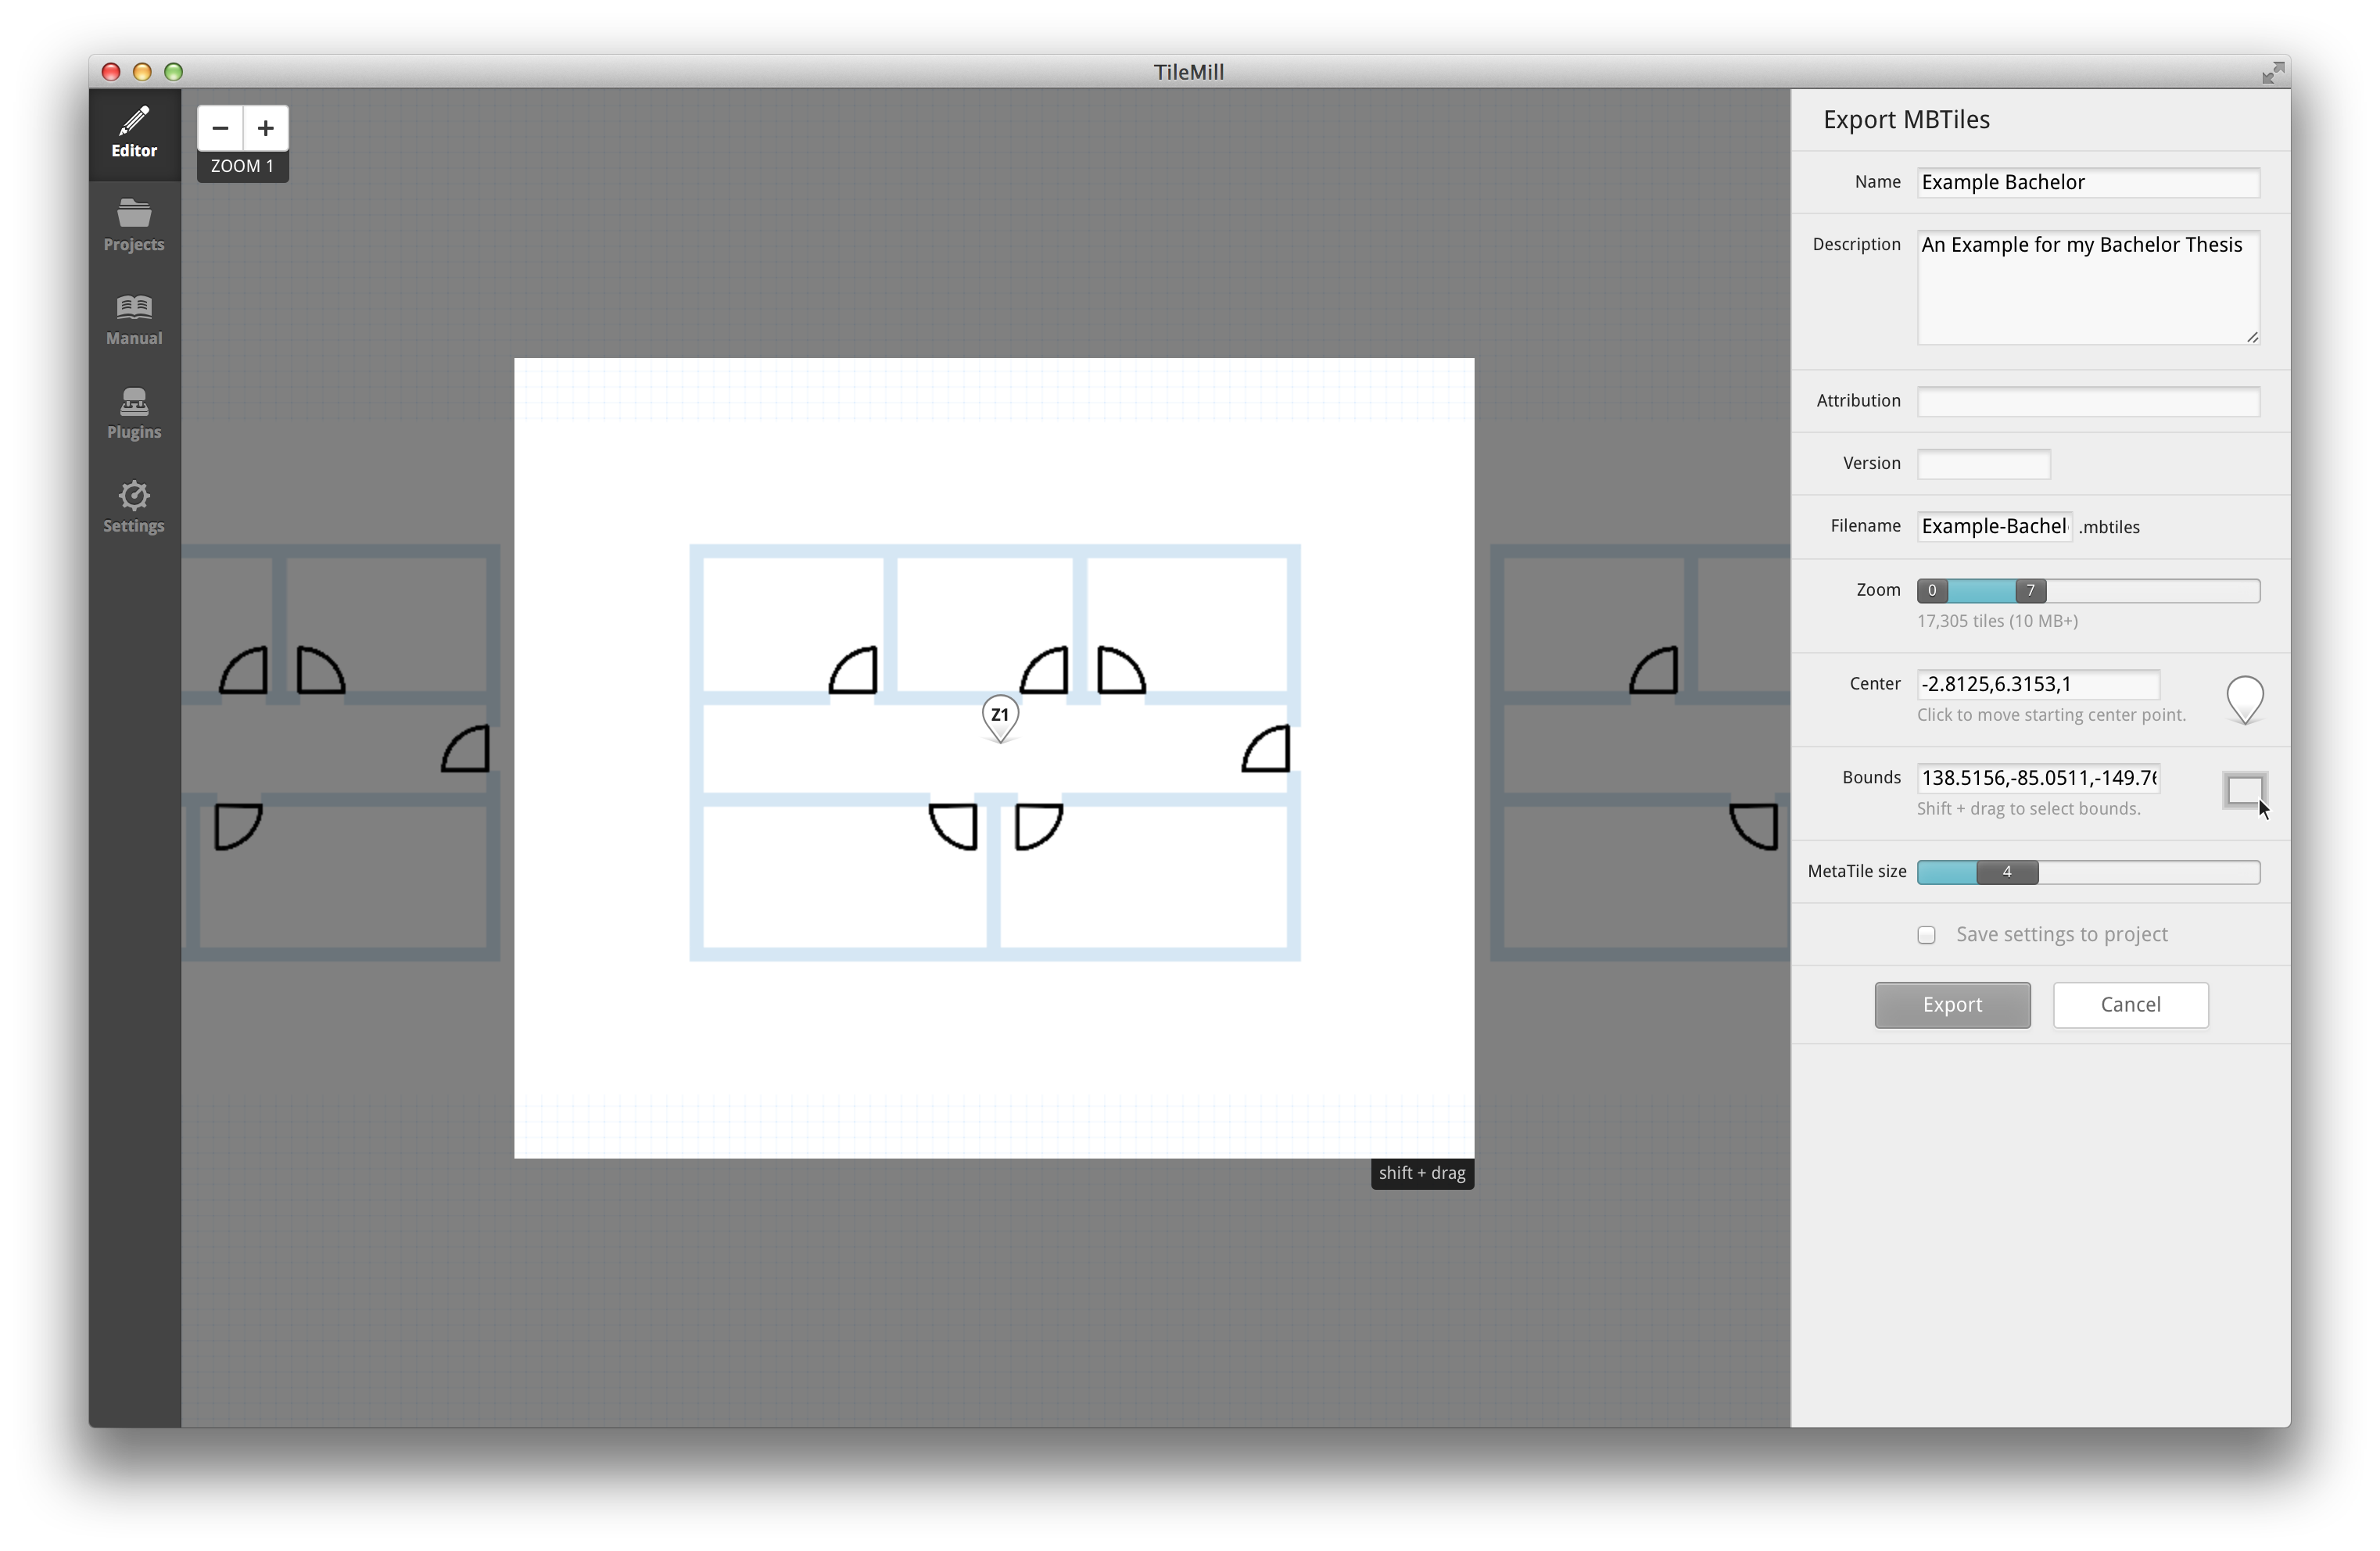
\includegraphics[scale=0.25]{tilemill-example}
	\caption{Karte in TileMill}
	\label{tilemill-example}
\end{figure}

TileMill erlaubt es nun die eingefügte Karte weiter zu bearbeiten oder Informationen hinzuzufügen.
Der nächste Schritt ist es die Karte in ein für iOS beziehungsweise das Mapbox SDK, verständliches Format zu überführen.
Dazu wird die Karte im \emph{mbtiles}-Format exportiert. Dies ist ein von Mapbox entwickeltes Dateiformat, welches die Karte in einzelne Kacheln überführt und speichert. Dadurch wird das Laden der einzelnen Kartenabschnitte bei größeren Karten beschleunigt, da nicht die komplette Karte geladen werden muss, sondern nur die aktuell benötigten Kacheln.

Die erzeugte \emph{.mbtiles}-Datei lässt sich nun in die iOS Applikation einbinden und über das SDK auf dem iOS-Gerät ausgeben. In Abbildung \ref{mapbox-map-ios} sieht man die Ausgabe einer Karte auf dem iPhone 5.

\begin{figure}[htb!]
		\centering
	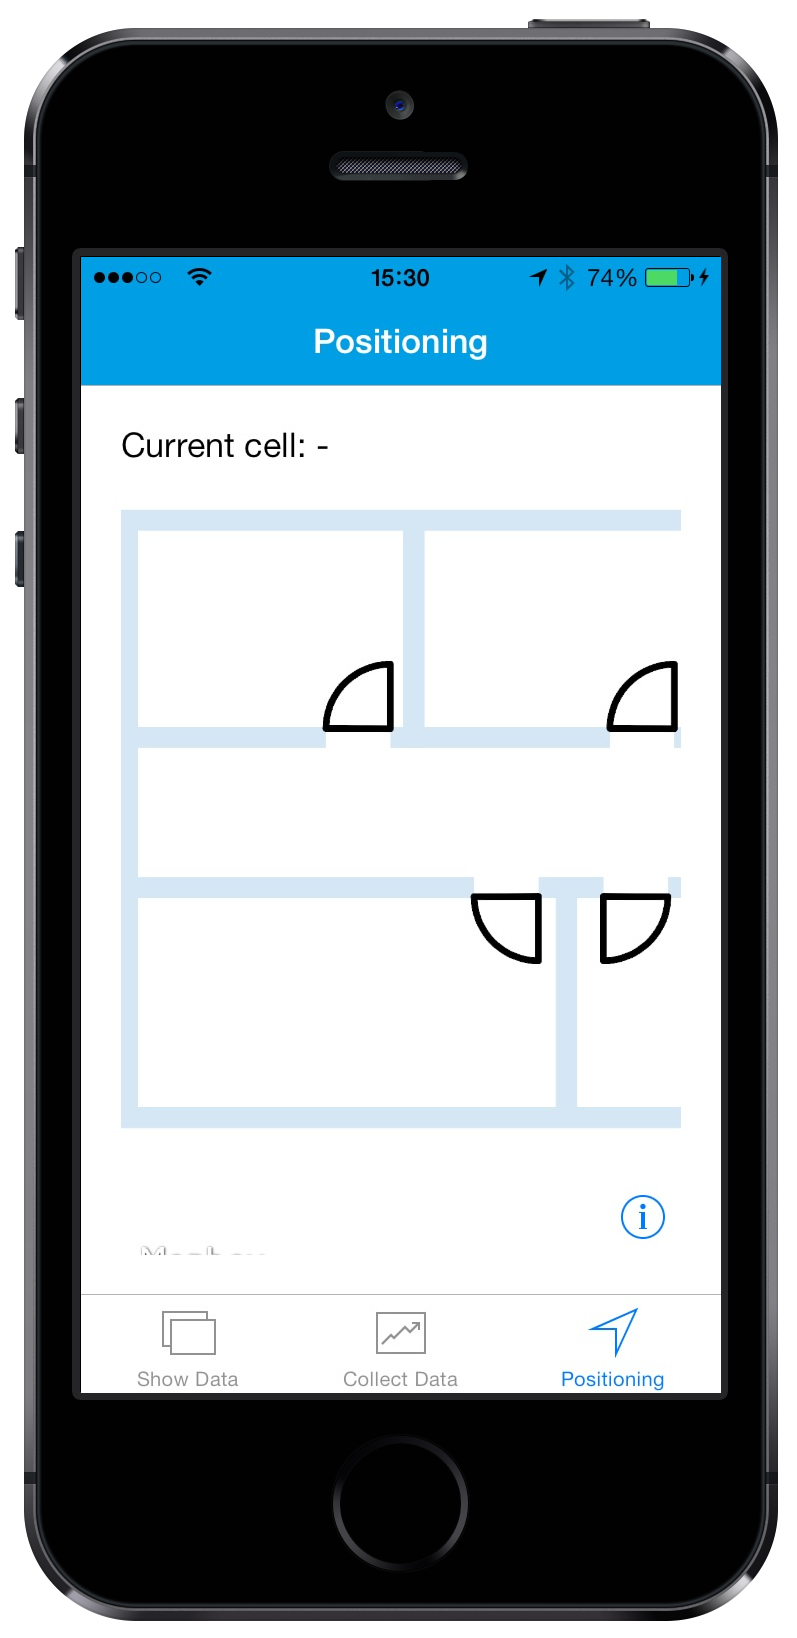
\includegraphics[scale=0.25]{mapbox-map-ios-mockup}
	\caption{Kartenausgabe mittels Mapbox SDK auf dem iPhone}
	\label{mapbox-map-ios}
\end{figure}

Diese Karte wird offline auf dem Gerät gespeichert, sodass keine Internetverbindung für die Anzeige nötig ist.

%%%%%%%%%%%%%%%%%%%%%%%%%%%%%%%%%%%%%%%%%%%%%%%%%%%%%%%%%%%%
\section{CoreData-Framework}
\label{sec:technologies:coredata}
%%%%%%%%%%%%%%%%%%%%%%%%%%%%%%%%%%%%%%%%%%%%%%%%%%%%%%%%%%%%
Das CoreData-Framework erlaubt die Verwaltung von Datenobjekten und deren Speicherung auf dem Gerät.
Dabei kommt ein relationales Datenmodell zum Einsatz, welches sich mittels grafischer Oberfläche in Xcode erstellen lässt.
In dem Modell lassen sich sowohl die Entitäten und ihre Attribute einstellen, als auch die Beziehungen zwischen den Entitäten definieren.
Die eigentliche Datenspeicherung sieht dabei drei verschiedene Speichermöglichkeiten vor: als Binärdatei, als XML-Datei oder in einer SQLite-Datenbank. 

Für die Erstellung eines CoreData-Modells bietet Xcode einen eigenen Editor an, welcher es erlaubt, Entitäten zum Modell hinzuzufügen und deren Attribute anzupassen. Die Beziehungen der Entitäten lassen sich dort ebenfalls erstellen und bearbeiten. Das Modell lässt sich dabei sowohl grafisch als auch in Tabellenform anzeigen.

\begin{figure}[htb!]
		\centering
	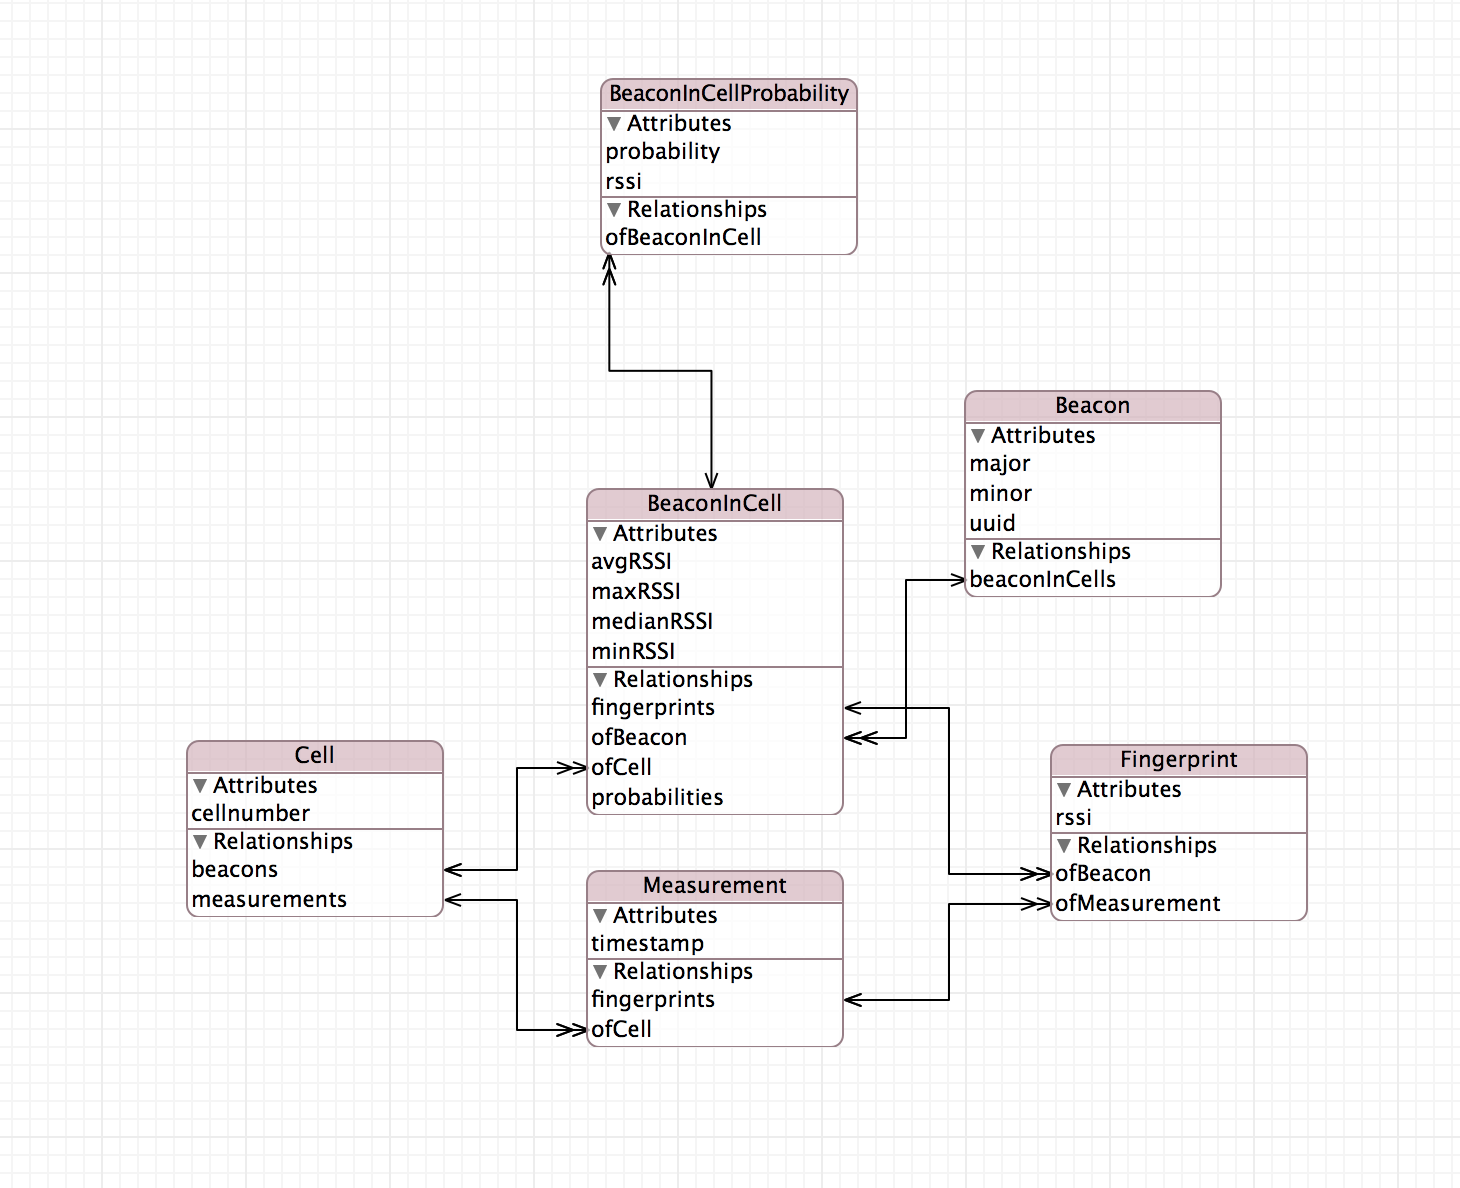
\includegraphics[scale=0.5]{coredata-model}
	\caption{CoreData-Modell in der grafischen Darstellung.}
	\label{coredata-model}
\end{figure}


Nachdem ein CoreData-Modell konfiguriert wurde, benötigt man für den Zugriff auf das Modell ein \emph{NSManagedObjectContext}-Objekt, ein \emph{NSPersistentStoreCoordinator}-Objekt und ein \emph{NSManagedObjectModel}-Objekt. Das \emph{NSManagedObjectContext}-Objekt, verwaltet dabei alle Datenobjekte des Modells. Die Objekte sind dabei vom generischen Typ \emph{NSManagedObject}. Über den \emph{NSManagedObjectContext} werden neue Objekte zum Datenmodell hinzugefügt oder vorhandene Onjekte ausgelesen.

Nach dem Anlegen des Datenmodells ist es auch möglich, automatisiert eigene Klassen für die einzelnen Entitäten erzeugen zu lassen. Dabei wird für jede Entität eine entsprechende Klasse mit deren Attributen, in Form von Properties, angelegt. Dies erleichtert den Zugriff auf die einzelnen Attribute der Datenobjekte.

Um auf die Daten zuzugreifen und diese zu verändern ist es zunächst nötig sie aus der Datenbank zu extrahieren. Dazu verwendet man einen \emph{NSFetchRequest}, welcher Objekte nach bestimmten Kriterien aus der Datenmodell ausliest.
Dabei ist es möglich den \emph{NSFetchRequest} genauer zu spezifizieren und so nur Objekte mit bestimmten Eigenschaften auszulesen.
Dafür verwendet man ein \emph{NSPredicate}, welches umfangreiche Tests auf bestimmte Attribute und logische Operationen erlaubt.

\begin{listing}[htb! breaklines=true]
    \insertminted{objc}{code_examples/NSFetchRequest.m}
    \caption{Fetch Request für alle Objekte die mit Nachnamen ''Meier'' heißen und mehr als 3000 Euro im Monat verdienen}
	\label{lst:NSFetchRequest_objc}
\end{listing}

Als Rückgabewert erhält man ein Array mit allen Objekten, auf die die gegebenen Kriterien zutreffen.

Die Attribute dieser Objekte können nun ausgelesen und verändert werden. Um Veränderungen auch im Datenmodell zu übernehmen, muss lediglich der \emph{save}-Befehl des \emph{NSManagedObjectContext} ausgeführt werden. (\citet{coredataguide})

%%%%%%%%%%%%%%%%%%%%%%%%%%%%%%%%%%%%%%%%%%%%%%%%%%%%%%%%%%%%
\section{Versionsverwaltung mit Git}
\label{sec:tools:git}
%%%%%%%%%%%%%%%%%%%%%%%%%%%%%%%%%%%%%%%%%%%%%%%%%%%%%%%%%%%%
Für die Verwaltung und Versionierung des Projektes wurde Git verwendet. Als Hosting-Plattform wurde dabei GitHub (\citet{github}) genutzt.

Git wurde gewählt, da es schnell und vergleichsweise einfach zu bedienen ist. Des Weiteren bietet Xcode bereits standardmäßig Git-Unterstützung mit einem grafischen Interface, welches alle nötigen Befehle wie Commit, Push, Pull oder die Erstellung eines neuen Branches auf Knopfdruck beherscht.

Auch ein Diff-Editor ist integriert, welcher es erlaubt die Unterschiede im Quelltext, zwischen verschiedenen Versionen zu begutachten.

\begin{figure}[htb!]
		  \centering
	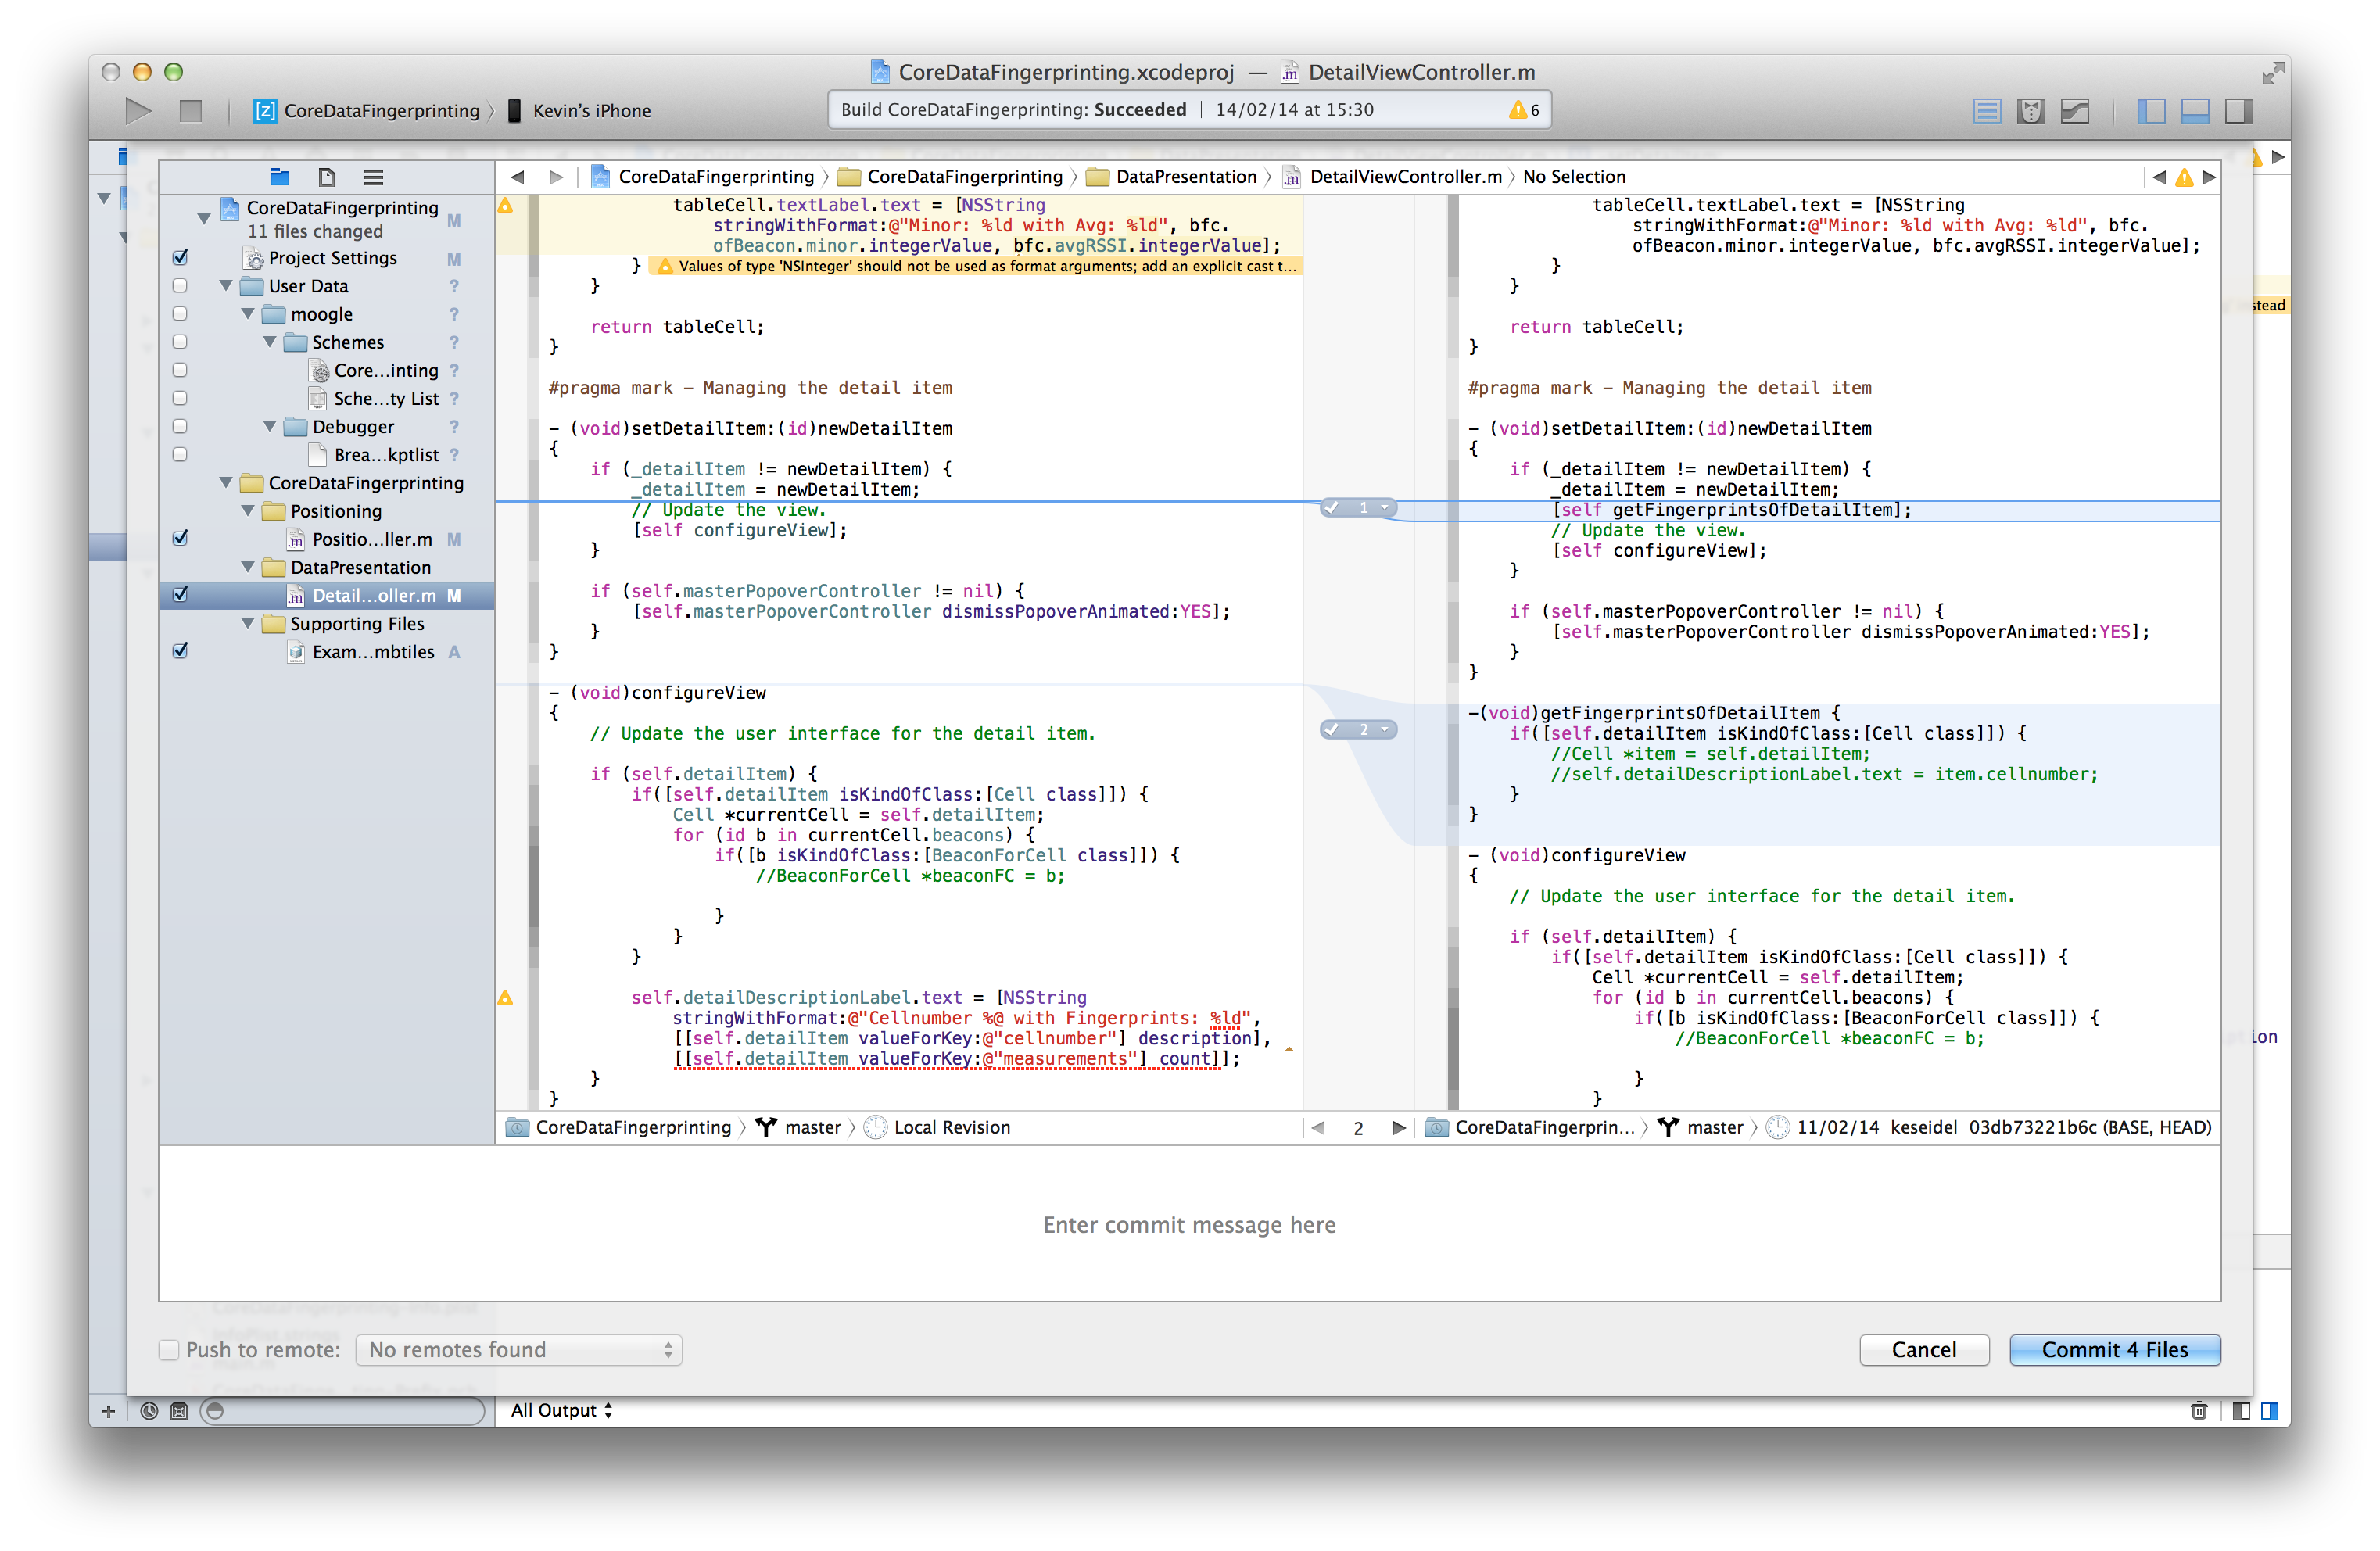
\includegraphics[scale=0.25]{xcode-git-diff}
	\caption{Xcode Versionsverwaltung mit Diff-Anzeige bei einem Commit}
	\label{xcode-git-diff}
\end{figure}



%\chapter{Werkzeuge}
\label{chap:tools}
In diesem Kapitel wird erläutert, welche Hilfsmittel bei der Erstellung des Bachelorarbeit genutzt werden.
Dabei wird näher auf die verwendete Hard- und Software eingegangen und wie sie für die Erstellung und das Testen genutzt wurde.


%%%%%%%%%%%%%%%%%%%%%%%%%%%%%%%%%%%%%%%%%%%%%%%%%%%%%%%%%%%%
\section{Xcode}
\label{sec:tools:xcode}
%%%%%%%%%%%%%%%%%%%%%%%%%%%%%%%%%%%%%%%%%%%%%%%%%%%%%%%%%%%%
Xcode ist eine integrierte Entwicklungsumgebung von Apple, welche es ermöglicht iOS und OS X Applikationen zu programmieren, zu testen und zu debuggen.
Standardmäßig werden dabei die Programmiersprachen \emph{Objective C}, \emph{C} und \emph{C++} unterstützt.

Xcode stellt viele Features für die Programmierung bereit, wie zum Beispiel \emph{code completion}, vorgefertigte \emph{Templates}, einen umfangreichen \emph{Debugger} und eine \emph{iOS-Simulator} für das Testen der Applikationen.

Bei Erstellung einer neuen Applikation kann man unter mehreren Templates wählen, welche jeweils verschiedene Funktionen mit sich bringen. In Abbildung \ref{xcode-templates} lassen sich die verschiedenen Auswahlmöglichkeiten erkennen.

\begin{figure}[htb!]
		\centering
	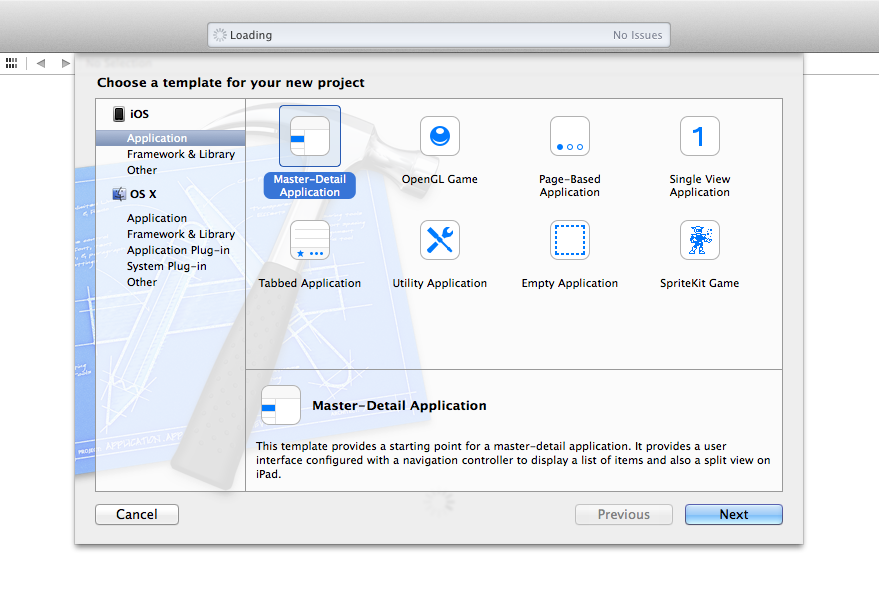
\includegraphics[scale=0.4]{xcode-templates}
	\caption{Auswahlbildschirm der verschiedenen Templates}
	\label{xcode-templates}
\end{figure}

Nach dem man das passende Template gewählt hat, werden die benötigten Dateien angelegt.
Dazu gehören beispielsweise die \emph{AppDelegate} und das \emph{Storyboard}.

Die AppDelegate-Klasse steuert applikationsweite Ereignisse, wie etwa das Aufrufen und Schließen der Applikation. Außerdem wird durch die AppDelegate der aktuelle Zustand der Applikation gespeichert und wiederhergestellt.

Das Storyboard ist eine grafische Oberfläche für die Erstellung des User Interfaces. Es ermöglicht verschiedene Elemente wie zum Beispiel Views, Textfelder, Buttons oder Tabellen einzufügen und diese zu verbinden. Wie in Abbildung \ref{xcode-storyboard} zu erkennen, besteht das Storyboard aus mehreren View Controllern, die jeweils eine gezeigte Szene auf dem Gerät repräsentieren. Die einzelnen View Controller sind mit so gennanten \emph{Segue's} verbunden, welche sich durch bestimmte Aktionen, wie zum Beispiel den Druck auf einen Button, auslösen lassen.

\begin{figure}[htb!]
	\centering
	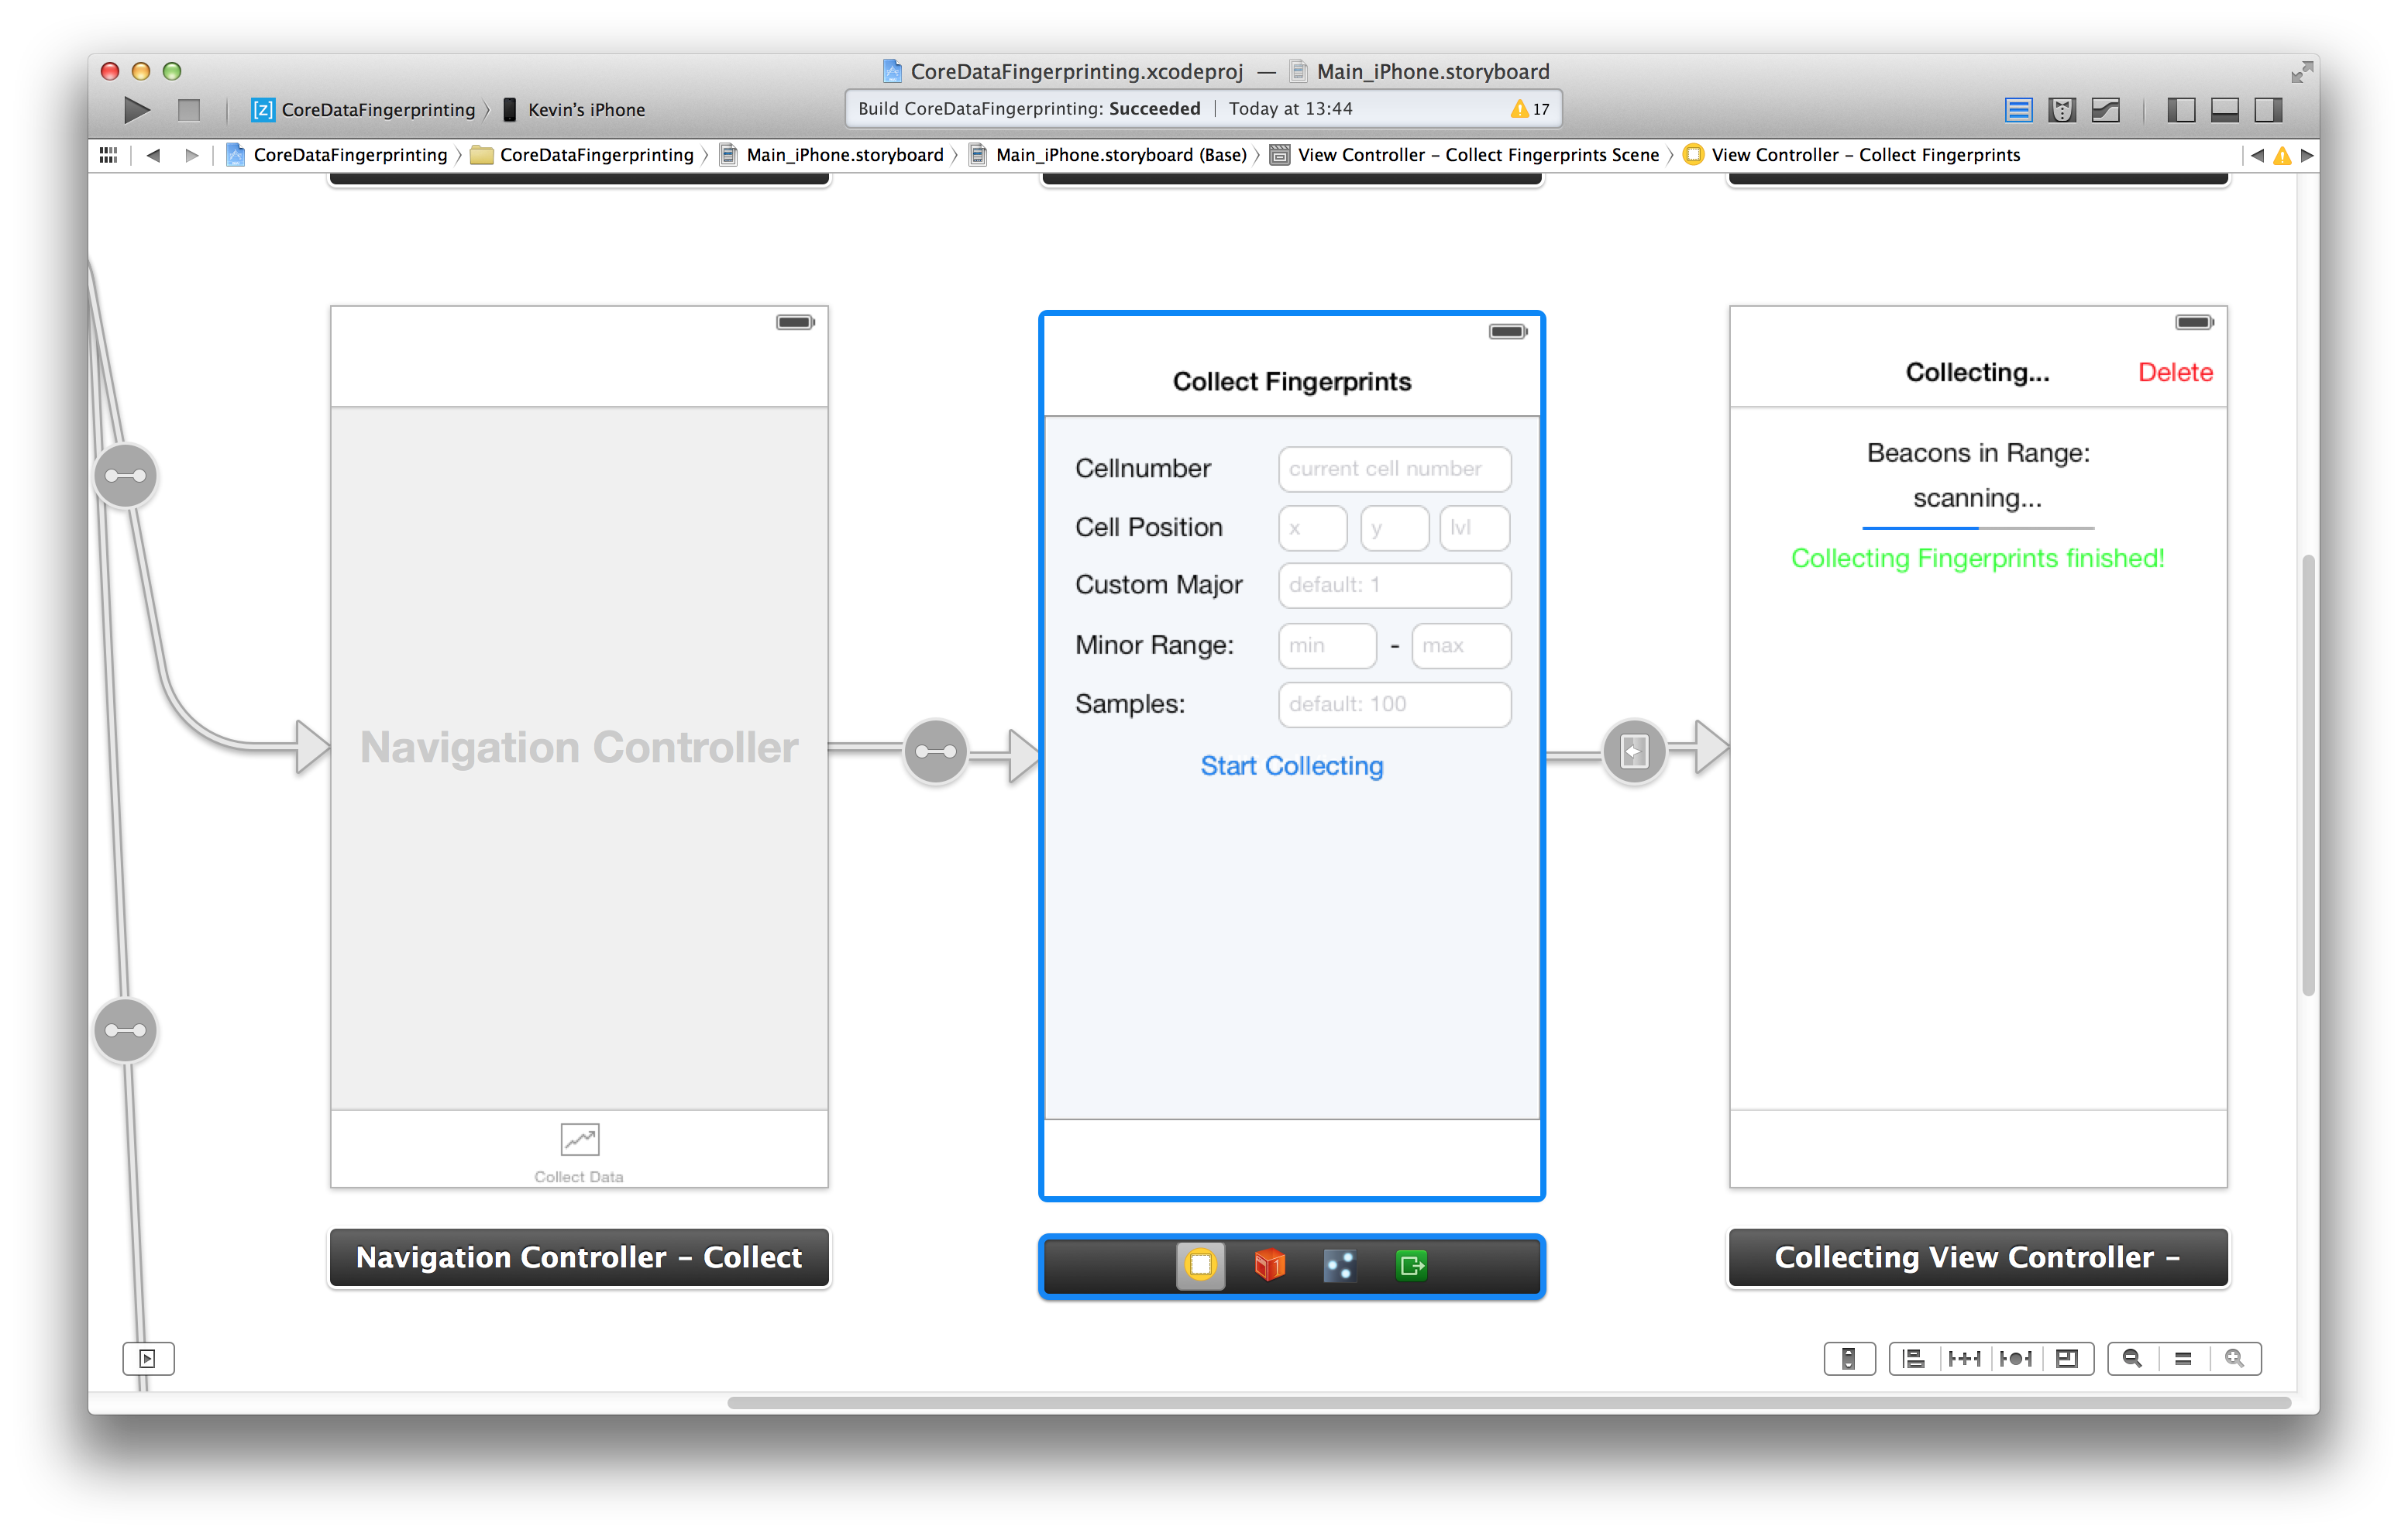
\includegraphics[scale=0.25]{xcode-storyboard}
	\caption{Beispiel eines Storyboards für iPhones}
	\label{xcode-storyboard}
\end{figure}

Das Storyboard bietet außerdem noch die Funktion des \emph{Auto Layout}. Dabei werden sogenannte \emph{Constraints} genutzt, welche die Positionsbeziehungen zwischen den einzelnen Elementen festlegen. Diese Constraints erzeugen so ein dynamisches Interface, welches sowohl im Hochformat, als auch im Querformat ein sauberes und geordnetes Format hat.
In Abbildung \ref{xcode-storyboard-constraints} lassen sich die Abstands und Ausrichtungsbeziehungen zwischen den einzelnen Objekten gut erkennen.

\begin{figure}[htb!]
		\centering
	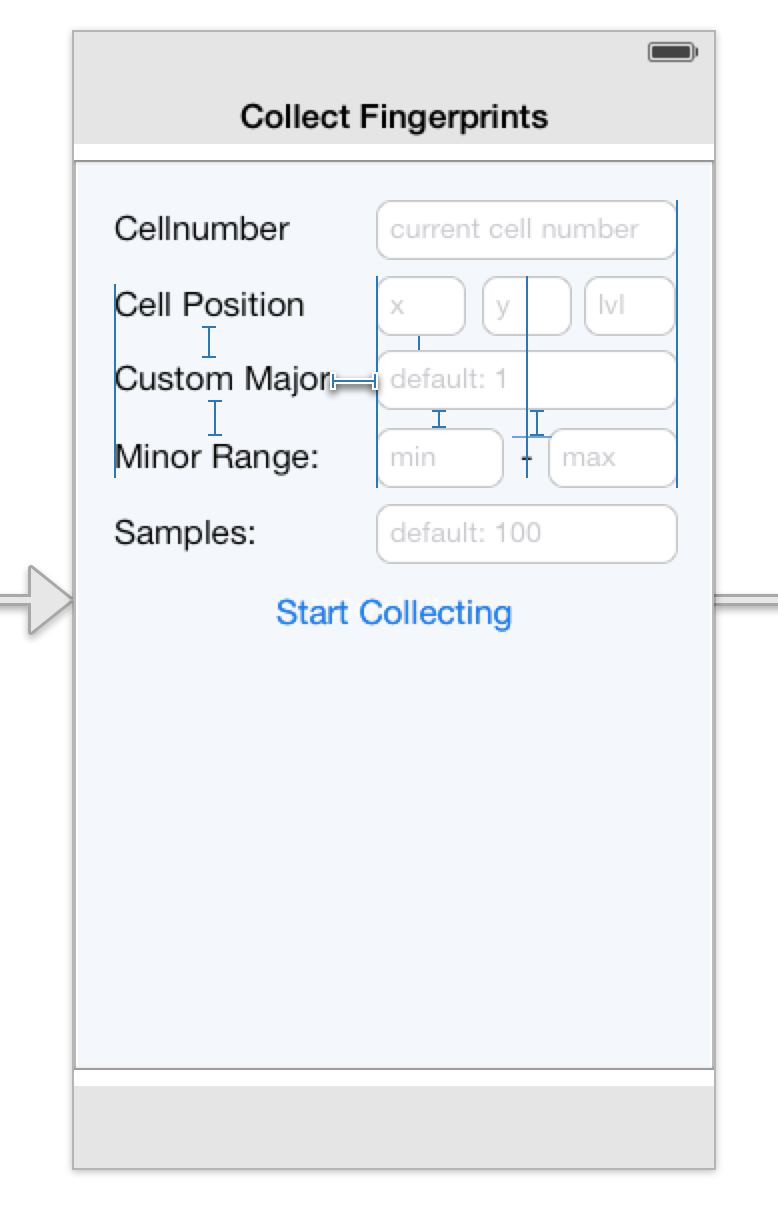
\includegraphics[scale=0.5]{xcode-storyboard-constraints}
	\caption{View Controller mit Constraints}
	\label{xcode-storyboard-constraints}
\end{figure}
\todo{Aufgabe der Constraints beschreiben}

%%%%%%%%%%%%%%%%%%%%%%%%%%%%%%%%%%%%%%%%%%%%%%%%%%%%%%%%%%%%
\section{Objective-C}
\label{sec:tools:objectivec}
%%%%%%%%%%%%%%%%%%%%%%%%%%%%%%%%%%%%%%%%%%%%%%%%%%%%%%%%%%%%
Objective-C ist eine Programmiersprache, welche in den 80er Jahren entwickelt worden ist. Sie ist eine strikte Obermenge von C und erweitert diese um objektorientierte Konzepte. Objective-C ist die Hauptsprache für die Programmierung von Cocoa-Applikationen, wie sie unter iOS und OS X genutzt werden.



%%%%%%%%%%%%%%%%%%%%%%%%%%%%%%%%%%%%%%%%%%%%%%%%%%%%%%%%%%%%
\section{Versionsverwaltung mit Git}
\label{sec:tools:git}
%%%%%%%%%%%%%%%%%%%%%%%%%%%%%%%%%%%%%%%%%%%%%%%%%%%%%%%%%%%%
Xcode bietet für die Versionsverwaltung eine integrierte Git-Unterstützung, welche einfach und schnell zu bedienen ist.
Dabei werden die Differenzen innerhalb des Verzeichnisses bei einem Commit grafisch dargestellt und auch die Unterschiede innerhalb der Datei werden angezeigt.

\begin{figure}[htb!]
		  \centering
	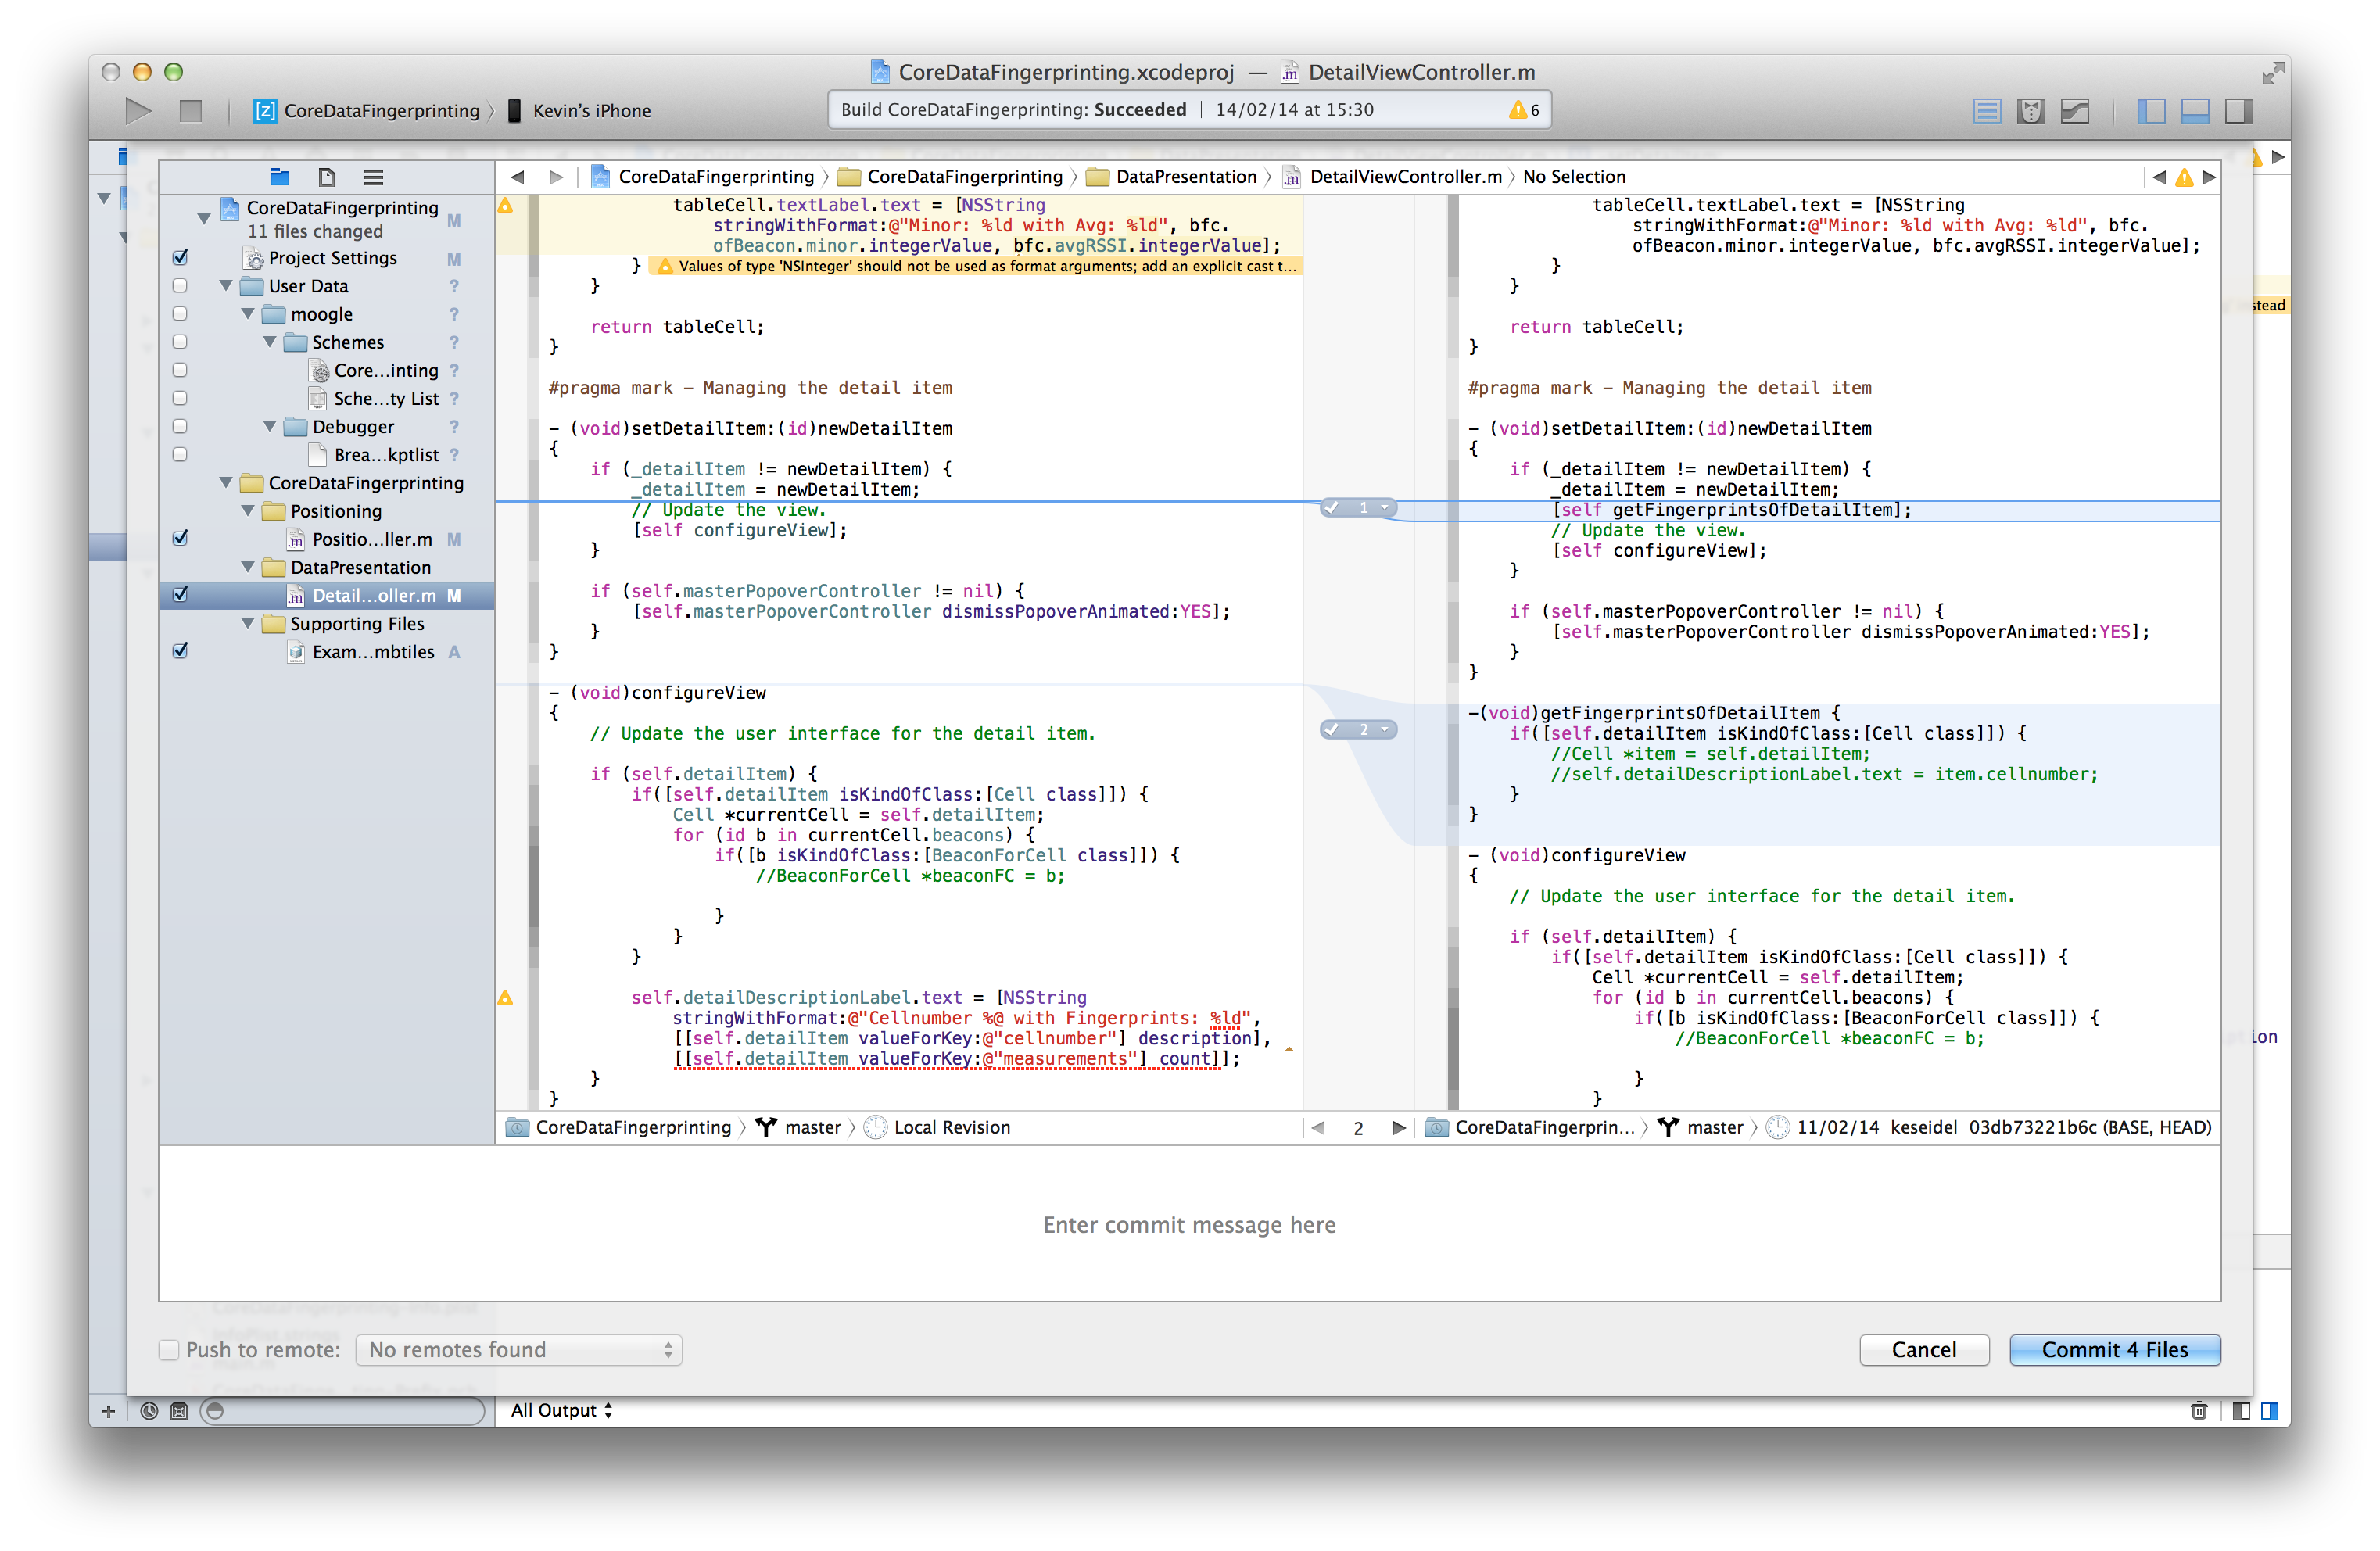
\includegraphics[scale=0.25]{xcode-git-diff}
	\caption{Xcode Versionsverwaltung mit Diff-Anzeige bei einem Commit}
	\label{xcode-git-diff}
\end{figure}

Des Weiteren lassen sich die Änderungen auf Knopfdruck auf einen Server \emph{pushen} und vom Server \emph{pullen}.

Ausserdem lassen sich sehr einfach neue Branches erstellen und ein Mergen der Branches ist auch auf Knopfdruck möglich.


%%%%%%%%%%%%%%%%%%%%%%%%%%%%%%%%%%%%%%%%%%%%%%%%%%%%%%%%%%%%
\section{iOS Developer Program}
\label{sec:iosdevprogram}
%%%%%%%%%%%%%%%%%%%%%%%%%%%%%%%%%%%%%%%%%%%%%%%%%%%%%%%%%%%%
Um eine programmierte Anwendung letztendlich auf einem iOS-Gerät auszuführen, ist die Mitgliedschaft im iOS Developer Program notwendig.
Diese erlaubt das Testen der Anwendung auf dem Gerät, die Veröffentlichung im AppStore und gewährt Zugriff auf das iOS Beta-Programm, um Anwendungen für neue Versionen des Betriebssystems zu optimieren.
Die Mitgliedschaft in diesem \emph{iOS Developer Program} kostet jährlich 99 Dollar. 
Im Rahmen meine Bachelorarbeit wurde mir der Zugang zu diesem Programm von der Universität zur Verfügung gestellt.



%%%%%%%%%%%%%%%%%%%%%%%%%%%%%%%%%%%%%%%%%%%%%%%%%%%%%%%%%%%%
\section{iPhone}
\label{sec:tools:iphone}
%%%%%%%%%%%%%%%%%%%%%%%%%%%%%%%%%%%%%%%%%%%%%%%%%%%%%%%%%%%%
Für die Entwicklung und das Testen der Applikation wurde ein iPhone 5 und ein iPhone 4s verwendet. 
Hauptsächlich wurde das iPhone 5 genutzt, wobei das iPhone 4s eher als Vergleichsgerät diente, um zum Beispiel Messungen zu überprüfen.

Dabei geht es vor allem darum, zu überprüfen in wie weit die Ergebnisse der Messungen übertragbar sind beziehungsweise wie sie sich zwischen den einzelnen Modellen unterscheiden, da diese verschiedene Hardware einsetzen. So setzt das iPhone 4s auf den Broadcom BCM4330-Chipsatz, welches ein Wireless LAN-Chip mit integriertem Bluetooth 4.0 ist. Das iPhone 5 dagegen setzt auf den BCM4334, ebenfalls von Broadcom. 
Aber auch der Aufbau der Antennen und das Material der iPhones unterscheidet sich zwischen diesen beiden Generationen deutlich. 
So ist das iPhone 4s mit einer Glas-Rückseite ausgestattet, wohingegen das iPhone 5 einen Rückseite aus Aluminium besitzt.

Daher ist es wichtig zu vergleichen in wie weit die Änderungen die Empfangsqualität beeinflussen und zu bestimmen, ob eine Übertragung der Ergebnisse möglich ist oder ob jedes Gerät individuell behandelt werden muss.

\begin{figure}[htb!]
		\centering
	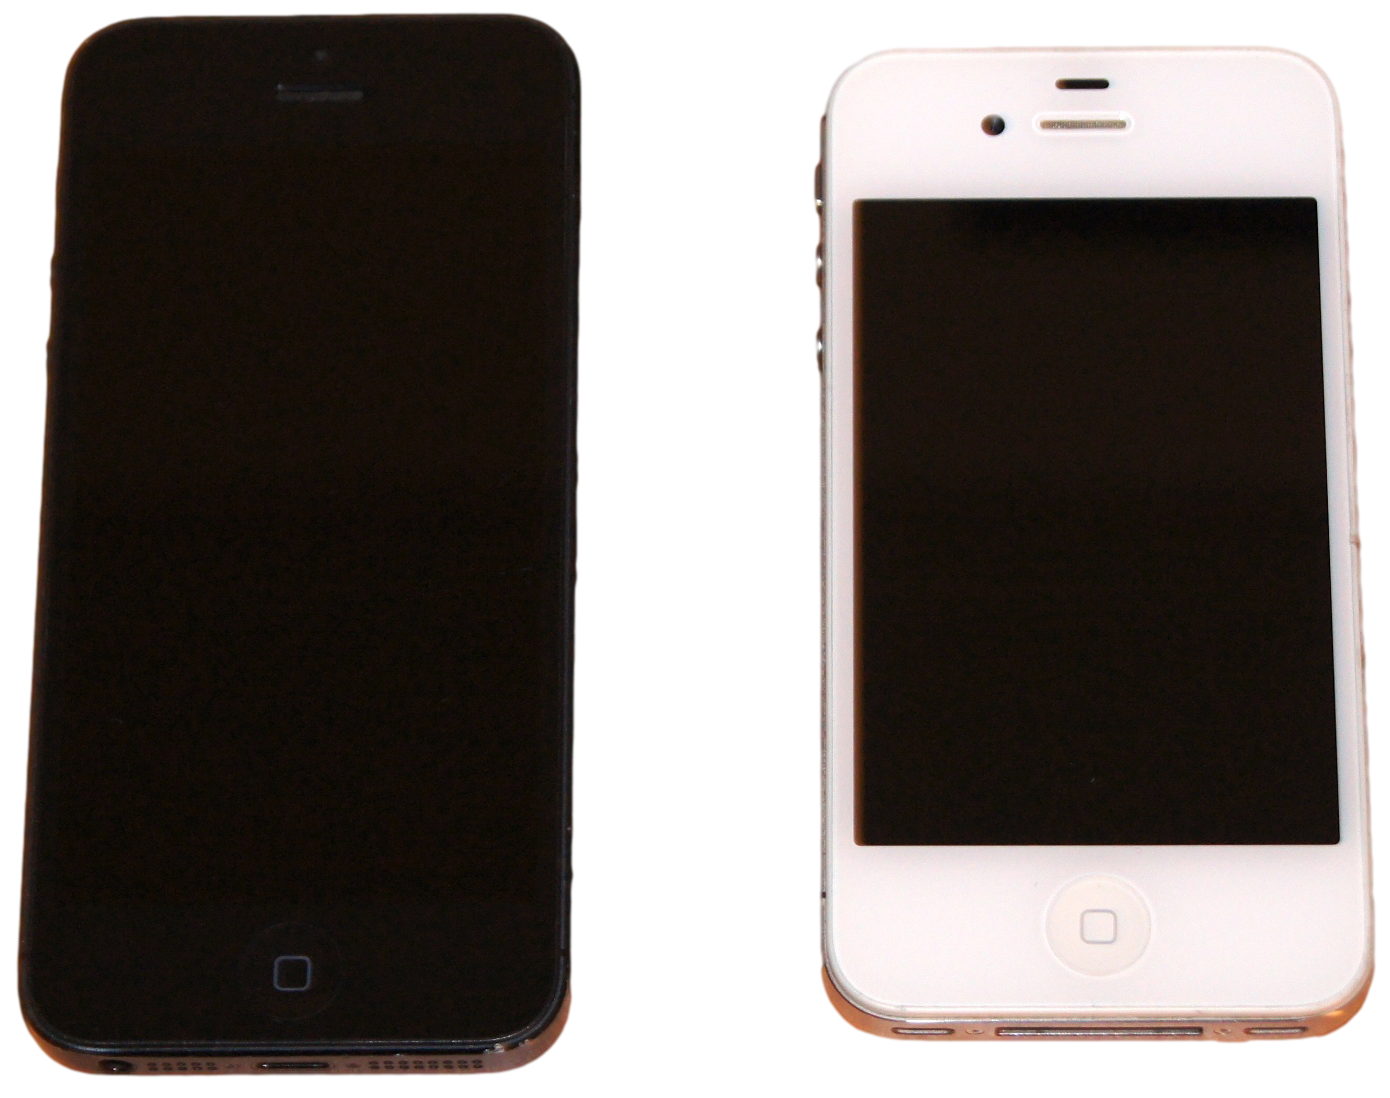
\includegraphics[scale=0.1]{iphones}
	\caption{Die für die Messungen und Tests genutzten iPhones}
	\label{iphones}
\end{figure}




\chapter{Daten und Messungen}
\label{chap:dataandmeasure}

%%%%%%%%%%%%%%%%%%%%%%%%%%%%%%%%%%%%%%%%%%%%%%%%%%%%%%%%%%%%
\section{Mobile iBeacons}
\label{sec:dataandmeasurement:mobilebeacon}
%%%%%%%%%%%%%%%%%%%%%%%%%%%%%%%%%%%%%%%%%%%%%%%%%%%%%%%%%%%%
Die mobilen iBeacon verzichten, wie der Name schon andeutet, auf eine feste Stromquelle und werden ausschließlich mit Batterien betrieben.
Zum Einsatz kommen dabei die sogenannten Knopfzellen, welche mit einer Spannung von 3,0 Volt operieren.
Da Bluetooth Low Energy extrem energiesparend arbeitet, geben die Hersteller der Beacons, die Akkulaufzeit mit bis zu zwei Jahren, ohne einen Batteriewechsel, an. Diese Laufzeit hängt jedoch stark mit der gewählten Signalstärke und dem Sendeintervall zusammen, welche die Laufzeit sehr stark beeinflussen können.

Bisher gibt es nur wenige Hersteller von iBeacons, wobei sich der Großteil der Produkte momentan noch in der Entwicklungsphase befindet. Die genutzten iBeacons von \emph{estimote} und \emph{kontakt.io} sind ebenfalls noch in der Entwicklungsphase und wurden hauptsächlich als Testgeräte für Entwickler ausgegeben. Dabei bleibt jedoch unklar in wie weit sich das fertige Produkt in den technischen Spezifikationen und der Leistung von den aktuellen Prototypen unterscheiden wird.

%%%%%%%%%%%%%%%%%%%%%%%%%%%%%%%%%%%%%%%%%%%%%%%%%%%%%%%%%%%%
\subsection{estimote Beacon}
\label{sec:dataandmeasurement:mobilebeacon:estimote}
%%%%%%%%%%%%%%%%%%%%%%%%%%%%%%%%%%%%%%%%%%%%%%%%%%%%%%%%%%%%
Die Firma \emph{estimote} mit Sitz in Polen, war ein der ersten, die ein funktionstüchtiges iBeacon vorgestellt haben und es in einem \emph{Developer Preview Kit} zum Verkauf anbieten.
Dieses Kit beinhaltet drei verschiedenfarbige Beacons, welche mit einer wiederverwendbaren Klebeschicht an der Unterseite ausgestattet sind. Dies erlaubt ein beliebiges Anbringen und Abziehen der Beacons auf allen glatten Oberflächen.
\begin{figure}[htb!]
		\centering
	\includegraphics[scale=0.1]{estimote-developer-kit}
	\caption{Das Developer-Kit von estimote}
	\label{estimote-developer-kit}
\end{figure}

Im inneren des Beacons befindet sich ein Bluetooth Chipsatz von Nordic Semiconductor, welcher auf einem 32-bit ARM Prozessor beruht und mit einem 2,4Ghz Bluetooth Low Energy Modul arbeitet. Dabei verfügt der über 256 KB Flash-Speicher für Speicherung der Beacon-Konfiguration.
Speziell in den estimote-Beacon wurde dazu noch ein Temperatursensor eingebaut, welcher allerdings momentan noch nicht angesprochen werden kann.

Des Weiteren stellt estimote noch ein SDK für Android und iOS zur Verfügung, welches in Fall des iOS-SDK auf der iBeacons-API basiert, jedoch speziell auf die estimote-Beacons abgestimmt ist. 
Dabei bietet es neben den Funktionen der iBeacon-API noch die Funktionalität, sich mit den estimote Beacons zu verbinden und diese zu programmieren. So erlaubt es zum Beispiel die Signalstärke, das Sendeintervall und die Major-Minor-Informationen zu verändern oder die Firmware der Beacons zu aktualisieren.

Da das SDK, bis auf die Programmierung der Beacons, keine Vorteile gegenüber dem Core Location-Framework mit der iBeacons-API bietet, wurde jedoch auf die Verwendung verzichtet.

%%%%%%%%%%%%%%%%%%%%%%%%%%%%%%%%%%%%%%%%%%%%%%%%%%%%%%%%%%%%
\subsection{kontakt.io Beacon}
\label{sec:dataandmeasurement:mobilebeacon:kontaktio}
%%%%%%%%%%%%%%%%%%%%%%%%%%%%%%%%%%%%%%%%%%%%%%%%%%%%%%%%%%%%
Ein weiteres Unternehmen, welches sich eine eigene iBeacons-Lösung anbietet ist \emph{kontakt.io}. Auch hier ist noch kein finales Produkt erhältlich, sondern nur ein \emph{Development Kit}, welches zehn Beacons enthält. 
Die Beacons sind relativ schlicht gehalten und das Innere ist sehr einfach zugänglich, sodass ein Batteriewechsel ohne Umstände möglich ist.


\begin{figure}[htb!]
		\centering
	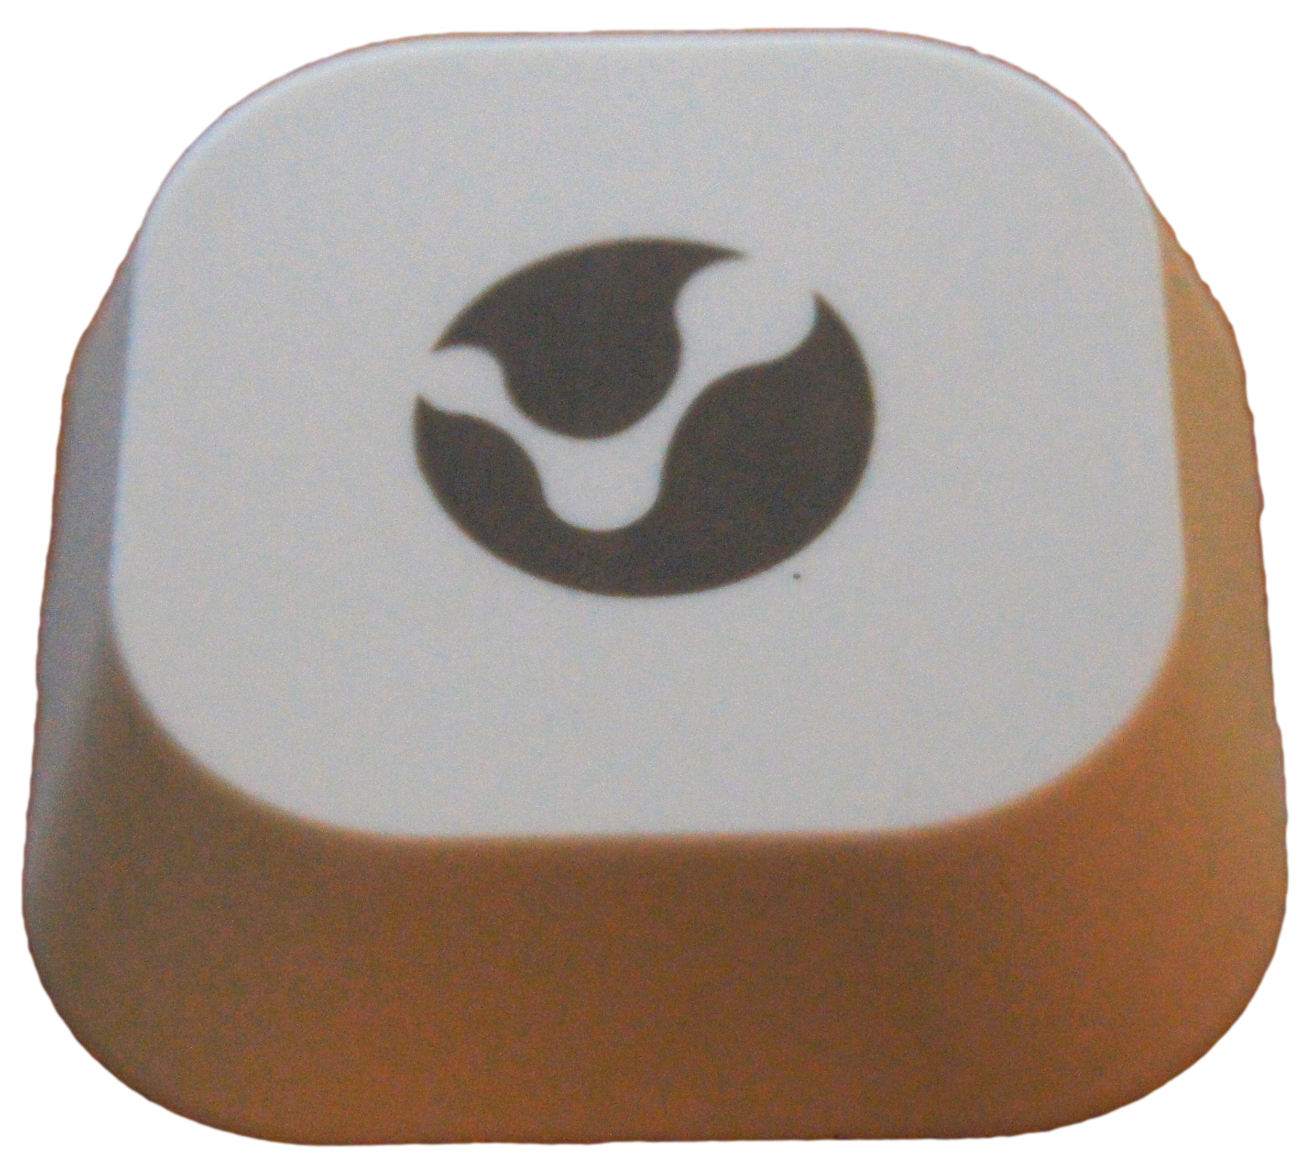
\includegraphics[scale=0.1]{kontakt-beacon-outside}
	\caption{Kontakt.io Beacon}
	\label{kontakt-beacon-outside}
\end{figure}

Die Beacons von \emph{kontakt.io} basieren dabei auf dem BLE113 Chipsatz von \emph{bluegiga}, welcher über 256 KB Flash-Speicher verfügt und einen 8051 Mikrocontroller von Intel nutzt.


Auch kontakt.io bietet ein eigenes SDK an, welches im Gegensatz zu dem SDK von \emph{estimote} nicht nativ für die einzelnen Plattformen entworfen wurde, sondern online über eine REST-Schnittstelle arbeitet.
Dabei stellt \emph{kontakt.io} ein Webpanel zur Verfügung, in welchem man die einzelnen Beacons mit ihrem UUID, Major und Minor-Wert registriert und jedem den jeweiligen Ort beziehungsweise die Funktion zuweisen kann. 
Auch auf die Verwendung dieses SDK wurde verzichtet.


%%%%%%%%%%%%%%%%%%%%%%%%%%%%%%%%%%%%%%%%%%%%%%%%%%%%%%%%%%%%
\section{Stationäre iBeacons}
\label{sec:dataandmeasurement:stationarybeacon}
%%%%%%%%%%%%%%%%%%%%%%%%%%%%%%%%%%%%%%%%%%%%%%%%%%%%%%%%%%%%
Neben den mobilen iBeacons, welche mittels Batterien betrieben werden, gibt es auch stationäre iBeacons, welche auf eine stetige Anbindung an das Stromnetz angewiesen sind.
Dabei gibt es verschiedene Ansätze.
Zum Einen bieten zum Beispiel \emph{PayPal} und \emph{Radius Networks} einen Ansatz, bei dem die komplette Technik in einen USB-Stick integriert wird und über ein USB-Netzteil an jeder Steckdose betrieben werden kann. Die verwendete Technik dieser Beacons entspricht denen der batteriebetriebenen Beacons.

Eine andere Lösung ist die Nutzung eines Bluetooth 4.0-kompatiblen USB-Dongles an einem Computer. Dieser kann mit entsprechender Software zu einem iBeacon umfunktioniert werden.

%%%%%%%%%%%%%%%%%%%%%%%%%%%%%%%%%%%%%%%%%%%%%%%%%%%%%%%%%%%%
\subsection{Raspberry Pi als iBeacon}
\label{sec:dataandmeasurement:stationarybeacon:raspberrypi}
%%%%%%%%%%%%%%%%%%%%%%%%%%%%%%%%%%%%%%%%%%%%%%%%%%%%%%%%%%%%
Der Raspberry Pi ist ein Mini-Computer, welcher auf einem ARM-Prozessor basiert und als günstiger Computer für Programmiereinsteiger konzipiert wurde. Der kleine Computer ermöglicht aber auch andere Einsatzgebiete, zum Beispiel als Beacon.

Um den Raspberry Pi zu einem Beacon umzufunktionieren wurde eine Linux-Distribution auf dem Gerät installiert und ein Bluetooth-Dongle über USB angeschlossen. Dabei kam ein Modul von \emph{Plugable Technologies} zum Einsatz, welches spezielle Bluetooth 4.0 und Linux-Unterstützung bietet.
Für die Umfunktionierung zum iBeacon wurde die Bluetooth-Implementierung \emph{blueZ} eingesetzt, welche es erlaubt das Bluetooth-Modul anzusprechen und spezifische Nachrichten über Bluetooth zu versenden.
Diese Möglichkeit den Raspberry Pi als iBeacon zu nutzen, wurde von der Firma Radius Network vorgestellt. Diese bieten ein ausführliches Tutorial für die Nutzung des Raspberry Pi als iBeacon auf ihrer Webseite an (\citet{radiusraspberry}), welches von mir genutzt wurde, um den Raspberry Pi zu konfigurieren.

%%%%%%%%%%%%%%%%%%%%%%%%%%%%%%%%%%%%%%%%%%%%%%%%%%%%%%%%%%%%
\section{Physikalische Grundlagen}
\label{sec:dataandmeasurement:physics}
%%%%%%%%%%%%%%%%%%%%%%%%%%%%%%%%%%%%%%%%%%%%%%%%%%%%%%%%%%%%
Im Vergleich zu Kabelverbindungen, wo die Ausbreitung des Signals entlang eines bestimmten Leiters geschieht, ist die Ausbreitung eines drahtlosen Signals von deutlich mehr Faktoren abhängig.

\textbf{Dämpfung}

Dämpfung ist die Schwächung der Energie, mit welcher das Signal übertragen wird. Diese tritt auch bei einer freien Sichtverbindung zwischen Sender und Empfänger auf. Die Verringerung der Leistung ist dabei abhängig von der Ausgangssendeleistung $P_0$ und der Entfernung $r$ zwischen Sender und Empfänger. Die letztlich am Empfänger ankommende Signalstärke $P_r$ berechnet sich dabei wie folgt:

\begin{equation}
	P_r = \frac{P_0}{r^{2}} 
\end{equation}

Die Abschwächung des Signals resultiert aus der Art der Aussendung. Da die hier verwendeten Beacons einem Punktstrahler entsprechen, wird die anliegende Signalstärke auf eine Kugeloberfläche verteilt. Die Kugeloberfläche $O$ lässt sich dabei abhängig vom Radius $r$ mittels der Formel $O = 4 \pi r^{2}$ berechnen. Die Oberfläche vergrößert sich damit quadratisch zum Radius.

\textbf{Abschattung}

Die Abschattung ist eine stärkere Form der Dämpfung, welche durch Objekte zwischen der Signalquelle und dem Empfänger verursacht wird. Die Abschattung ist dabei abhängig von der Frequenz des Signals und der Geschaffenheit des Objektes. Bei höherer Frequenz ist eine stärkere Abschattung des Signals gegeben.

\textbf{Reflexion}

An größeren Oberflächen kann es zu Reflexionen des Signals kommen. Dabei trifft es auf die Oberfläche und wird dann in abgeschwächter Form reflektiert.

\textbf{Streuung}

Ähnlich der Reflexion trifft das Signal auf eine Oberfläche, wird dabei jedoch aufgespalten und in verschiedene Richtung abgelenkt.

\textbf{Mehrwegeausbreitung}

Durch die obene genannten Effekte ist es möglich, das ein Signal einen Empfänger auf mehreren Wegen erreicht. Dabei ist die Signalstärke stark abhängig von dem zurückgelegtem Weg. Ausserdem unterscheiden sich die Laufzeiten der Signale, da diese ebenfalls vom Weg abhängig sind. Dadurch kann es auch zu Überlagerungen zwischen Signalen kommen, welche zur gleichen Zeit gesendet wurden, jedoch zu unterschiedelichen Zeiten beim Empfänger eintreffen. 
Durch diese Phasenverschiebung kann das Signal zusätzlich abgeschwächt werden.


%%%%%%%%%%%%%%%%%%%%%%%%%%%%%%%%%%%%%%%%%%%%%%%%%%%%%%%%%%%%
\section{Außenmessungen}
\label{sec:dataandmeasurement:outdoormeasure}
%%%%%%%%%%%%%%%%%%%%%%%%%%%%%%%%%%%%%%%%%%%%%%%%%%%%%%%%%%%%

%%%%%%%%%%%%%%%%%%%%%%%%%%%%%%%%%%%%%%%%%%%%%%%%%%%%%%%%%%%%
\section{Innenraummessungen}
\label{sec:dataandmeasurement:indoormeasure}
%%%%%%%%%%%%%%%%%%%%%%%%%%%%%%%%%%%%%%%%%%%%%%%%%%%%%%%%%%%%
Um die Leistungsfähigkeit und das Verhalten der Beacons in Innenräume zu testen und darzustellen, wurden verschiedene Messungen durchgeführt. Dazu wurden zum einen die mobilen Beacons verwendet und zum Anderen der Raspberry Pi, als stationäres Beacon.
Die Messungen wurden dabei sowohl mit dem iPhone 5 als auch mit dem iPhone 4s durchführt, um auch hier die Unterschiede zwischen den einzelnen Modellen zu erfassen.


Zuerst wurden die Messungen mit den mobilen Beacons, hier die \emph{kontakt.io}-Beacons, durchgeführt.
Diese wurden in einem leeren, nur an den Wänden bestellten, Raum durchgeführt, wobei immer freie Sicht zwischen den Beacons und den Empfangsgeräten bestand. Für jede Entfernung wurden dabei 100 Stichproben genommen, jeweils eine pro Sekunde.
%%%%%%%%%%%%%%%%%%%%%%%%%%%%%%%%%%%%%%%%%%%%%%%%%%%%%%%%%%%%
% figure of signal strnegth
%%%%%%%%%%%%%%%%%%%%%%%%%%%%%%%%%%%%%%%%%%%%%%%%%%%%%%%%%%%%
\begin{figure}[h!]
	\centering
	\begin{minipage}[t]{5cm}
		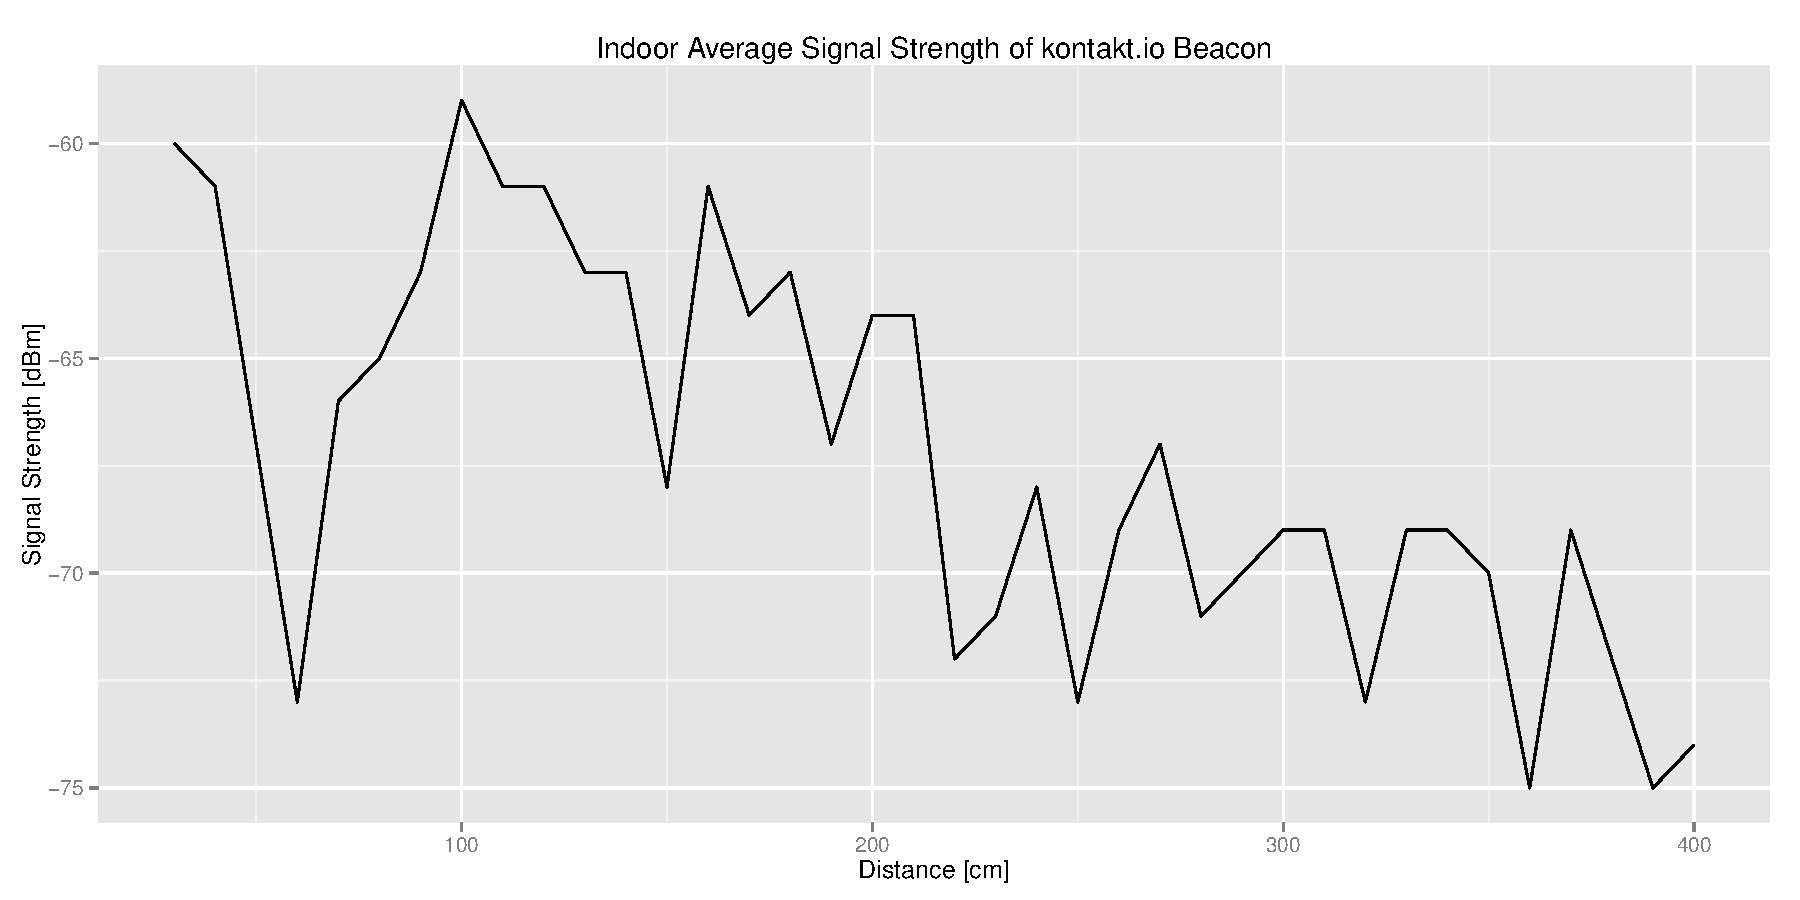
\includegraphics[scale=0.2]{avgiphone5}
		\caption{Messung des iPhone 5}
		\label{avgiphone5-signalstrength}
	\end{minipage}
	\hspace{2cm}
	\begin{minipage}[t]{5cm}
			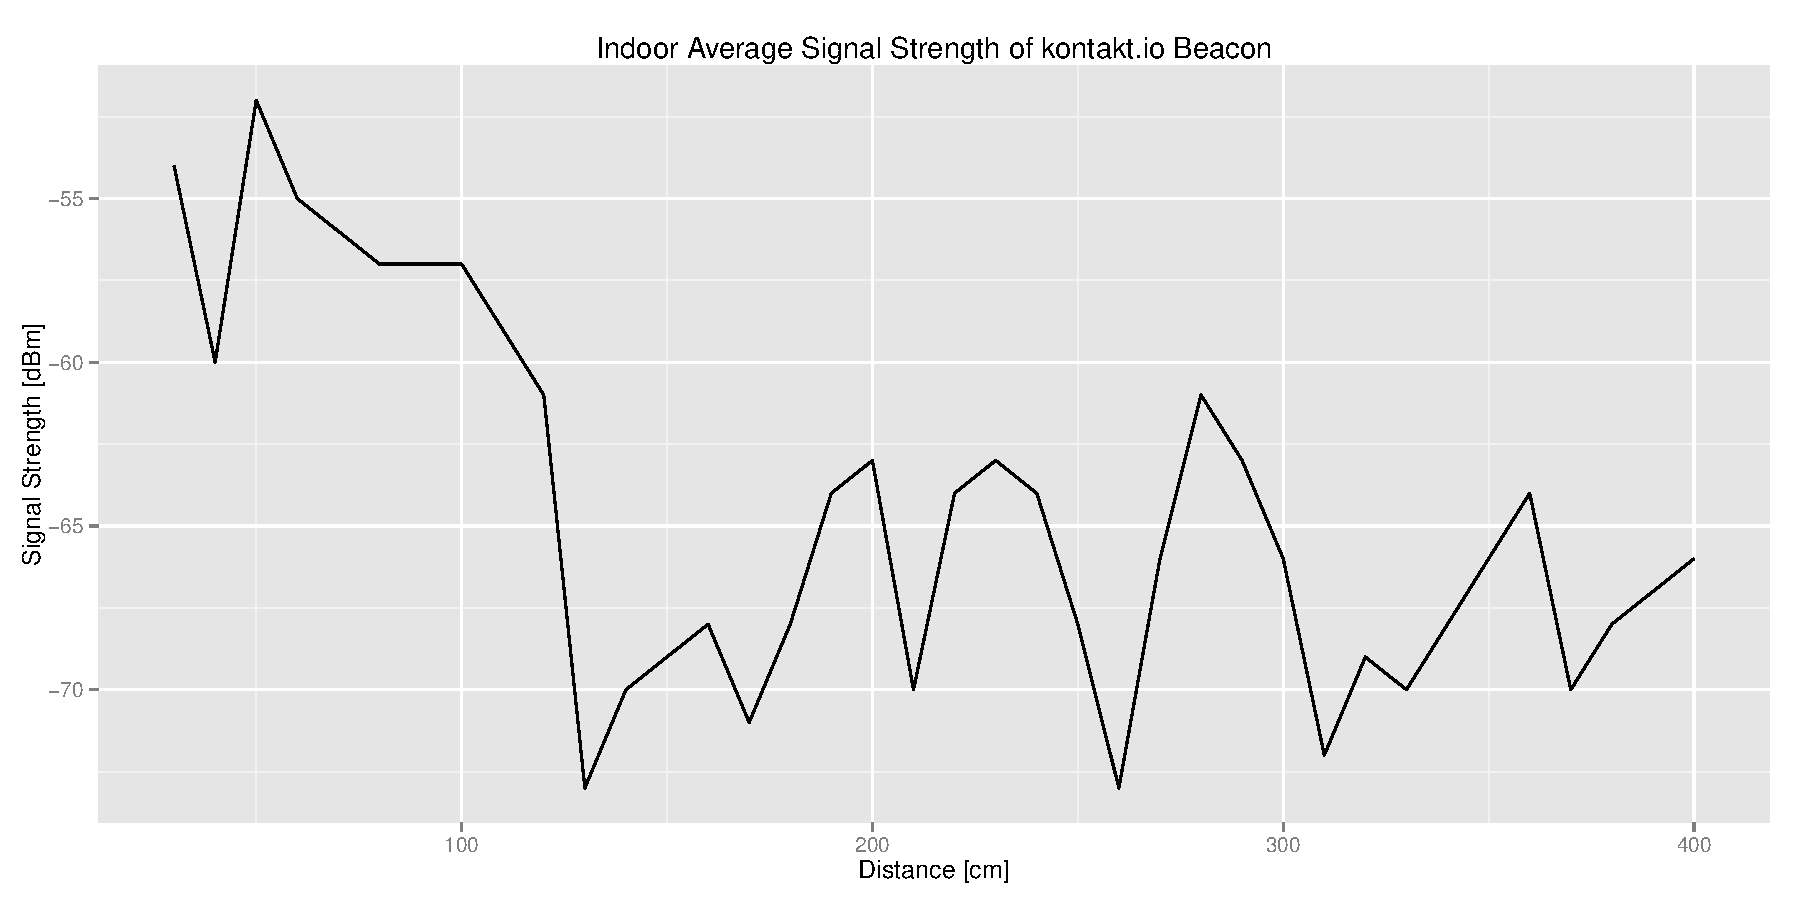
\includegraphics[scale=0.2]{avgiphone4s}
			\caption{Messung des iPhone 4s}
			\label{avgiphone4s-signalstrength}
	\end{minipage}
		\caption{Durchschnittliche Signalstärke eines kontakt.io Beacons}
		\label{signalstrength}
\end{figure}

In Abbildung \ref{avgiphone5-signalstrength} und Abbildung \ref{avgiphone4s-signalstrength} lässt sich dabei sehr gut erkennen, das die Signalstärke, nicht wie eigentlich erwartet stetig abnimmt, sondern relativ stark schwankt. Dies ist darauf zurückzuführen, dass in Innenräumen sowohl Wände, als auch Gegenstände im Raum, das Bluetooth-Signal reflektieren oder blockieren und so die Ergebnisse verfälschen.
Des Weiteren ist zu erkennen, dass die Ergebnisse zwischen den verschiedenen iPhone-Modellen deutlich voneinander abweichen. Das lässt darauf schließen, das der verbaute Chipsatz beziehungsweise die verbaute Antenne innerhalb der Gerät die Ergebnisse deutlich beeinflusst und die Werte daher nur schwer übertragbar sind.

Ein weiterer wichtiger Punkt ist die Untersuchung der Stabilität des Signal. Dabei wurden die gleichen Daten wie zuvor verwendet, jedoch um die minimalen und maximalen Werte ergänzt. In Abbildung \ref{all-iphone5} lässt sich dabei gut erkennen, das die Ergebnisse eine ähnliche Tendenz haben, aber sich dennoch über einen sehr großen Bereich der Signalstärke verteilen.

\begin{figure}[htb!]
		\centering
	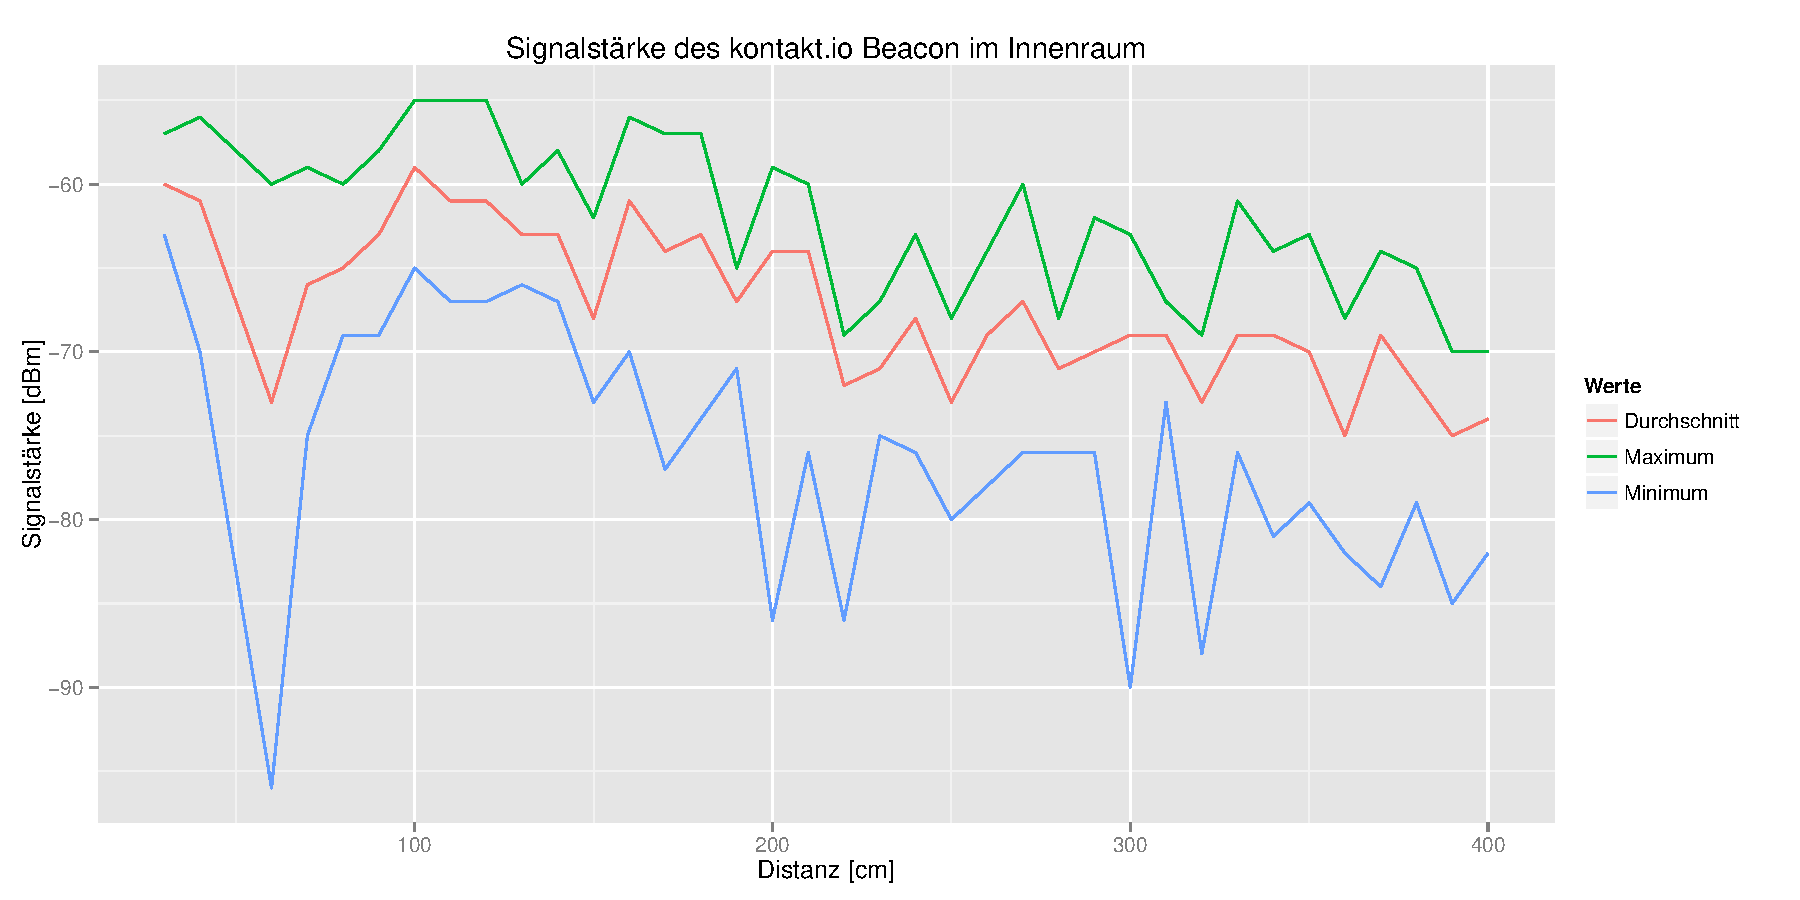
\includegraphics[scale=0.5]{alliphone5}
	\caption{Minimale, maximale und durchschnittliche Signalstärke des Beacons gemessen vom iPhone 5}
	\label{all-iphone5}
\end{figure}


Zusätzlich wurde untersucht in wie weit sich die Sendeleistung und Signalqualität der batteriebetriebenen Beacon von stationären Beacons unterscheidet.
Dazu wurde der gleiche Messaufbau wie zuvor genutzt, jedoch das \emph{kontakt.io} Beacon durch den Raspberry Pi ausgetauscht. Danach wurden die gleichen Messungen erneut durchgeführt.

\begin{figure}[htb!]
		\centering
	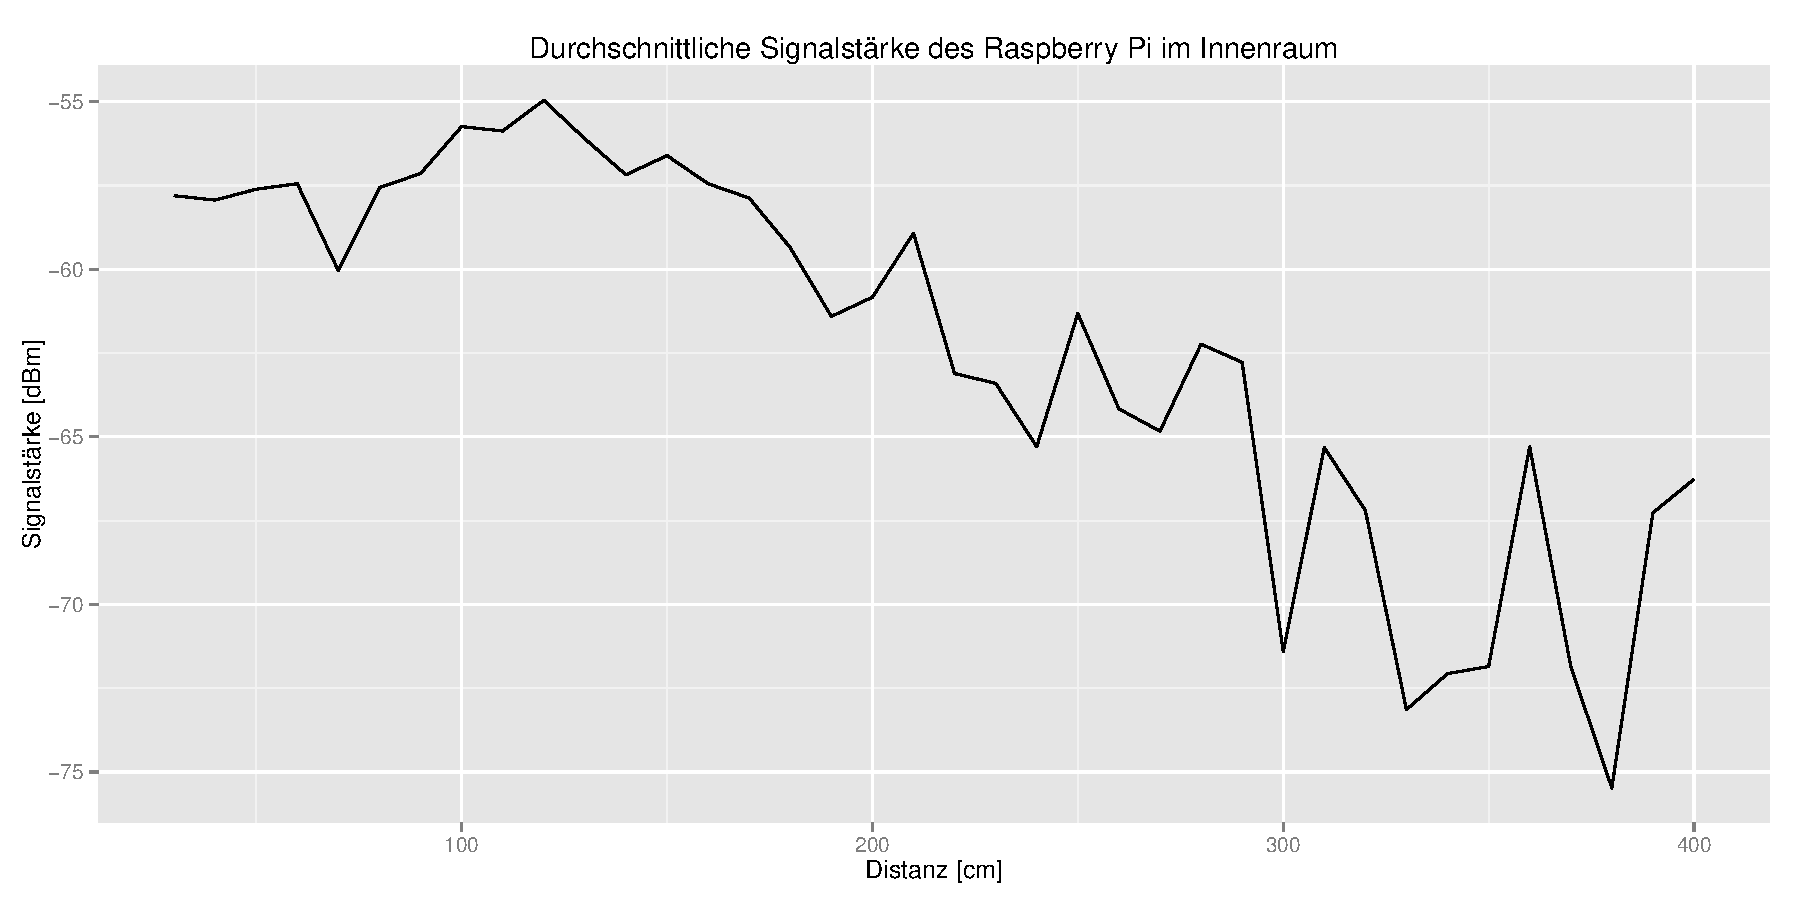
\includegraphics[scale=0.5]{avgiphone5_raspberry}
	\caption{Durchschnittliche Signalsteäines Raspberry Pi Beacons}
		\label{avgiphone5_raspberry}
\end{figure}

Wie aus Abbildung \ref{avgiphone5_raspberry} zu entnehmen, sind die Ergebnisse im Vergleich zu der Messung der kontakt.io Beacons näher am erwarteten Ergebnis, welches eine konstante Abnahme der Signalstärke sein sollte. Es sind jedoch immernoch einige Ausreißer zu erkennen. Bei der Betrachtung der minimalen und maximalen Signalstärken fällt auch auf, dass die ähnlich stark schwanken, wie schon zuvor bei den kontakt.io Beacons. Die Stabilität des Signal des stationären Beacons ist also genauso schwach beziehungsweise noch schwächer als die des batteriebetriebenen Beacons. Dies wird in Abbildung \ref{alliphone5_raspberry} nocheinmal deutlich.

\begin{figure}[htb!]
		\centering
	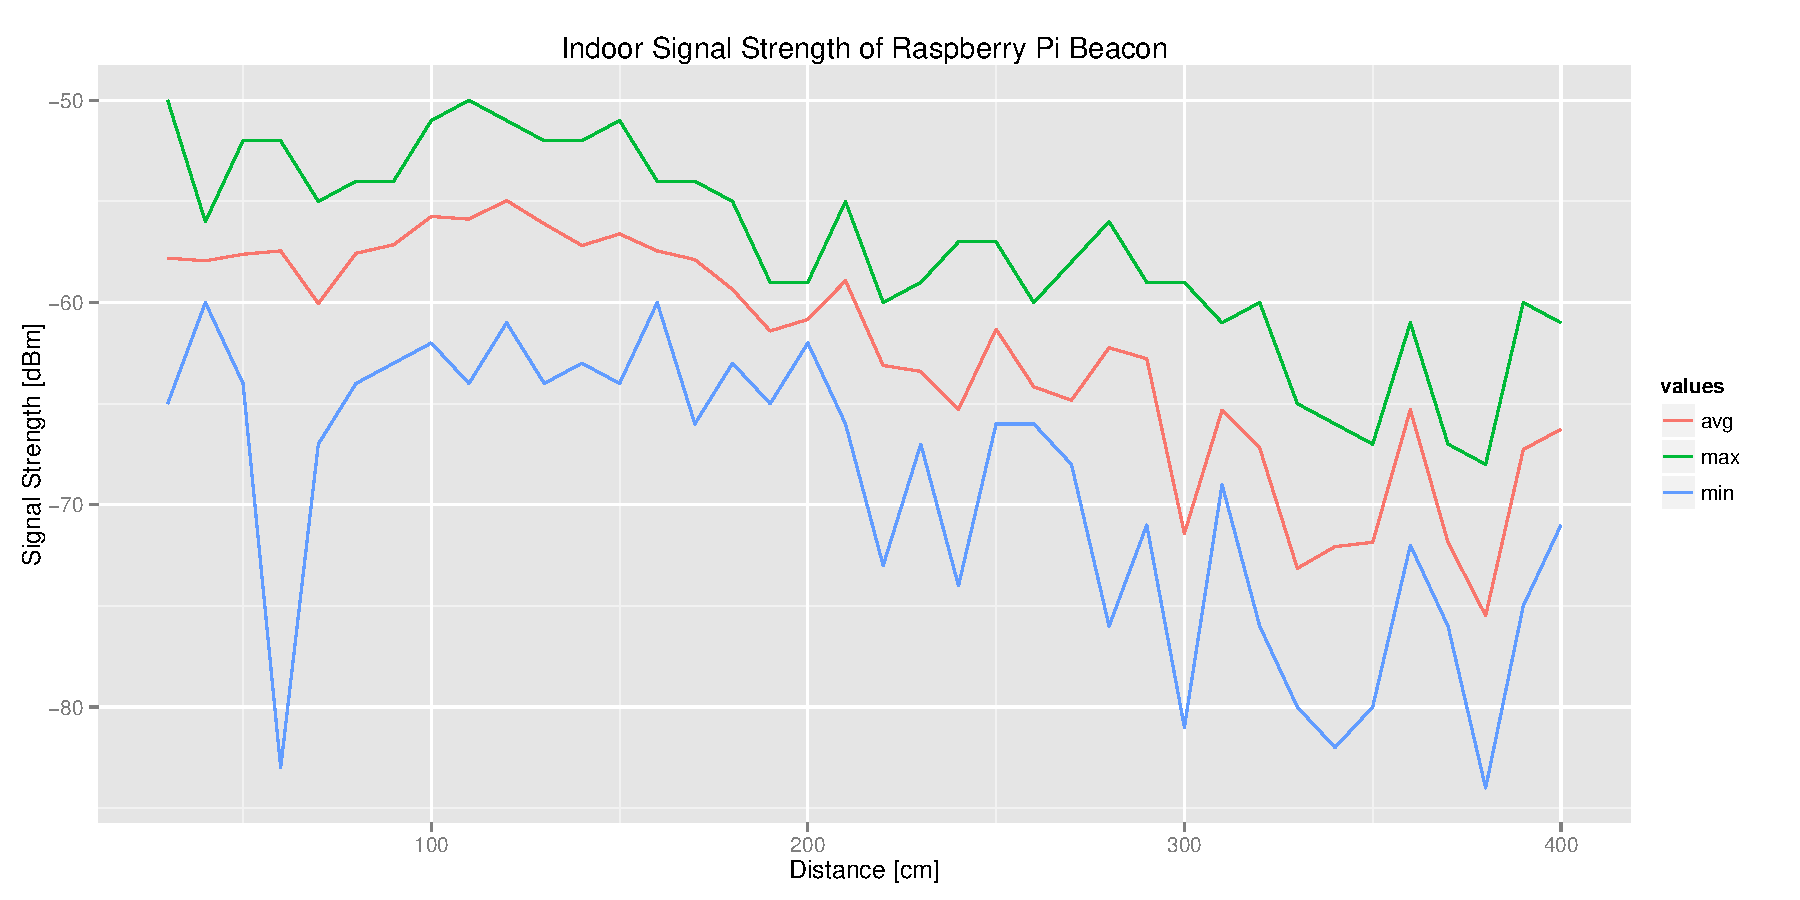
\includegraphics[scale=0.5]{alliphone5_raspberry}
	\caption{Minimale, maximale und durchschnittliche Signalstrke des Raspberry Pi gemessen vom iPhone 5}
	\label{alliphone5_raspberry}
\end{figure}

Für die weiteren Test und Messungen wurden daher die \emph{kontakt.io} Beacons verwendet, da die beiden zur Verfügung stehenden Beacons sich in Signalstärke und Stabilität nicht zu stark unterscheiden, von den \emph{kontakt.io} Beacons jedoch deutlich mehr Exemplare verfügbar sind und diese deutlich variabler im Bezug auf die Positionierung der Beacons sind.


%%%%%%%%%%%%%%%%%%%%%%%%%%%%%%%%%%%%%%%%%%%%%%%%%%%%%%%%%%%%
\section{Mögliche Störfaktoren}
\label{sec:dataandmeasurement:interferencefactor}
%%%%%%%%%%%%%%%%%%%%%%%%%%%%%%%%%%%%%%%%%%%%%%%%%%%%%%%%%%%%
Wie die obigen Messungen zeigen, weichen die realen Ergebnisse stark von den, durch die physikalischen Ausbreitungseigenschaften der elektromagnetischen Wellen, angenommenen Ergebnissen ab. Dies hängt vorallem damit zusammen, dass die Antenne der Beacons nicht gerichtet ist, sondern in alle Richtungen sendet. Dies führt dazu, dass das Signal der Beacons von diversen Flächen im Raum reflektiert und so nicht auf direktem Weg zum Endgerät gelangt. 

Ein weiterer wichtiger Störfaktor ist der Benutzer selbst, da der menschliche Körper größtenteils aus Wasser besteht, welche elektromagnetische Wellen abschirmt. Daher ist zu beobachten, dass die Ausrichtung des Nutzers einen deutlichen Einfluss auf die Signalstärke nimmt. In Abbildung \ref{boxplotiPhone5Body} ist diese Auswirkung des Körpers deutlich zu erkennen. Hierbei wurden jeweils aus zwei Metern Entfernung 100 Stichproben der Signalstärke genommen. Einmal mit freier Sicht zum Beacon und einmal mit dem Körper zwischen Beacon und iPhone. 

\begin{figure}[htb!]
		\centering
	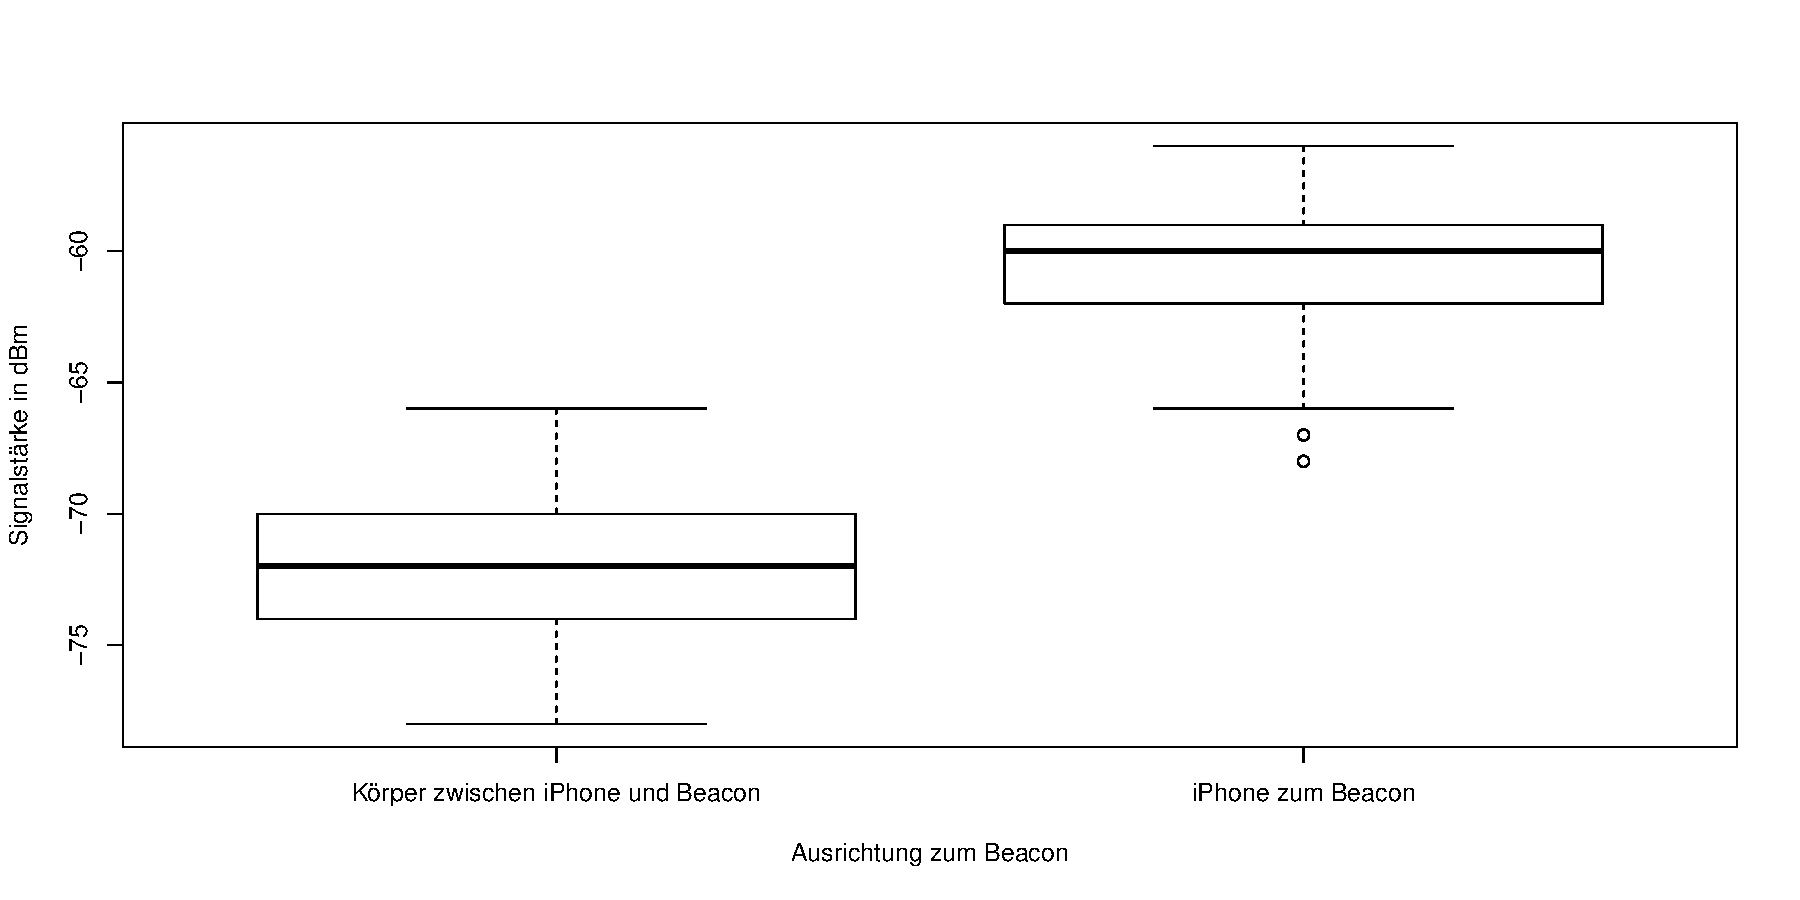
\includegraphics[scale=0.5]{boxplotiPhone5Body}
	\caption{Signalstärke bei 2m Entfernung zum Beacon}
	\label{boxplotiPhone5Body}
\end{figure}

Auf der Abbildung ist deutlich zu erkennen wie der Körper die Signalstärke verringert. Dieser Faktor muss also in die Positionsbestimmung einbezogen werden.

Zusätzlich zum Körper kann es an realen Einsatzorten weitere Gegenstände geben, welche das Signal abschirmen beziehungsweise abschwächen, wie zum Beispiel Wände oder Möbelstücke.
\chapter{Umsetzung und Implementation}
\label{chap:implementation}


%%%%%%%%%%%%%%%%%%%%%%%%%%%%%%%%%%%%%%%%%%%%%%%%%%%%%%%%%%%%
\section{Initialisierung und Beacon-Daten}
\label{sec:implementation:initandbeacon}
%%%%%%%%%%%%%%%%%%%%%%%%%%%%%%%%%%%%%%%%%%%%%%%%%%%%%%%%%%%%

%%%%%%%%%%%%%%%%%%%%%%%%%%%%%%%%%%%%%%%%%%%%%%%%%%%%%%%%%%%%
% Generating the project and setup the storyboard
%%%%%%%%%%%%%%%%%%%%%%%%%%%%%%%%%%%%%%%%%%%%%%%%%%%%%%%%%%%%

Für die Implementierung unter iOS müssen zunächst einige grundlegende Programmbestandteile erzeugt und eingerichtet werden.
Wie bereits in Kaptiel \ref{sec:tools:xcode} gezeigt, gibt es bei der Erstellung eines neuen Projektes in Xcode verschiedene Vorlage, aus welchen gewählt werden kann. Für diese Applikation wurde die Vorlage der \emph{Master-Detail Application} gewählt, da diese eine CoreData-Unterstützung mit sich bringt. Ausserdem lassen sich über die Master-Detail Applikation die bereits gemessenen Werte in einer Tabellen anzeigen und zusätzlich, bei Klick auf die Tabellenzelle, weitere Informationen zu der Daten ausgeben.

\begin{figure}[htb!]
		\centering
	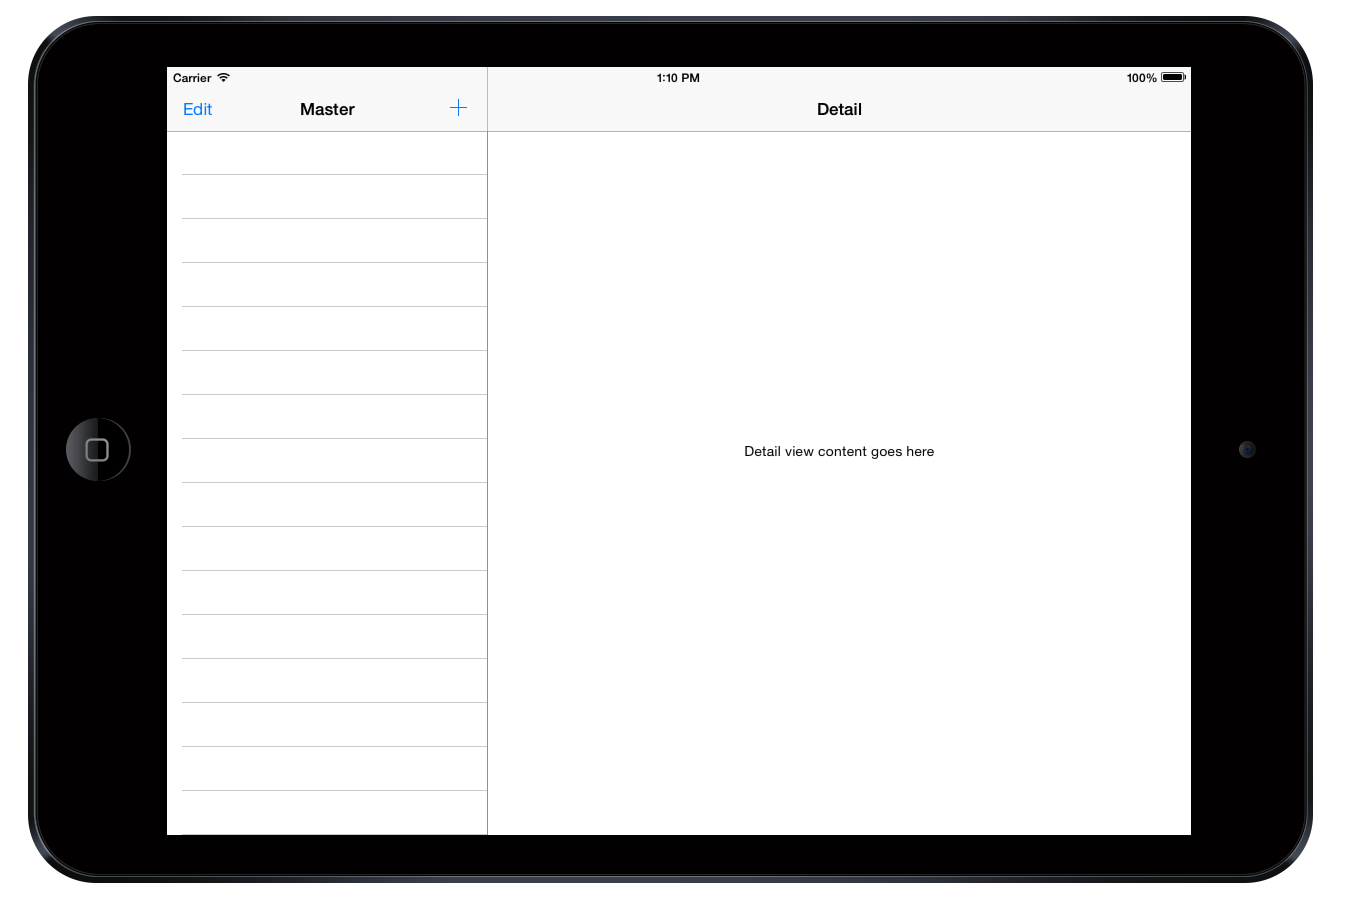
\includegraphics[scale=0.25]{ipad-master-detail-view-controller-mockup}
	\caption{Beispiel einer Master-Detail Applikation auf dem iPad}
	\label{master-detail-view-controller}
\end{figure}

Durch die Verwendung dieses Templates werden die benötigten Klassen, das Datenmodell und die Storyboards direkt generiert. Der \emph{NSManagedContext} des Datenmodels wird in der \emph{AppDelegate} erzeugt und dort an die jeweiligen ViewController weitergegeben, sodass der Zugriff auf das Datenmodell in der gesamten Applikation möglich ist. Alle selbstständig generierten Klassen und Dateien lassen sich selbstverständlich, den eigenen Bedürfnissen nach, verändern und anpassen.

Die geplante Applikation soll mehrere Funktionen abdecken, im Genaueren soll sie es ermöglichen Fingerprints zu sammeln, die gesammelten Fingerprints beziehungsweise Informationen über die Fingerprints anzeigen und eine Positionierung des Geräte im aktuellen Raum ermöglichen.

Dahingehend muss das Storyboard, welches das User Interface repräsentiert dementsprechend angepasst werden.
Dazu kommt ein Tab Bar Controller zum Einsatz, welcher es ermöglicht, mittels einer Tab Bar im unteren Bereich des Bildschirms, zwischen verschiedenen View Controllern auszuwählen. Dies ermöglicht einen schnellen Wechsel zwischen den ViewControllern für das Sammeln der Fingerprints, für die Ausgabe der Informationen über die Fingerprints und für das Anzeigen der aktuellen Position.

\begin{figure}[htb!]
		\centering
	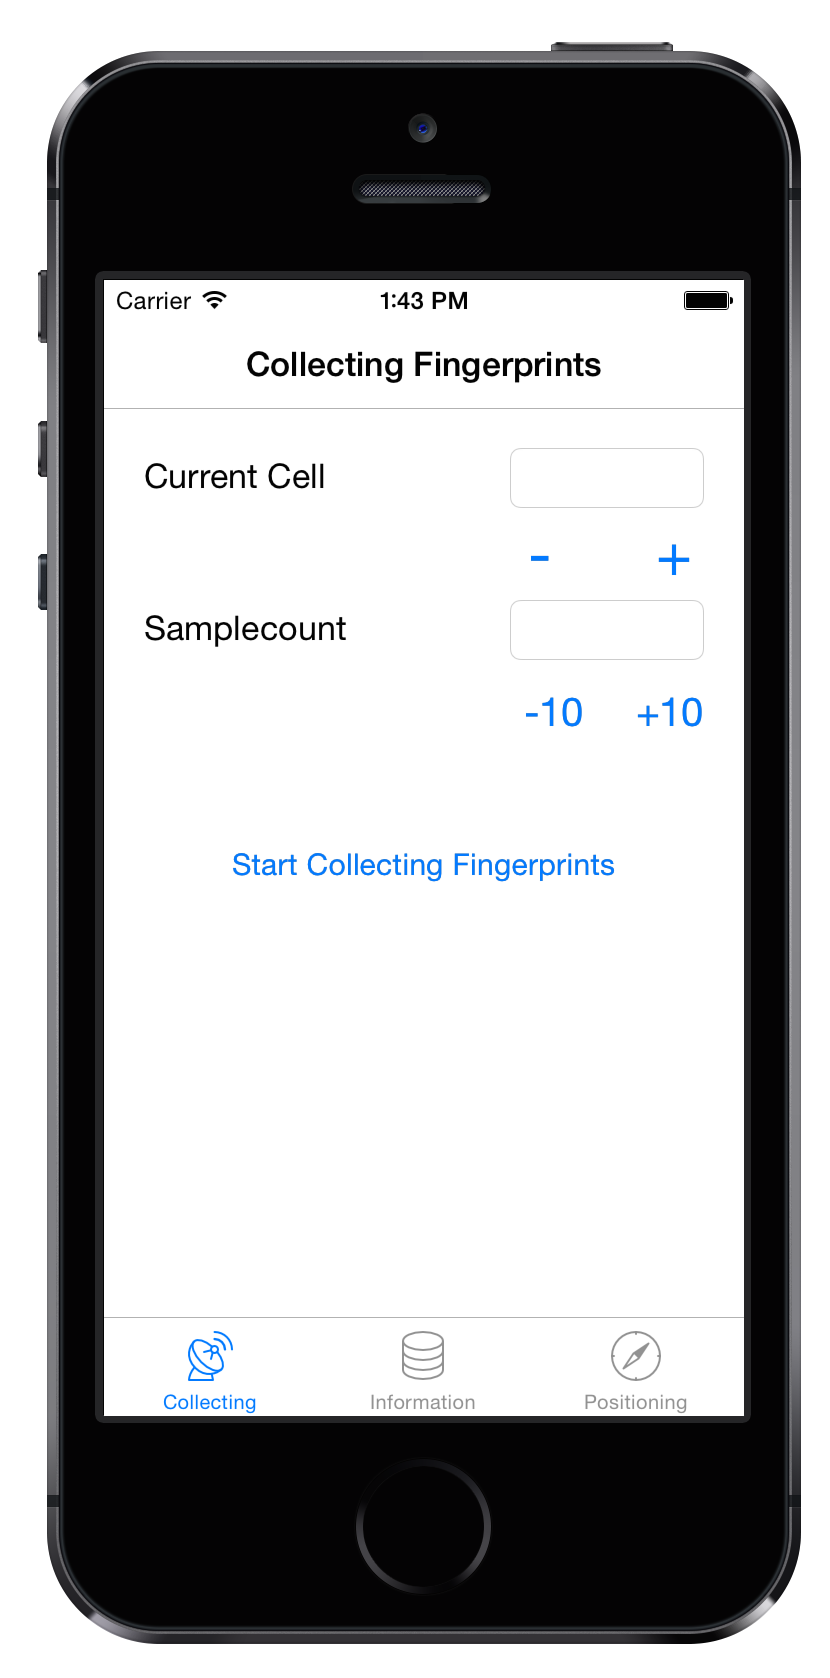
\includegraphics[scale=0.25]{iphone-tab-view-controller-mockup}
	\caption{Beispiel eines TabView Controller auf dem iPhone 5}
	\label{iphone-tab-view-controller}
\end{figure}

%%%%%%%%%%%%%%%%%%%%%%%%%%%%%%%%%%%%%%%%%%%%%%%%%%%%%%%%%%%%
% CoreData Initializing
%%%%%%%%%%%%%%%%%%%%%%%%%%%%%%%%%%%%%%%%%%%%%%%%%%%%%%%%%%%%
Um ein Fingerprinting zu ermöglichen, ist es zunächst wichtig eine geeignete Datenstruktur zur Speicherung der Fingerprints zu erstellen. Hierfür wird das von Apple bereitgestellte CoreData-Framework genutzt, welches einen einfachen Zugriff und Speicherung der Daten ermöglicht. Dazu muss zunächst ein Datenmodell angelegt werden, welches die Entitäten, ihre Attribute und die Beziehungen zwischen den Entitäten beschreibt. Durch die Nutzung des Master-Detail-Templates wurde schon ein Modell erstellt, welches jedoch nur aus einer Entität besteht. Das Modell muss daher für das Figerprinting erweitert werden.

Zunächst werden daher die wichtigsten Eigenschaften eines Fingerprints bestimmt. Diese bestehen aus der aktuellen Position, der empfangenden Signalstärke und dem sendenden Beacon. Daraus lassen sich die grundlegenden Entitäten des Datenmodells bestimmen: \textbf{Beacon}, \textbf{Zelle} und \textbf{Fingerprint}. Des Weiteren ist der Zeitpunkt der Messung relevant und sollte gespeichert werden. Da eine Messung zu einem Zeitpunkt stattfindet und mehrere Fingerprints enthält bietet es sich an, für eine Messung eine eigene Entität zu erstellen, welche einen Zeitstempel enthält und eine Beziehung zu den Fingerprints der Messung besitzt. 
Dieses Modell lässt sich durch den in Xcode integrierten CoreData-Modell-Editor erstellen und das fertige Modell ist in Abbildung \ref{core-data-model-basic} zu sehen.

\begin{figure}[htb!]
		\centering
	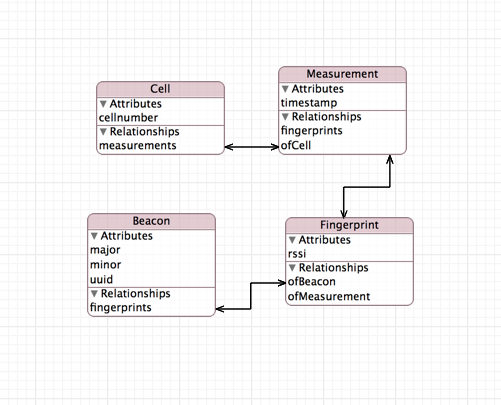
\includegraphics[scale=0.5]{core-data-model-basic}
	\caption{CoreData-Modell im grafischen Editor}
	\label{core-data-model-basic}
\end{figure}

Die Beziehungen zwischen den einzelnen Entitäten lassen sich hier ebenfalls erstellen und bearbeiten. In diesem Modell besteht jeweils zwischen Beacon und Fingerprints, zwischen Messung und Fingerprints und zwischen Messung und Zelle eine \emph{One-to-Many} Beziehung. Dabei beinhaltet eine Messung mehrere Fingerprints, eine Zelle mehrere Messungen und ein Beacon ebenfalls mehrere Fingerprints.

Nachdem dieses Modell erstellt wurde, ist es zusätzlich möglich, für jede Entität eine eigene Klasse zu generieren. Dieses vereinfacht die Handhabung und den Zugriff auf die Attribute, da nicht mit einem generischen \emph{NSManagedObject} gearbeitet werden muss. Die generierten Klassen enthalten alle Attribute der Entitäten in Form von Properties. Bei \emph{To-Many} Beziehungen zu anderen Entiäten werden zusätzlich Methoden zum Hinzufügen und Entfernen dieser Entitäten erstellt.

\begin{listing}[htb!]
	\insertminted{objc}{code_examples/Cell.h}
	\caption{Generierte Klasse für die Zelle im CoreData-Modells}
	\label{lst:cell_objc}
\end{listing}
  

%%%%%%%%%%%%%%%%%%%%%%%%%%%%%%%%%%%%%%%%%%%%%%%%%%%%%%%%%%%%
% ViewController for the diffent purposes
%%%%%%%%%%%%%%%%%%%%%%%%%%%%%%%%%%%%%%%%%%%%%%%%%%%%%%%%%%%%
\textbf{Sammeln der Fingerprints}
Die erste Aufgabe der Applikation ist das Sammeln der aktuellen Fingerprints an einem festgelegten Ort. Dieser Zweig der Applikation setzt sich aus zwei ViewControllern zusammen. Zunächst wird ein ViewController für die Konfiguration der aktuellen Zelle benötigt. In diesem lassen sich etwa der Ort oder die gewünschte Anzahl an Fingerprints bestimmen. Ausserdem ist es möglich weitere Einstellungsmöglichkeiten bereitzustellen, wie etwa die manuelle Festlegung des zu suchenden UUID oder Major-Wertes. 

%%%%%%%%%%%%%%%%%%%%%%%%%%%%%%%%%%%%%%%%%%%%%%%%%%%%%%%%%%%%
% figure of diffenent collecting configuration view controller
%%%%%%%%%%%%%%%%%%%%%%%%%%%%%%%%%%%%%%%%%%%%%%%%%%%%%%%%%%%%
\begin{figure}[h!]
	\centering
	\begin{minipage}[t]{5cm}
		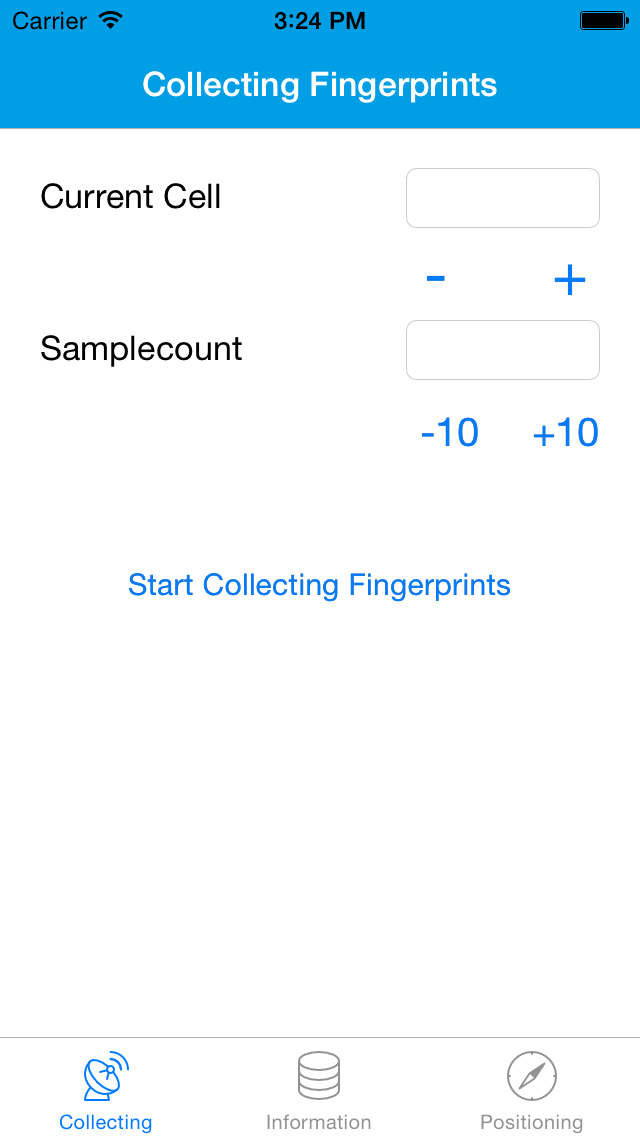
\includegraphics[scale=0.2]{collect-fingerprints-simple}
		\caption{ViewController für einfache Konfiguration.}
		\label{collect-fingerprints-simple}
	\end{minipage}
	\hspace{2cm}
	\begin{minipage}[t]{5cm}
			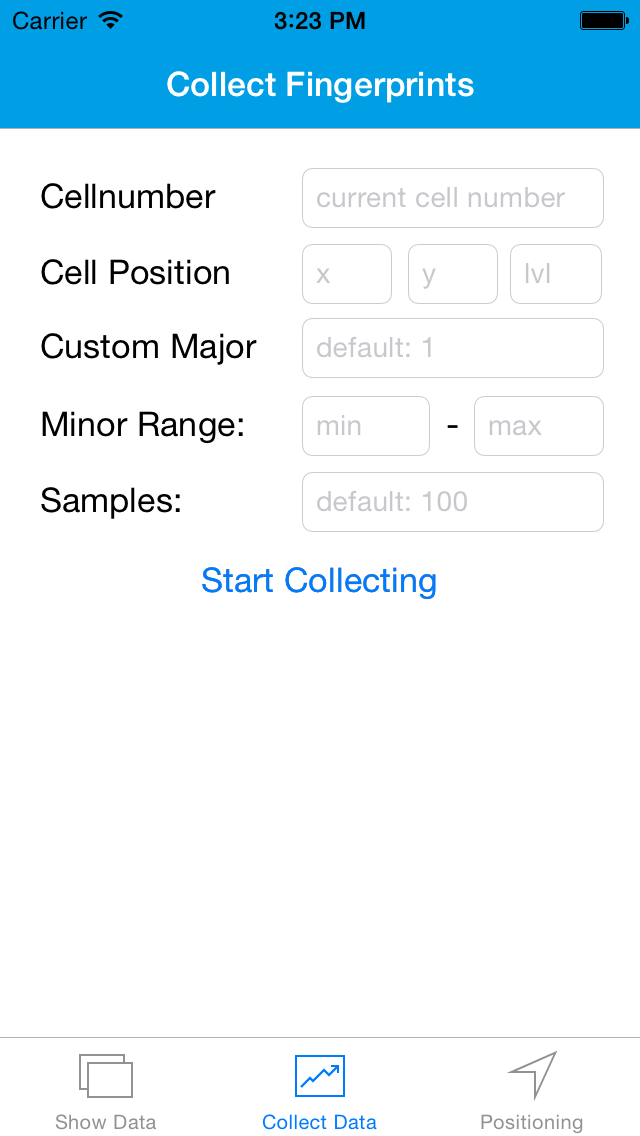
\includegraphics[scale=0.2]{collect-fingerprints-detailed}
			\caption{ViewController mit mehreren Konfigurationsmöglichkeiten.}
			\label{collect-fingerprints-detailed}
	\end{minipage}
		\caption{Mögliche ViewController für die Konfiguration des Fingerprinting}
		\label{collect-fingerprints}
\end{figure}

Nachdem alle benötigten Daten für die Konfiguration eingegeben wurden, sollen nun die Fingerprints gesammelt werden.

Dazu muss ein weiterer ViewController angelegt werden. In diesem wird ein \emph{CLLocationManager}-Objekt angelegt, welcher für den Empfang der Beacon-Daten zuständig ist. Nachdem dieser erstellt und initialisiert wurde, wird der ViewController als \emph{delegate} des CLLocationManagers gesetzt.

\begin{listing}[htb!]
    \insertminted{objc}{code_examples/locationManager.m}
    \caption{Beispielinitialisierung für einen LocationManager.}
    \label{lst:locationmanager_objc}
\end{listing}

Dies ermöglicht dem CLLocationManger dem aktuellen ViewController eine Rückmeldung zu geben, sobald dieser Beacons in der zuvor spezifizierten Region gefunden hat. Dies erfolgt durch die Implementierung der Methode \emph{didRangeBeacons:inRegion}, welche vom CLLocationManager aufgerufen wird, sobald dieser auf Beacons in der Region geprüft hat. Diese Methode erhält dabei ein Array mit \emph{CLBeacon}-Objekten, welche die empfangenden Beacon-Informationen enthalten. 

Für die Suche nach den Beacons muss außerdem die zu suchende Region spezifiziert werden. Dazu wird ein \emph{CLBeaconRegion}-Objekt erstellt, welcher die Informationen einer Region enthält. Dazu zählen zum Beispiel der UUID und der Identifier der Region. Dies sind die beiden zwingend notwendigen Angaben. Darüberhinaus lässt sich zudem der Major-Wert festlegen, nach dem gesucht werden soll. Eine weitere Möglichkeit ist es nur nach Beacons mit bestimmtem UUID, Major und Minor-Wert zu suchen.
In dieser Applikation wird die CLBeaconRegion nur mittels UUID und Identifier initialisiert, da nur eine Region für die Messung benötigt wird.

Die Suche nach den Beacons wird dabei mit der \emph{startRangingBeaconsInRegion:} Methode des CLLocationManagers gestartet.

Nach dem Start, wird die \emph{didRangeBeacons:inRegion}-Methode periodisch aufgerufen und erhält dabei die zurzeit in Reichweite befindlichen Beacons, welche mit der spezifizierten Region übereinstimmen.
Das Array beinhaltet dabei \emph{CLBeacon} Objekte, welche ein gefundenes Beacon repräsentieren.

Für das Fingerprinting müssen nun die gefundenen Beacons in das Datenmodell gespeichert werden. Dies geschieht über eine selbstgeschriebene Methode, welche über alle gefundenen Beacons iteriert und diese, unter Berücksichtigung der aktuellen Zelle, zum Datenmodell hinzufügt. Diese Methode wird in der \emph{didRangeBeacons:inRegion}-Methode ausgeführt, welche vom \emph{CLLocationManager} aufgerufen wird.

\begin{listing}[htb!]
    \insertminted{objc}{code_examples/didRangeBeacons.m}
    \caption{Beispiel der \emph{didRangeBeacons:inRegion}-Methode}
    \label{lst:didRangeBeacons_objc}
\end{listing}

Während der Aufzeichnung der Fingerprints wird eine Fortschrittsanzeige und die aktuelle Anzahl der in Reichweite liegenden Beacons angezeigt, wie auf Abbildung \ref{collecting-view-controller} zu erkennen.

\begin{figure}[htb!]
		\centering
	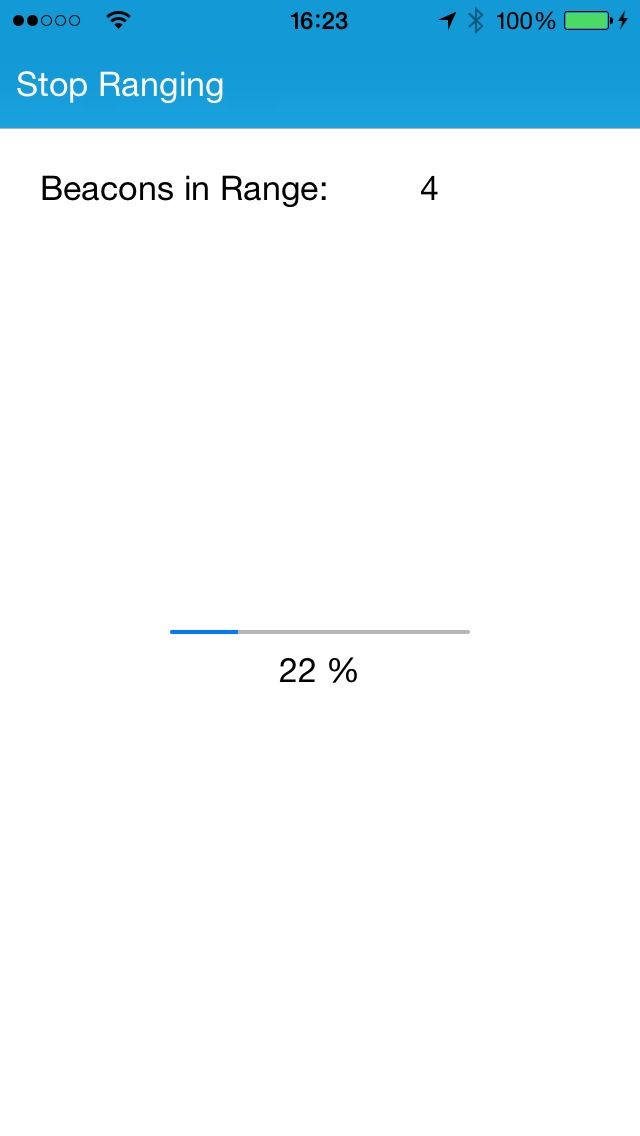
\includegraphics[scale=0.3]{collecting-view-controller}
	\caption{Anzeige während des Sammelns von Fingerprints}
	\label{collecting-view-controller}
\end{figure}

%%%%%%%%%%%%%%%%%%%%%%%%%%%%%%%%%%%%%%%%%%%%%%%%%%%%%%%%%%%%
% Presenting ViewController
%%%%%%%%%%%%%%%%%%%%%%%%%%%%%%%%%%%%%%%%%%%%%%%%%%%%%%%%%%%%
\textbf{Ausgabe der Fingerprints}
Der vom Template generierte Master-Detail-ViewController wird verwendet um die gesammelten Fingerprints zu verwalten. Dabei wird der Tabellen-View (Master) genutzt um die bisher aufgezeichneten Zellen anzuzeigen. Bei einem Klick auf die jeweilige Tabellenspalte der Zelle lassen sich zusätzliche Informationen ausgeben.
Ausserdem wurde eine Übertragung der gesammelten Daten an einen Server implementiert. Dazu werden die Daten in das \emph{json}-Format überführt und dann an einen lokalen Server geschickt, welcher mittels \emph{Node.js} programmiert wurde. Dieser Server empfängt die Datei und speichert sie anschließend auf die Festplatte. 
Dies ermöglicht eine einfache Auswertung der gesammelten Daten.


%%%%%%%%%%%%%%%%%%%%%%%%%%%%%%%%%%%%%%%%%%%%%%%%%%%%%%%%%%%%
% Positioning ViewController
%%%%%%%%%%%%%%%%%%%%%%%%%%%%%%%%%%%%%%%%%%%%%%%%%%%%%%%%%%%%
\textbf{Positionsbestimmung}
Für die Bestimmung der aktuellen Position ist die aktuelle Zelle der wichtigste Wert. Die Ausgabe einer Karte mit der aktuellen Position ist zwar hilfreich für eine praktische Anwendung, für das Testen jedoch nicht notwendig.
Für die Positionsbestimmung werden, wie schon beim Sammeln der Fingerprints, zunächst aktuelle Werte der Beacons benötigt. Die Konfiguration und Initialisierung des \emph{CLLocationManagers} und der \emph{CLBeaconRegion} ist dabei identisch zu der Vorgehensweise des Fingerprinting-ViewControllers.

Statt die erhaltenen Beacon-Daten jedoch in die Datenbank zu übernehmen, werden diese direkt weiterverarbeitet. Dazu werden verschiedene Positionierungsalgorithmen angewandt, auf welche im Kapitel \ref{sec:implementation:fingerprinting:positioning} genauer eingegangen wird. 
Diese Algorithmen liefern nun die, nach den Berechnungen, am nächsten liegende Zelle zurück. Der ViewController kümmert sich dann um die Ausgabe der Zellennummer auf dem Bildschirm.


%%%%%%%%%%%%%%%%%%%%%%%%%%%%%%%%%%%%%%%%%%%%%%%%%%%%%%%%%%%%
\section{Ansatz zur Positionsbestimmung}
\label{sec:implementation:positioning}
%%%%%%%%%%%%%%%%%%%%%%%%%%%%%%%%%%%%%%%%%%%%%%%%%%%%%%%%%%%% 
Bei der Positionsbestimmung geht es um die Bestimmung des aktuellen Ortes in Echtzeit und das auf bis zu wenige Meter genau. Bei der Positionsangabe handelt es sich hier um eine zweidimensionale Position, da dies für die Indoor-Positionierung ausreichend ist.

Bei der Positionsbestimmung wurden zwei verschiedene Ansätze untersucht. Zum einen die Trilateration, welche eine Positionierung mittels Entfernungen zu verschiedenen Fixpunkten ermöglicht und zum Anderen die Positionierung mittels Fingerprinting, welches eine Datenbank mit sogenannten Fingerprints, also vorher aufgezeichneten Messwerten und damit verbundenen Positionsdaten, voraussetzt und über diese Daten die aktuelle Position bestimmt.

Die Positionsbestimmung soll dabei in einem 2D-Raum erfolgen, da die Höhe vernachlässigt werden kann. In der realen Welt kann die Höhe ebenfalls vernachlässigt werden, da dort Stockwerke meist einen deutlichen Höhenunterschied aufweisen, sodass dieser Höhenunterschied über andere Faktoren eindeutig bestimmt werden kann.


%%%%%%%%%%%%%%%%%%%%%%%%%%%%%%%%%%%%%%%%%%%%%%%%%%%%%%%%%%%%
\section{Trilateration}
\label{sec:implementation:trilateration}
%%%%%%%%%%%%%%%%%%%%%%%%%%%%%%%%%%%%%%%%%%%%%%%%%%%%%%%%%%%%
Die Trilateration ist eine Methode zur Bestimmung der aktuellen Position. Im Gegensatz zur Triangulation, welche die Position anhand der Winkelgrößen zwischen verschiedenen Fixpunkten bestimmt, wird bei der Trilateration die Position durch die Abstände zu den Fixpunkten bestimmt. 

Die Trilateration macht sich dabei zunutze, dass sich ein Objekt, bei gegebenem Abstand zum Fixpunkt, auf einer Kreisbahn um diesen befinden muss, wobei der Radius des Kreises dem Abstand entspricht. Um nun einen genauen Standpunkt zu bestimmen, sind mindestens drei Fixpunkte und die dazugehörige Abstände nötig, da so im zweidimensionalem Raum ein eindeutiger Schnittpunkt entsteht.

\begin{figure}[htb!]
	\centering
	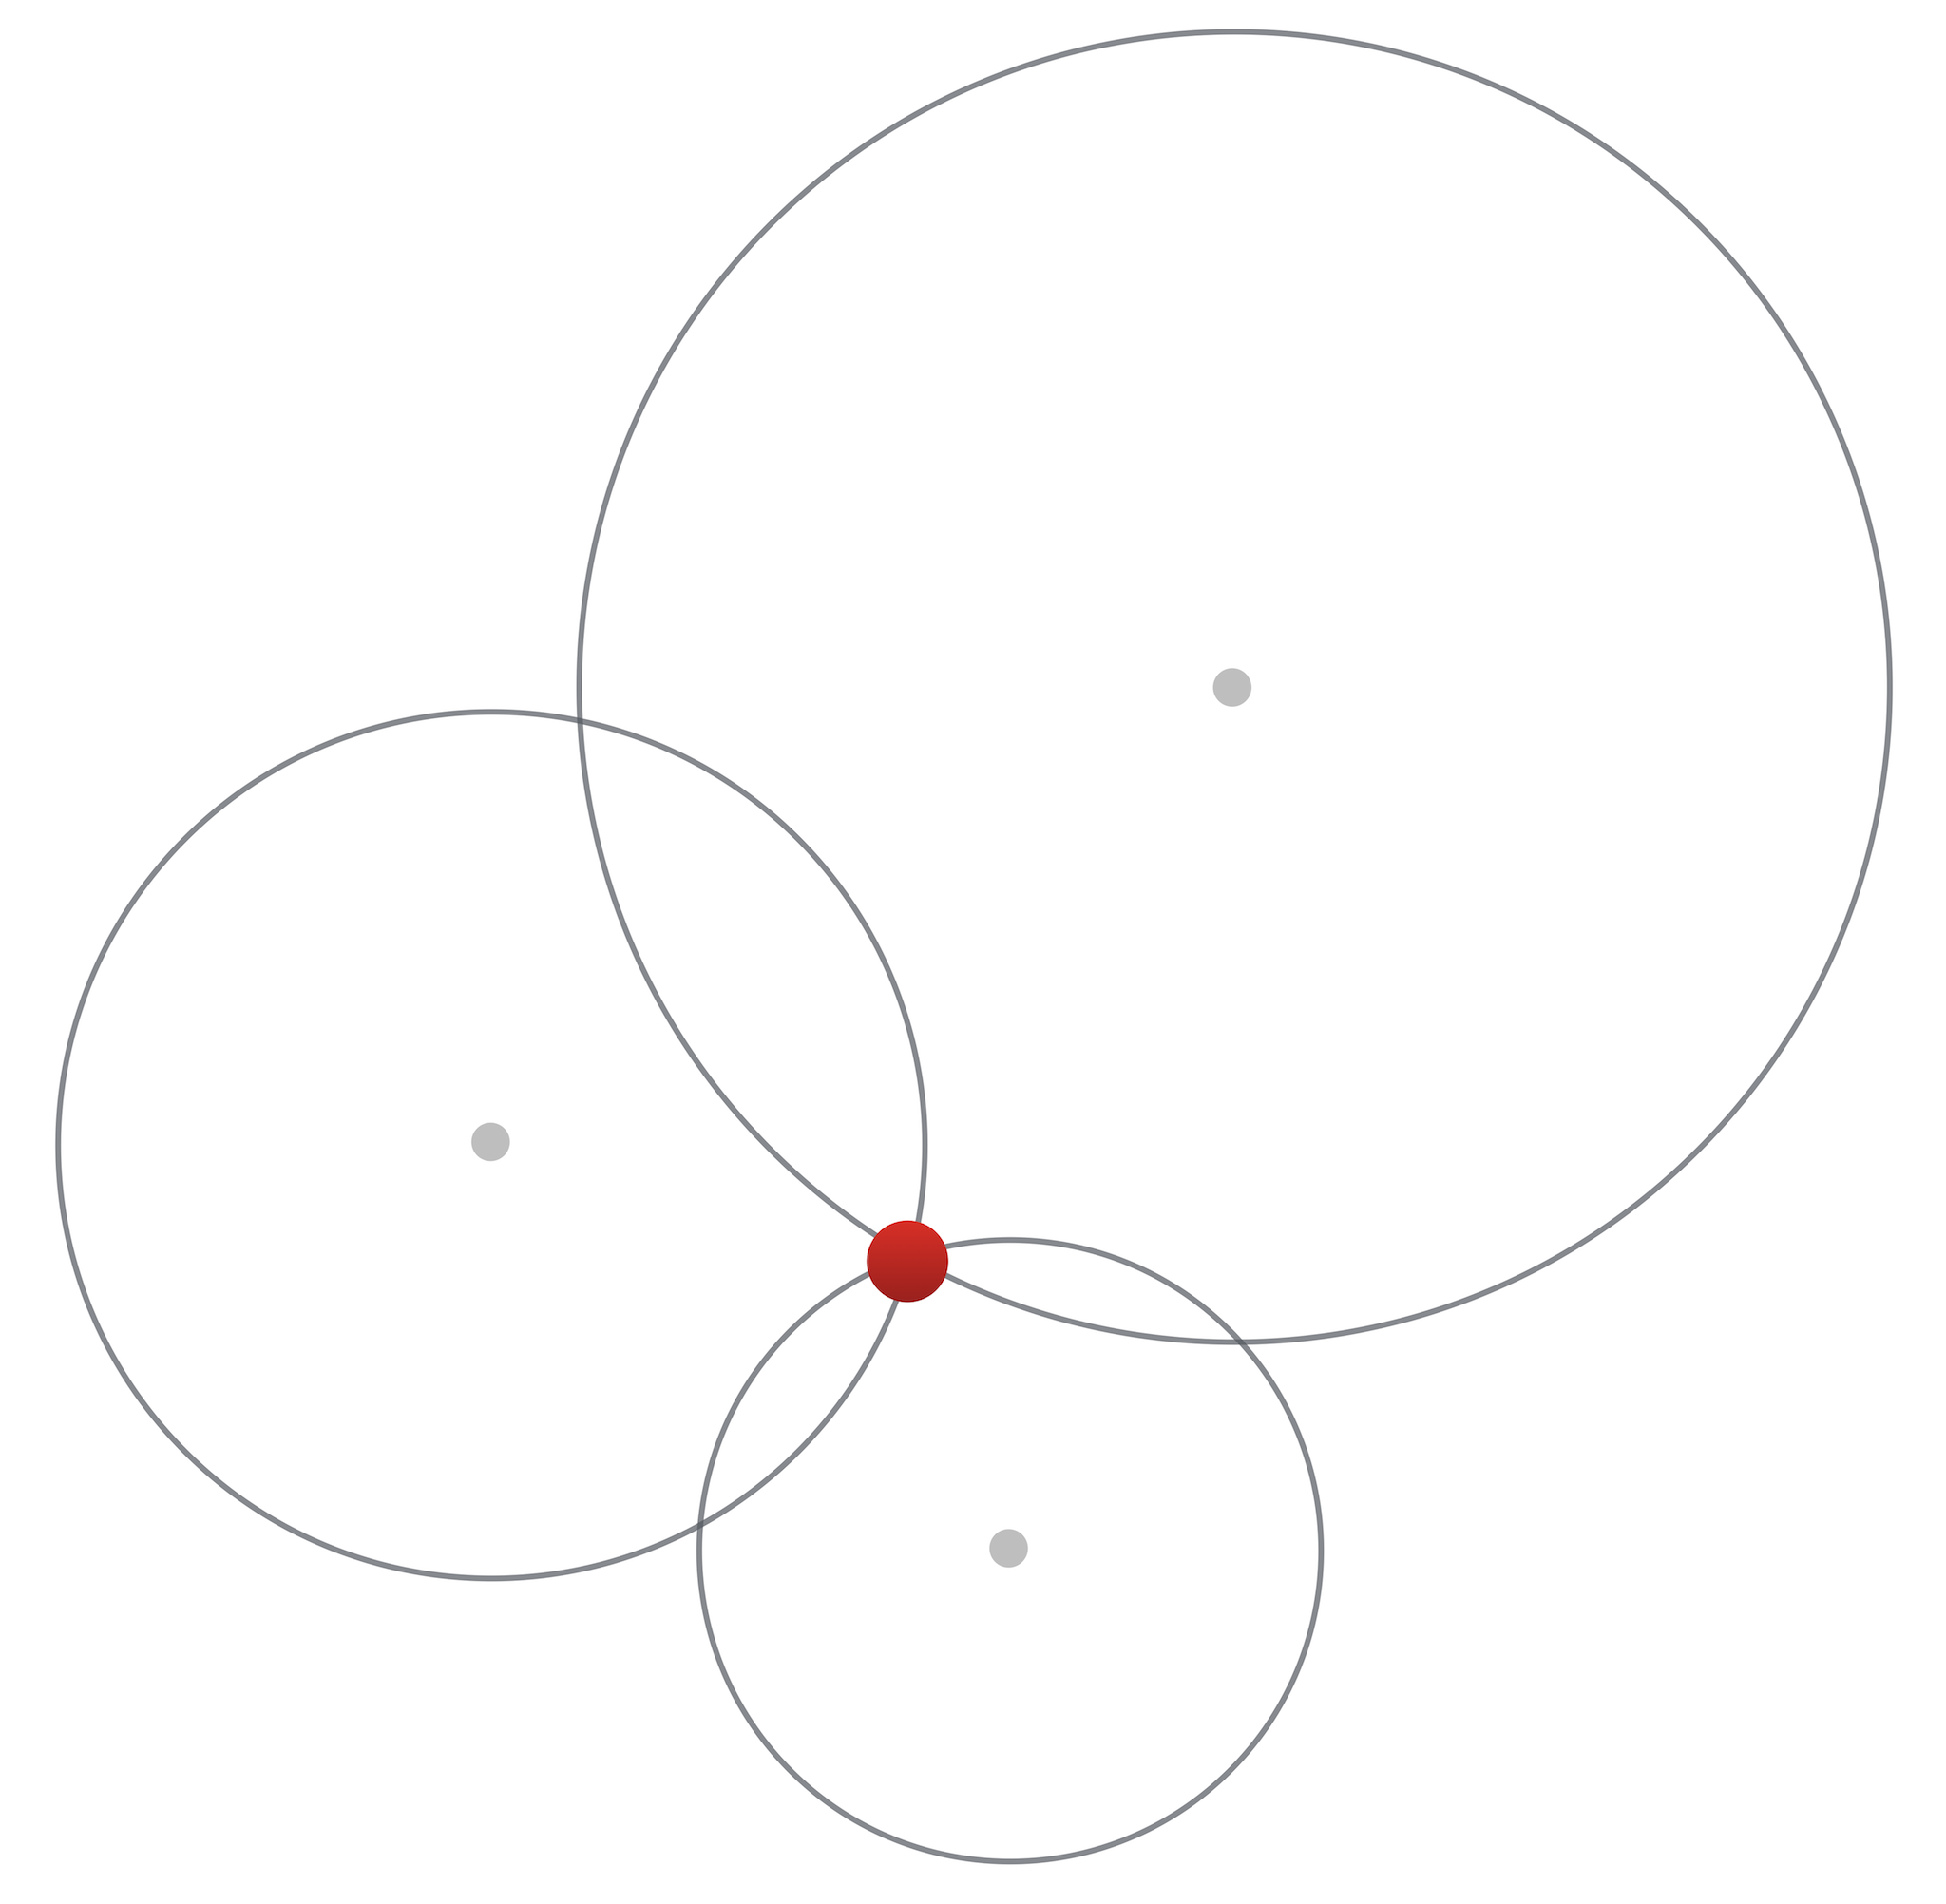
\includegraphics[scale=1.5]{trilateration}
	\caption{Funktionsprinzip der Trilateration}
	\label{trilateration-accurate}
\end{figure}

In Abbildung \ref{trilatertion-accurate} sieht man dabei die Funktionsweise der Trilateration bei genauer Abstandsbestimmung. In realen Messungen und Positionsbestimmungen ist es jedoch nicht möglich genaue Abstände zu bestimmen, da es immer zu Messungenauigkeiten kommen kann.
Bei solchen ungenauen Messungen ist es nun nicht mehr möglich einen genauen Schnittpunkt zu finden. 

Um diese Ungenauigkeit auszugleichen wird das Verfahren entsprechend angepasst. Dabei werden Geraden durch die Schnittpunkte der einzelnen Umkreise gelegt. Dadurch entsteht zwischen den Geraden ein neuer Schnittpunkt, welcher die aktuelle Position repräsentiert. Dieses Verfahren wird in Abbildung \ref{trilateration-inaccurate} dargestellt.

\begin{figure}[htb!]
		\centering
	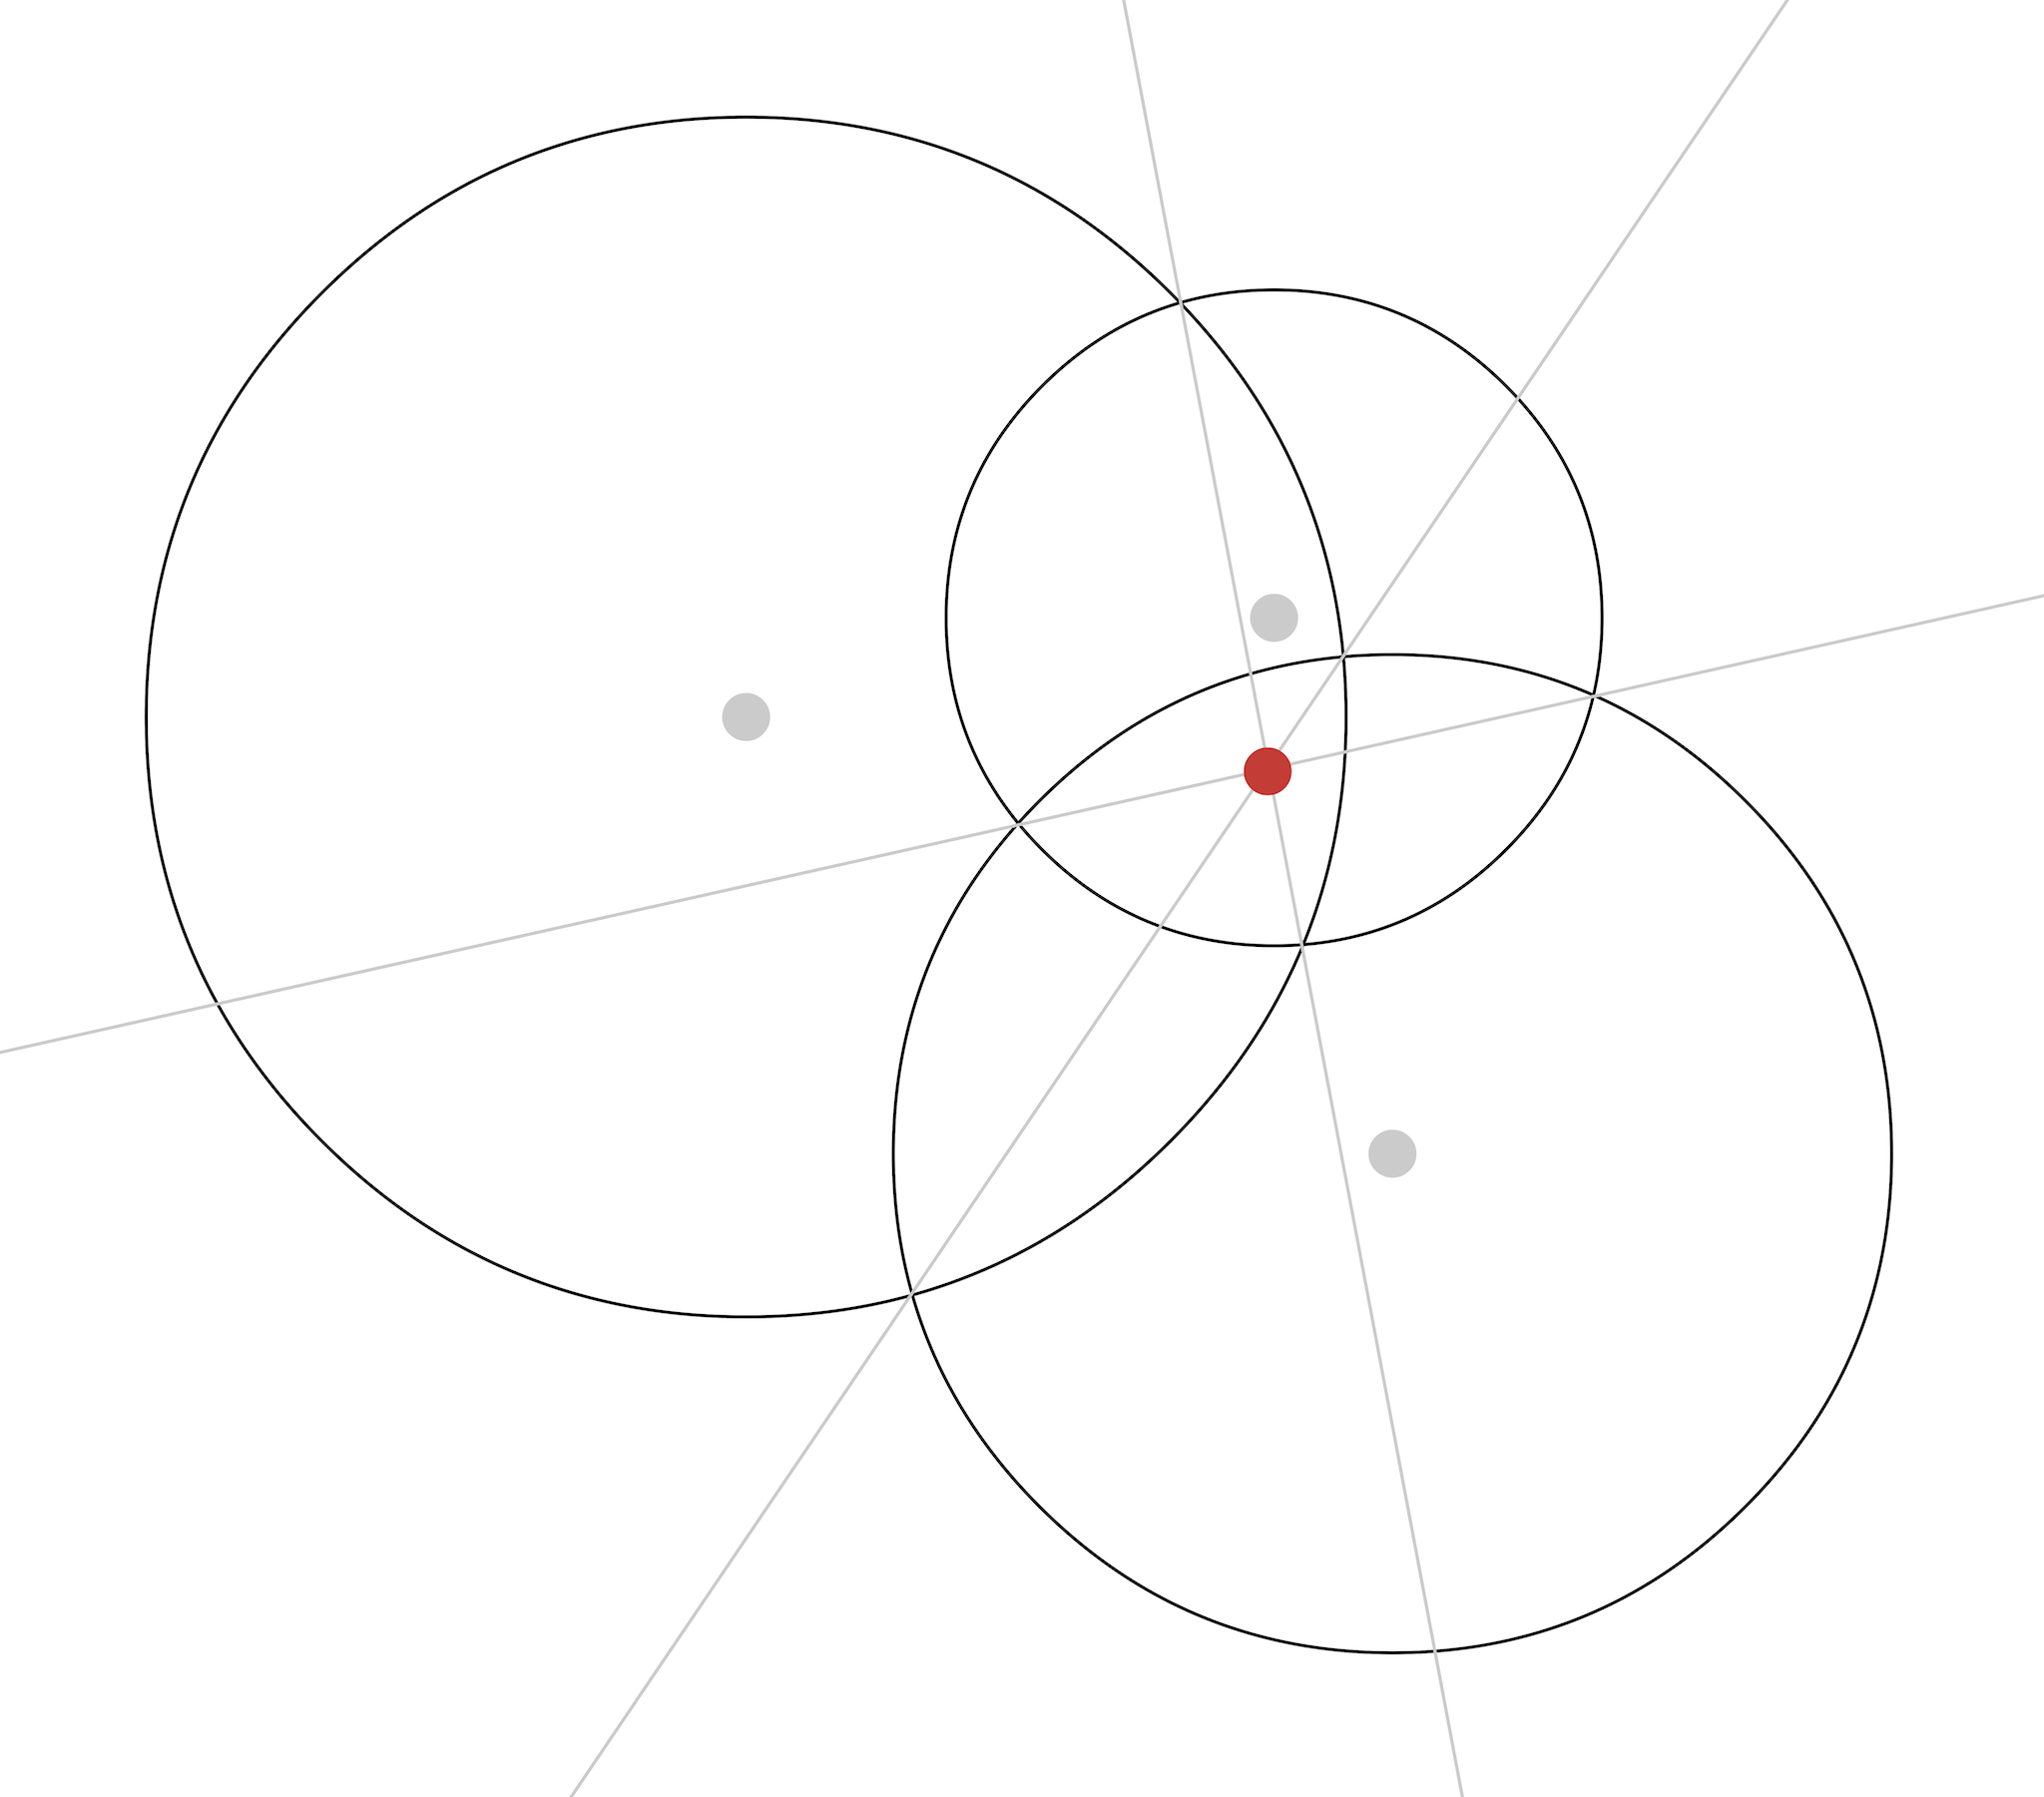
\includegraphics[scale=1.5]{trilateration-inaccurate}
	\caption{Trilateration bei ungenauen Abständen zu den Fixpunkten}
	\label{trilateration-inaccurate}
\end{figure}

Damit ist es möglich auftretende Ungenauigkeiten zu kompensieren und trotzdem eine genaue Positionsbestimmung durchzuführen.

Bei der genutzten iBeacons beziehungsweise Bluetooth-Technologie ist eine genaue Entfernungsangabe jedoch nicht vorgesehen, wodurch das Verfahren der Trilateration nicht direkt angewandt werden kann. Dafür muss zunächst ein Ersatzindikator für die Entfernungsmessung bestimmt werden.
Bei der Bluetooth-Technologie bietet sich dafür die Signalstärke an.
Dabei wird die Tatsache genutzt, dass die Signalstärke mit zunehmendem Abstand sinkt und man somit aus der aktuellen Signalstärke auch die aktuelle Entfernung bestimmen kann. 
Das Verhältnis zwischen Entfernung und Signalstärke bei elektromagnetischen Wellen wird durch das Abstandsgesetz beschrieben, welches besagt, das die Signalstärke quadratisch zum Abstand abnimmt.

\begin{equation}
	\text{\emph{Signalstärke}} = \frac{\text{\emph{Ausgangssignalstärke}}}{\text{\emph{Entfernung}}^2}
\end{equation}

Diese Annahme mag bei freien Flächen korrekt sein, in Innenräumen kommen jedoch weitere Faktoren hinzu. 
Durch Wände und Hindernisse im Raum, wie zum Beispiel Schränke, Regale, usw., kommt es dort zu einer Dämpfung des Signals, wodurch die Signalstärke beeinflusst wird. Des Weiteren kann es in Innenräumen auch zu Streuung und Reflexionen kommen, welche das Signal zusätzlich verfälschen.

Diese Annahme bestätigt sich auch bei den Messungen. Diese zeigen, dass die gemessene Signalstärke nicht, wie angenommen, mit der Entfernung stetig abnimmt, sondern sehr stark schwankt, wodurch keine genaue Entfernungsbestimmung durchgeführt werden kann.

Die Methode der Trilateration wurde auf Grund der fehlenden Genauigkeit verworfen. 

%%%%%%%%%%%%%%%%%%%%%%%%%%%%%%%%%%%%%%%%%%%%%%%%%%%%%%%%%%%%
\section{Fingerprinting}
\label{sec:implementation:fingerprinting}
%%%%%%%%%%%%%%%%%%%%%%%%%%%%%%%%%%%%%%%%%%%%%%%%%%%%%%%%%%%%
Das Fingerprinting ist ein Verfahren der Positionsbestimmung auf der Grundlage von zuvor erhobenen Messwerten, den sogenannten Fingerprints.
Die Funktionsweise des Fingerprintings unterscheidet sich grundlegend von der Methode der Trilateration, da hierbei keine direkte Berechnung der Position über Entfernungsgrößen geschieht, sondern die Positionierung über, in einer Datenbank abgelegte, Erfahrungswerte geschieht.

Um dieses Verfahren umzusetzen muss der Messraum, in welchem die Positionierung statt finden soll, zunächst in ein Gitternetz eingeteilt werden, wobei jede Zelle des Gitters eine mögliche Position im Raum repräsentiert. Die Größe dieser Zellen ist prinzipiell frei wählbar, wird jedoch im Wesentlichen durch zwei Faktoren bestimmt. 
Zum einen die gewünschte Genauigkeit, da jede Zelle eine mögliche Position repräsentiert. Dabei wird durch die Größe der Zellen auch die Genauigkeit der Position bestimmt. Daraus erschließt sich, dass die Genauigkeit zunimmt, wenn die Zellengröße verkleinert wird.
Der zweite Faktor bei der Wahl der Zellengröße, ist die eindeutige Bestimmung einer Zelle. Dies ist darauf zurückzuführen, dass bei kleineren Zellen die Differenzen zwischen den einzelnen Zellen ebenfalls abnehmen. Um nun eine genaue Bestimmung einer spezifischen Zelle zu ermöglichen, sollte jede Zelle so groß gewählt werden, dass dies noch möglich ist.

Anhand dieser zwei Kriterien sollte die Zellengröße so gewählt werden, dass eine gute Unterscheidbarkeit zwischen den einzelnen Zellen gewährleistet ist und trotzdem eine möglichst genaue Positionsbestimmung erzielt werden kann.


Nachdem die Zellengröße ausgewählt wurde, müssen nun die Fingerprints erhoben wernde.
Das Fingerprintingverfahren besteht dabei im Wesentlichen aus zwei Phasen.

Die erste Phase ist die sogenannte \emph{Trainingsphase} (auch Offline-Phase). Dabei werden die \emph{Fingerprints} gesammelt, welche letztlich zur Positionsbestimmung genutzt werden. 
In der Trainingsphase werden daher für jede Zelle des Messraumes eine Reihe von Fingerprints gesammelt. Die Anzahl der Fingerprints sollte dabei so groß sein, dass Messfehler kompensiert werden können. 
Ein Fingerprint kann sich dabei aus verschiedenen Daten zusammensetzen. 
In diesem Fall besteht ein Fingerprint aus der aktuellen Zellennummer beziehungsweise den Zellenkoordinaten, einem Zeitstempel mit aktuellem Datum und Uhrzeit und den Signalstärken zu den verschiedenen, in Reichweite befindlichen Sendestationen, welches in diesem Fall die Beacons sind.

Die Sammlung der Fingerprints muss für jede Zelle geschehen und macht die Trainingsphase daher sehr zeitaufwendig. 

In der zweiten Phase, auch \emph{Onlinephase} genannt, werden die zuvor gesammelten Informationen verwendet um die aktuelle Position zu bestimmen. 
Dafür werden die gesammelten Fingerprints mit den aktuell gemessenen Signalstärken verglichen. Wenn eine Übereinstimmung gefunden wird, wird die Position des passenden Fingerprints als aktuelle Position angenommen.

\todo{Einfügen von Zeichnung welche Zellen und Fingerprints verdeutlicht}

%%%%%%%%%%%%%%%%%%%%%%%%%%%%%%%%%%%%%%%%%%%%%%%%%%%%%%%%%%%%
\subsection{Sammlung und Speicherung von Fingerprints}
\label{sec:implementation:fingerprinting:collecting}
%%%%%%%%%%%%%%%%%%%%%%%%%%%%%%%%%%%%%%%%%%%%%%%%%%%%%%%%%%%%
Um eine Positionierung mittels Fingerprinting zu ermöglichen, ist es zunächst nötig einen grundlegenden Datensatz mit Fingerprints zu sammeln, welcher später für die Positionsbestimmung genutzt werden kann. Dazu ist es wichtig zu bestimmen, welche Informationen benötigt werden.

Für jeden Fingerprint muss dabei die aktuelle Position der Messung, das zugehörige Beacon und die aktuelle Signalstärke zwingend vorhanden sein.
Zusätzlich ist es sinnvoll den aktuellen Zeitpunkt der Messung zu speichern, um so, wenn nötig, veraltete Fingerprints zu entfernen. 

Für das iOS-Programm lag es daher nahe, ein CoreData-Datenmodell anzulegen und die Speicherung der Daten darüber abzuwickeln.
Dafür wurden diverse Entitäten angelegt:

Beacon:
	\begin{quote}Repräsentiert ein Beacon und beinhaltet UUID, Major und Minor-Wert\end{quote}
Cell:
	\begin{quote}Repräsentiert eine Zelle und beinhaltet die Zellennummer\end{quote}
Fingerprint:
	\begin{quote}Repräsentiert einen Fingerprint eines Beacons und beinhaltet die gemessene Signalstärke\end{quote}
Measurement:
	\begin{quote}Repräsentiert eine Messung von Fingerprints und beinhaltet den Zeitstempel des Zeitpunktes der Messung\end{quote}

Untereinander verfügen die Entitäten über diverse Beziehungen, sodass jeder Fingerprint eindeutig einer Zelle und einem Beacon zuzuordnen ist.

%%%%%%%%%%%%%%%%%%%%%%%%%%%%%%%%%%%%%%%%%%%%%%%%%%%%%%%%%%%%
\subsection{Positionsbestimmung}
\label{sec:implementation:fingerprinting:positioning}
%%%%%%%%%%%%%%%%%%%%%%%%%%%%%%%%%%%%%%%%%%%%%%%%%%%%%%%%%%%%
Bei der Positionsbestimmung mittels Fingerprinting gibt es verschiedene Ansätze.
Das erste Verfahren vergleicht alle Fingerprints in der Datenbank mit den aktuellen Messwerten und bestimmt damit die aktuelle Position.
Eine weitere Möglichkeit besteht darin, den Durchschnittswert der Fingerprints zu bilden um diesen dann mit den aktuellen Werten zu vergleichen.
Die letzte untersuchte Möglichkeit ist die der Wahrscheinlichkeitsverteilung der Werte. Hier wird über die Wahrscheinlichkeitswerte der einzelnen Messwerte die aktuelle Position bestimmt.

%%%%%%%%%%%%%%%%%%%%%%%%%%%%%%%%%%%%%%%%%%%%%%%%%%%%%%%%%%%%
\subsection{Einfache Positionsbestimmung mittels Nearest-Neighbor-Verfahren}
\label{sec:implementation:fingerprinting:positioning:naiv}
%%%%%%%%%%%%%%%%%%%%%%%%%%%%%%%%%%%%%%%%%%%%%%%%%%%%%%%%%%%%

%%%%%%%%%%%%%%%%%%%%%%%%%%%%%%%%%%%%%%%%%%%%%%%%%%%%%%%%%%%%
\subsubsection{Algorithmus}
\label{sec:implementation:fingerprinting:positioning:naiv:algorithm}
%%%%%%%%%%%%%%%%%%%%%%%%%%%%%%%%%%%%%%%%%%%%%%%%%%%%%%%%%%%%

Bei der einfachen und naiven Bestimmung der aktuellen Position, werden alle zuvor gesammelten Fingerprints mit den aktuell gemessenen Signalstärken verglichen. Dies führt dazu, dass bei größeren Fingerprint-Datenbanken auch die Rechenzeit und der Energieverbrauch steigt. 

Bei dem Vergleich der Messwerte mit den gespeicherten Fingerprints wird das Nearest-Neighbor-Verfahren verwendet. Dabei werden sowohl die aktuellen Messwerte, als auch die Fingerprints als Vektoren aus den Signalstärken zusammengefasst und aus diesen Vektoren wird die jeweilige Entfernung der beiden Werte berechnet. Die einzelnen Signalstärken-Werte sind die Werte von allen in Reichweite befindlichen Beacons.

Bei der Berechnung wird dabei für jeden Fingerprint ein Vektor erzeugt, welcher die Signalstärken zu den in Reichweite befindlichen Beacons beinhaltet.
Die Signalstärke für die Beacons wird hier als \emph{FSig} bezeichnet, wobei ein Zusatz angibt auf welches Beacon sich der Wert bezieht, zum Beispiel \emph{FSigB1} für die Signalstärke des Beacons 1.
Die Signalstärke der aktuellen Messung wird mit \emph{MSig} abgekürzt und ebenfalls um den Identifikator des Beacons erweitert.


\begin{equation}
	\begin{pmatrix}
		FSigB1 \\
		FSigB2 \\
		FSigB3 \\
		...
	\end{pmatrix} -
	\begin{pmatrix}
		MSigB1 \\
		MSigB2 \\
		MSigB3 \\
		...
	\end{pmatrix}
	= 
	\begin{pmatrix}
		FSigB1 - MSigB1 \\
		FSigB2 - MSigB2 \\
		FSigB3 - MSigB3 \\
		...
	\end{pmatrix}
\end{equation}

\begin{equation}
	\begin{pmatrix}
		FSigB1 - MSigB1 \\
		FSigB2 - MSigB2 \\
		FSigB3 - MSigB3 \\
		...
	\end{pmatrix}
	=
	\begin{pmatrix}
		Diff1 \\
		Diff2 \\
		Diff3 \\
		...
	\end{pmatrix}
	\widehat{=}
	\sqrt{Diff1^2 + Diff2^2 + Diff3^2 + ...}
\end{equation}

Aus den Differenzen beziehungsweise die Abstände zwischen den einzelnen Signalstärke-Vektoren lässt sich nun der Nearest-Neighbor bestimmen und damit die wahrscheinlichste Position im Raum.


%%%%%%%%%%%%%%%%%%%%%%%%%%%%%%%%%%%%%%%%%%%%%%%%%%%%%%%%%%%%
\subsubsection{Implementierung}
\label{sec:implementation:fingerprinting:positioning:naiv:implementation}
%%%%%%%%%%%%%%%%%%%%%%%%%%%%%%%%%%%%%%%%%%%%%%%%%%%%%%%%%%%%
Bei der Implementierung dieser Methode wird für jedes Set von Fingerprints in der Datenbank die euklidische Distanz zu den aktuell gemessenenen Signalstärken berechnet. Dazu wird über die vorhandenen Messungen iteriert, welche jeweils ein Set von gemessenen Fingerprints zu einem bestimmten Zeitpunkt enthalten. Diese Signalstärken werden in einen Vektor transformiert, sodass die Distanz berechnet werden kann. In Listing \ref{lst:euclidean_distance_objc} sieht man die Berechnung der euklidischen Distanz zweier Vektoren, welche in Form eines Arrays eingelesen werden.

\begin{listing}[htb!]
    \insertminted{objc}{code_examples/euclidean_distance.m}
    \caption{Bestimmung der euklidischen Distanz zwei Vektoren}
	\label{lst:euclidean_distance_objc}
\end{listing}

Die Messung mit der geringsten euklidischen Distanz wird dabei gespeichert, sodass diese, nachdem alle Measurements durchiteriert wurden, zurückgegeben werden kann. Anhand dieser Messung lässt sich nun die zugehörige Zelle bestimmen und ausgeben.

%%%%%%%%%%%%%%%%%%%%%%%%%%%%%%%%%%%%%%%%%%%%%%%%%%%%%%%%%%%%
\subsubsection{Probleme}
\label{sec:implementation:fingerprinting:positioning:naiv:problems}
%%%%%%%%%%%%%%%%%%%%%%%%%%%%%%%%%%%%%%%%%%%%%%%%%%%%%%%%%%%%
Bei dem Standard Nearest-Neighbor-Verfahren kommt es jedoch zu einigen Problemen. 
Die Masse der zu überprüfenden Daten kann, je nach der Größe der Fingerprint-Datenbank, sehr groß werden. Bei sehr großen Datenmengen kann es zu einer längeren Laufzeit bei der Überprüfung der Fingerprints kommen und ausserdem wird mehr Systemspeicher belegt. 
Eine Möglichkeit dies zu beheben, wäre die Verlagerung der Berechnungen auf einen Server, welche als Ergebnis die aktuelle Position liefert. Die zu übertragenden Daten dabei sind sehr gering, da es sich nur um die aktuellen Beacon-Signalstärken handelt beziehungsweise die aktuelle Position, welche vom Server zurückgesendet wird. 
Ausserdem würde die Rechenlast komplett von iPhone genommen, was sich positiv auf die Batterielaufzeit und Performance auswirkt.

Ein weiteres Problem sind Messfehler beziehungsweise Messausreißer, welche das Ergebnis verfälschen können. So werden auch Ausreißer in das Nearest-Neighbor-Verfahren mit einbezogen, wodurch die Berechnung der aktuellen Position verfälscht werden kann.

In der Realität ist das Standard-Nearest-Neighbor-Verfahren nicht problemlos möglich, da die Positionsangabe stark schwankt und zwischen einzelnen Positionen springt.

Daher wurde überlegt, wie dieses Problem behoben werden könnte. Dies wurde so gelöst, dass statt aller Fingerprint-Wert nur der durchschnittliche Wert der Signalstärke eines Beacons genutzt wird.


%%%%%%%%%%%%%%%%%%%%%%%%%%%%%%%%%%%%%%%%%%%%%%%%%%%%%%%%%%%%
\subsection{Nearest-Neighbor-Verfahren mit Mittelwerten}
\label{sec:implementation:fingerprinting:positioning:avg}
%%%%%%%%%%%%%%%%%%%%%%%%%%%%%%%%%%%%%%%%%%%%%%%%%%%%%%%%%%%%

%%%%%%%%%%%%%%%%%%%%%%%%%%%%%%%%%%%%%%%%%%%%%%%%%%%%%%%%%%%%
\subsubsection{Algorithmus}
\label{sec:implementation:fingerprinting:positioning:avg:algorithm}
%%%%%%%%%%%%%%%%%%%%%%%%%%%%%%%%%%%%%%%%%%%%%%%%%%%%%%%%%%%%

Der zweite Ansatz arbeitet ähnlich wie das zuvor erklärte Verfahren, nutzt jedoch nicht die komplette Datenbank der Fingerprints. 
Stattdessen wird für jede Zelle ein Mittelwert über alle Fingerprints der vorhandenen Beacons berechnet und dieser für die Bestimmung der Position verwendet.
Dieser Mittelwert muss dabei nur bei einer Änderung der grundlegenden Fingerprint-Datenbank angepasst werden, wodurch der Rechenaufwand niedriger gehalten wird, da bei jeder Positionsbestimmung nur auf den Mittelwert zugegriffen werden muss.
Ausserdem wird der Einfluss von Störungen und Messungenauigkeiten der Fingerprints verringert.

Bei der Implementierung wurden zwei Mittelwerte getestet. Zum einen der Median, welcher den mittleren Wert einer sortierten Reihe aller Werte nutzt und zum anderen das arithmetische Mittel, welcher alles Werte aufaddiert und dann durch die Anzahl der Werte dividiert.

\begin{equation}
	RSSI_{avg} = \frac{RSSI_{1} + RSSI_{2} + ... + RSSI_{n}}{n}
\end{equation}

Der arithmetische Mittelwert lässt sich sehr leicht berechnen und schafft es kleinere Messungenauigkeiten zu beseitigen. Falls jedoch sehr starke Messfehler einfließen, können diese das arithmetische Mittel deutlich verfälschen.

Im Gegensatz dazu ist der Median deutlich robuster gegenüber Messfehlern als das arithmetische Mittel.

Der Median errechnet sich dabei wie folgt: 

\begin{equation}
	\begin{split}
	\text{\emph{Für }}RSSI \text{\emph{ gilt: }} RSSI_{1} \leq RSSI_{2} \leq ... \leq RSSI_{n} \\
	RSSI_{median}=\begin{cases}
	RSSI_{\frac{n+1}{2}} & \text{für } n \text{ ungerade}\\ \\
	\frac{RSSI_{\frac{n}{2}} + RSSI_{\frac{n}{2}+1}}{2} & \text{für } n \text{ gerade} \\
	\end{cases}
	\end{split}
\end{equation}

Bei der Berechnung wird klar, warum Messfehler keinerlei Auswirkungen haben. Da beim Median der mittlere Wert der sortierten Reihe genutzt wird, spielen Messfehler, welche sich am Anfang oder Ende der Reihe befinden, keine Rolle.

\begin{figure}[htb!]
		\centering
	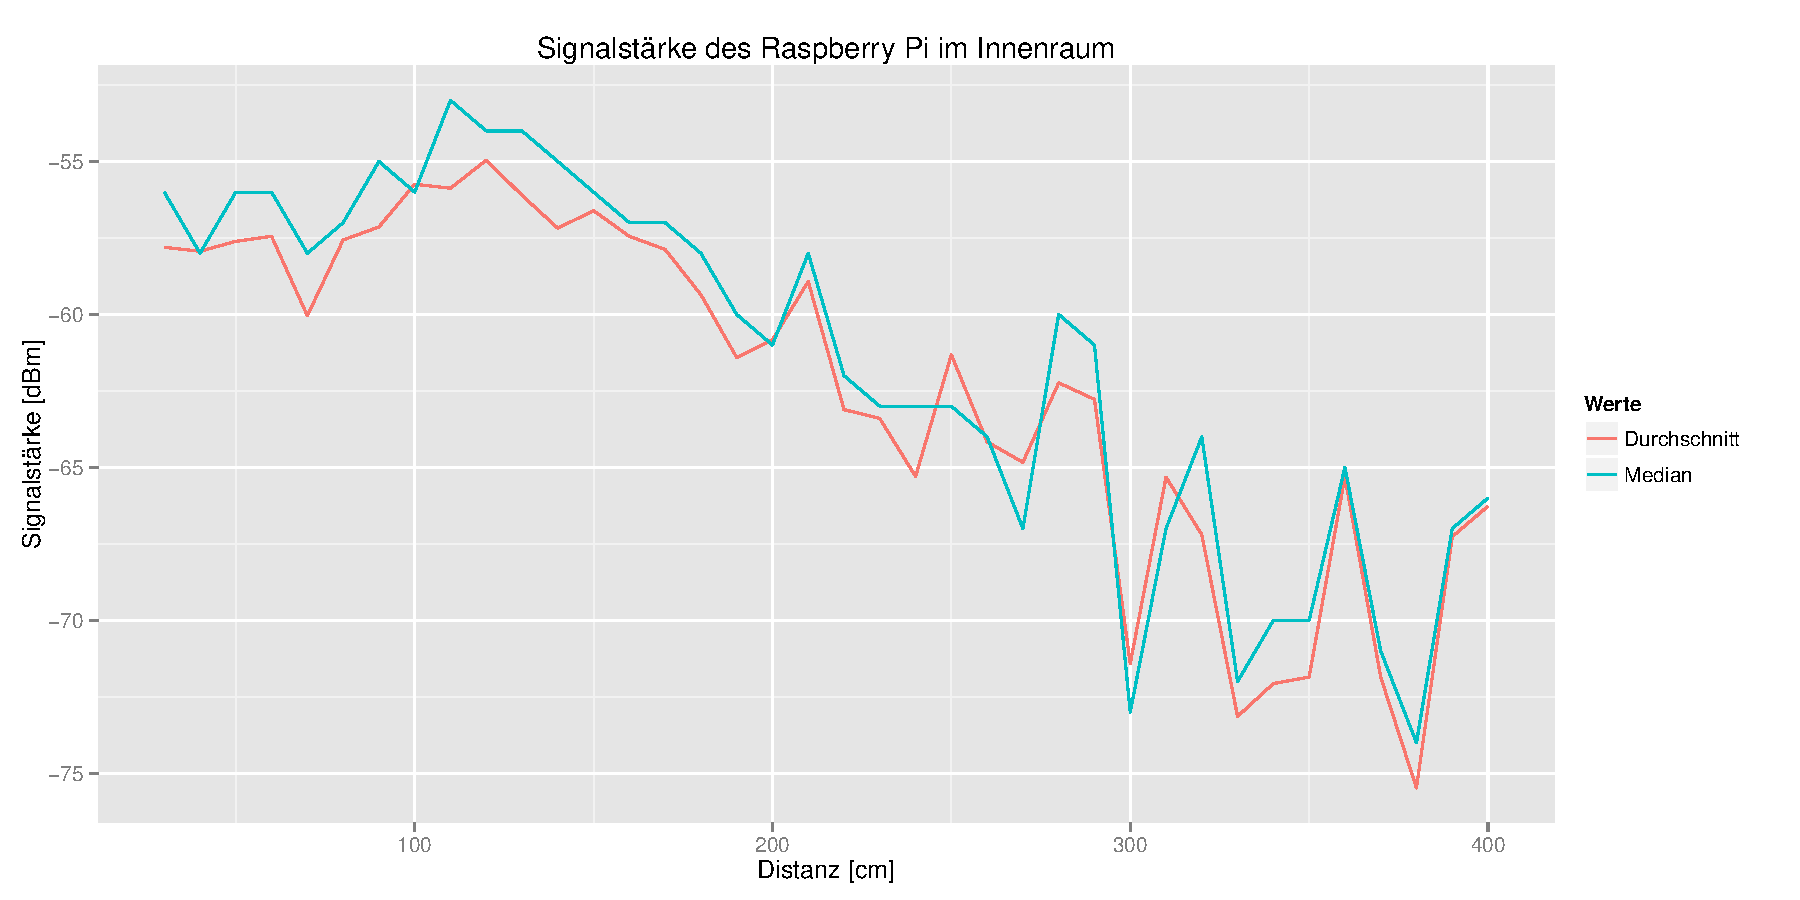
\includegraphics[scale=0.5]{avgmedianiphone5_raspberry}
	\caption{Vergleich zwischen dem arithmetischen Mittel und dem Median}
	\label{avgmedianiphone5_raspberry}
\end{figure}

Wie in Abbildung \ref{avgmedianiphone5_raspberry} zu erkennen, ist der Unterschied zwischen Median und arithmetischem Mittel jedoch zu vernachlässigen. 

%%%%%%%%%%%%%%%%%%%%%%%%%%%%%%%%%%%%%%%%%%%%%%%%%%%%%%%%%%%%
\subsubsection{Implementierung}
\label{sec:implementation:fingerprinting:positioning:avg:implementiation}
%%%%%%%%%%%%%%%%%%%%%%%%%%%%%%%%%%%%%%%%%%%%%%%%%%%%%%%%%%%%
Für die Implementierung der Positionsbestimmung mit Mittelwerten wird das CoreData-Modell um eine Entität namens \emph{BeaconInCell} erweitert. Diese Entität repräsentiert ein Beacon in einer bestimmten Zelle und wird zur Speicherung der Mittelwerte genutzt. Dadurch ist es nicht nötig die Mittelwerte für jede Positionsbestimmung neu zu berechnen, wobei über alle Fingerprints iteriert werden muss. Die Mittelwerte müssen so nur beim Hinzufügen neuer Fingerprints aktualisiert werden.

\textbf{BeaconInCell:}
	\begin{quote}Repräsentiert ein Beacon in einer bestimmten Zelle und beinhaltet durchschnittliche, maximale und minimale Signalstärke, sowie den Median der Signalstärke des Beacons in der aktuellen Zelle\end{quote}

Bei der Bestimmung der nächsten Zelle arbeitet dieses Verfahren quasi identisch zu dem vorherigen Nearest-Neighbor-Verfahren, doch statt über die Messungen zu iterieren, wird dabei über die Zellen iteriert. Dabei werden die Mittelwerte jeder Zelle mit den aktuell gemessenen Werten verglichen. Die Zelle mit dem geringsten euklidischen Abstand ist dabei die wahrscheinlichste Zelle der aktuellen Position.

%%%%%%%%%%%%%%%%%%%%%%%%%%%%%%%%%%%%%%%%%%%%%%%%%%%%%%%%%%%%
\subsection{Prohabilistisches Verfahren}
\label{sec:implementation:fingerprinting:positioning:probability}
%%%%%%%%%%%%%%%%%%%%%%%%%%%%%%%%%%%%%%%%%%%%%%%%%%%%%%%%%%%%

%%%%%%%%%%%%%%%%%%%%%%%%%%%%%%%%%%%%%%%%%%%%%%%%%%%%%%%%%%%%
\subsubsection{Algorithmus}
\label{sec:implementation:fingerprinting:positioning:probability:algorithm}
%%%%%%%%%%%%%%%%%%%%%%%%%%%%%%%%%%%%%%%%%%%%%%%%%%%%%%%%%%%%

Der letzte untersuchte Ansatz war ein prohabilistisches Verfahren, welches die Wahrscheinlichkeiten einer bestimmten Signalstärke eines Beacons als Referenz-Wert für die Positionbestimmung nutzt. Dabei wurde für die Berechnung der Wahrscheinlichkeiten und Bestimmung der aktuellen Position das Verfahren von \citet{wifiFingerprintProbability} verwendet, welche das Fingerprinting mit Hilfe von Wireless LAN-Routern verwenden.

Da das Fingerprinting mittels Wireless LAN ebenfalls auf den Signalstärken der Wireless LAN-Basisstationen basiert, lässt sich das Verfahren auch auf andere Technologien, welche die Signalstärke zur Positionsbestimmung nutzen, übertragen.

Während der initialen Offline-Phase wird, nachdem die Fingerprints gesammelt wurden, eine Wahrscheinlichkeitsverteilung der Signalstärken für jedes Beacon in jeder Zelle erstellt. Diese wird später als Vergleichswert genutzt, um die Ähnlichkeit der Signalstärken zu bestimmen.

\begin{figure}[htb!]
		\centering
	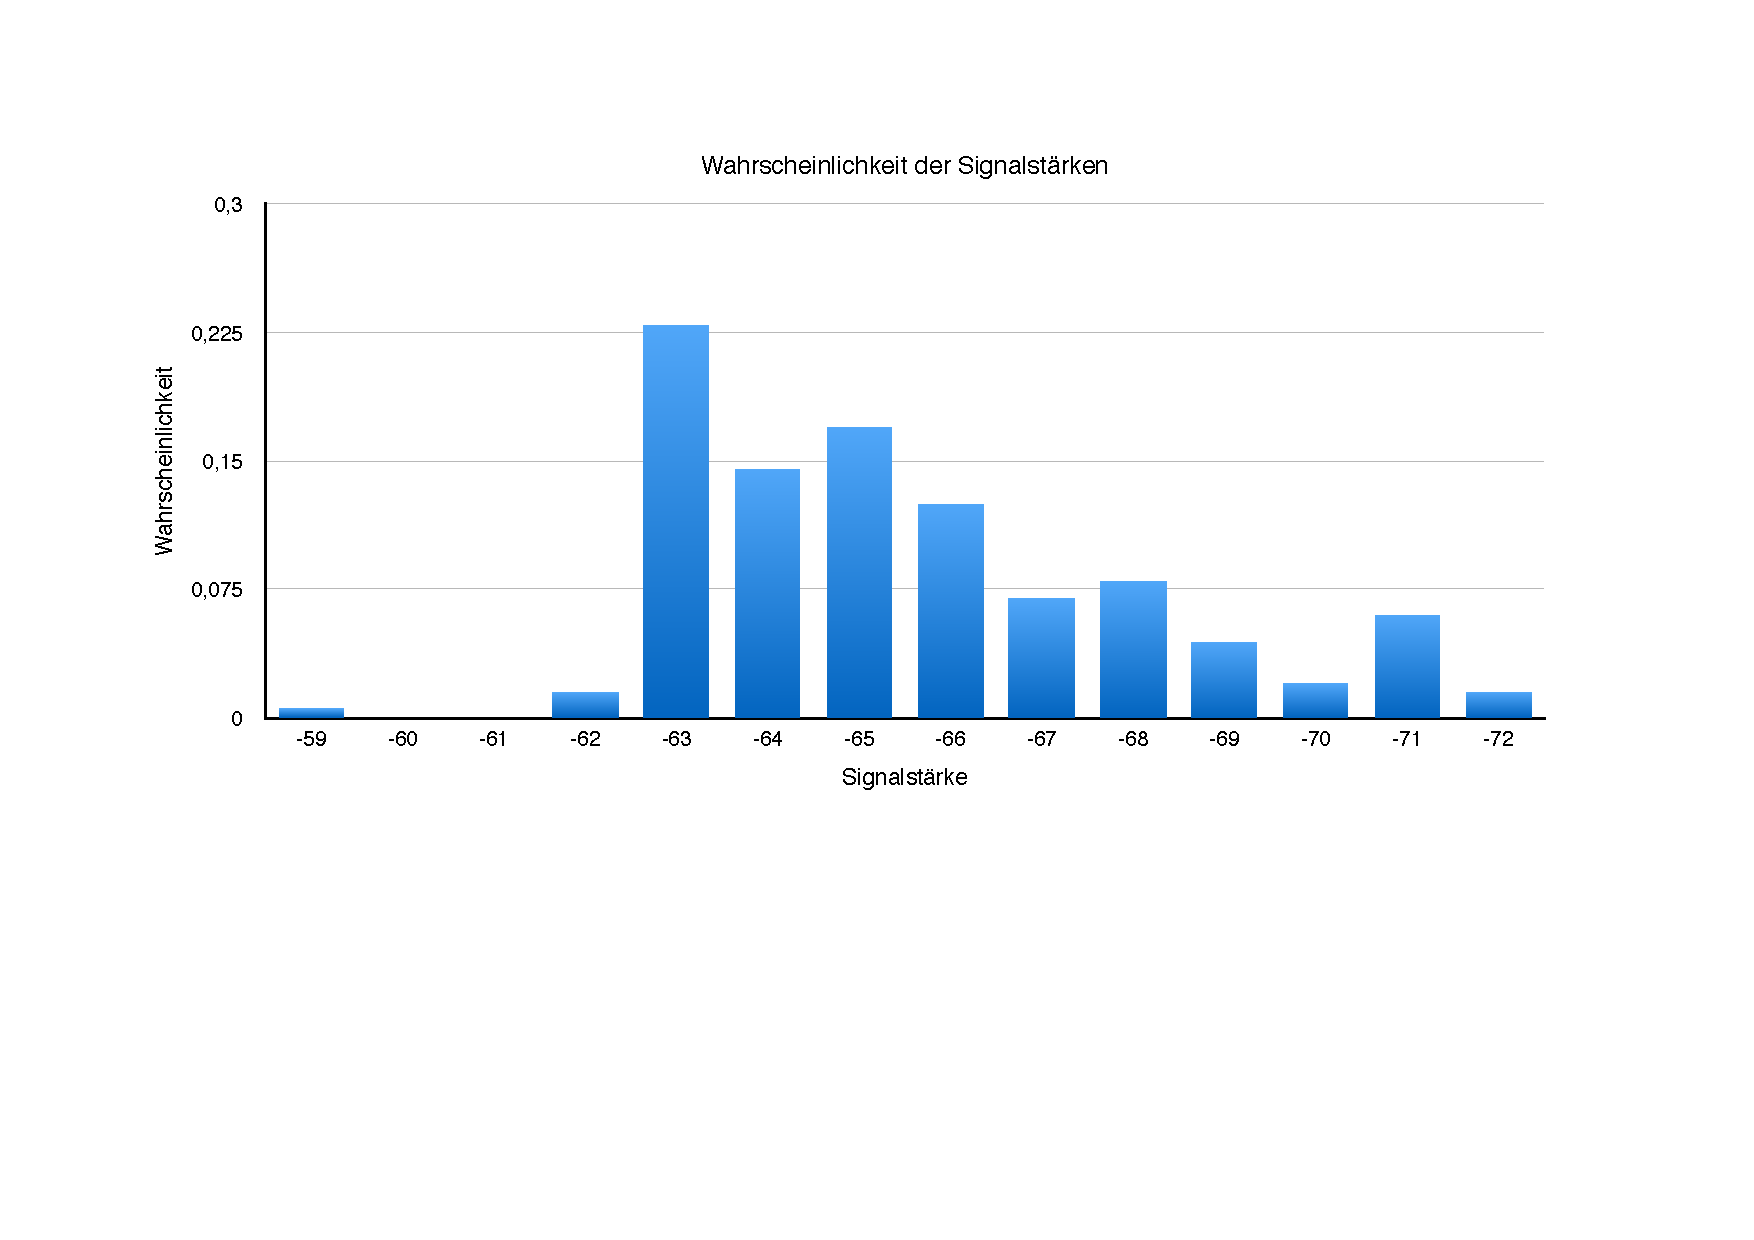
\includegraphics[scale=0.3]{probability_signal_strength}
	\caption{Wahrscheinlichkeitsverteilung von Signalstärke bei einem Beacon}
	\label{probability-signal-strength-beacon}
\end{figure}

Danach folgt die Online-Phase in der die aktuelle Position bestimmt werden soll. Dafür werden die aktuellen Signalstärken der Beacons gemessen und gespeichert, um von diesen Werten ebenfalls eine Wahrscheinlichkeitsverteilung zu berechnen. Die Anzahl der Werte, welche in die Wahrscheinlichkeitsverteilung einfließen ist dabei sehr wichtig.
Für eine statische Positionsbestimmung sollte die Anzahl der letzten gespeicherten Werte groß gewählt werden, da hier keine Echtzeit-Änderung der Position geschieht.
Für unsere Anwendung der Echtzeit-Positionsbestimmung ist ein relativ schnelles aktualisieren der Position jedoch essenziell. Daher muss hier ein Kompromiss aus akkurater Positionsbestimmung und Echtzeit-Fähigkeit gefunden werden.

Die Wahrscheinlichkeitsverteilung der aktuell gemessenen Werte muss nun mit den Verteilungen aller Zellen verglichen werden und deren Ähnlichkeit muss bestimmt werden. Dafür wird die Bhattacharyya-Distanz genutzt, welche die Ähnlichkeit zweier Wahrscheinlichkeitsverteilungen beschreibt. 
Diese Distanz muss für jede Zelle errechnet werden. 
Dafür muss zunächst der Bhattacharyya-Koeffizient $B_{b, c}$ für jedes Beacon $b$ einer Zelle $c$ berechnet werden.

\begin{equation}
	B_{b, c} = \sum_{s \in [s_{min},s_{max}]} \sqrt{P_{b}^{c}(s) \cdot Q_{b}(s)}
\end{equation}

Um daraus die Bhattacharyya-Distanz für die aktuelle Zelle $c$ zu berechnen, wird zunächst das arithmetische Mittel der Bhattacharyya-Koeffizienten der $q$ stärksten Beacons der aktuellen Zelle $O_{c}^{q}$ gebildet. Die Bhattacharyya-Distanz $d_{c}$ ist dabei der negative Logarithmus über diesen Mittelwert.

\begin{equation}
	d_{c}= \begin{cases}
	-ln (\frac{1}{q} \sum_{i \in O_{c}^{q}} B_{b, c}) & \text{wenn } \sum_{i \in O_{c}^{q}} B_{b, c} > 0 \\
	- \infty & \text{sonst}
	\end{cases}
\end{equation}

Diese Distanz gibt nun die Ähnlichkeit der aktuellen Wahrscheinlichkeitsverteilung mit den Wahrscheinlichkeitsverteilungen der jeweiligen Zelle an. Daraus ergibt sich, dass die Zelle mit der kleinsten Distanz die wahrscheinlichste Zelle für die aktuellen Messwerte ist.

Für unseren Zweck reicht diese Angabe aus. Es lässt sich jedoch, wie im Paper von \citet{wifiFingerprintProbability} weiter ausgeführt, auch noch eine interpolierte Position aus den $k$ wahrscheinlichsten Positionen bilden, welche, gewichtet nach ihrer Distanz, in die finale Position einfließen. Da wir jedoch mit Zellen arbeiten und nicht mit Koordinaten wurde darauf verzichtet. 

%%%%%%%%%%%%%%%%%%%%%%%%%%%%%%%%%%%%%%%%%%%%%%%%%%%%%%%%%%%%
\subsubsection{Implementierung}
\label{sec:implementation:fingerprinting:positioning:probability:implementiation}
%%%%%%%%%%%%%%%%%%%%%%%%%%%%%%%%%%%%%%%%%%%%%%%%%%%%%%%%%%%%
Für die Implementierung wurde das CoreData-Modell abermals erweitert, da eine neue Entität benötigt wird, welche die Wahrscheinlichkeitsverteilungen speichert. Dies geschieht aus dem gleichen Grund wie zuvor die Speicherung der Mittelwert, um die Rechenintensität während der Positionierungsphase gering zu halten.
Die neue Entität \emph{BeaconInCellProbability} hat dabei eine \emph{to-many} Beziehung zu der BeaconInCell-Entität. Die neue Entität besitzt zwei Attribute, die Signalstärke und deren Wahrscheinlichkeit. Jedes Beacon in einer Zelle hat dabei mehrere Wahrscheinlichkeitswerte.
\todo{Darstellung der Dateistruktur in CoreData}


%%%%%%%%%%%%%%%%%%%%%%%%%%%%%%%%%%%%%%%%%%%%%%%%%%%%%%%%%%%%
\section{Anzeige auf der Karte}
\label{sec:implementation:map}
%%%%%%%%%%%%%%%%%%%%%%%%%%%%%%%%%%%%%%%%%%%%%%%%%%%%%%%%%%%%
Wie bereits erwähnt, wird für die Anzeige der aktuellen Position auf der Karte ein externes Framework von MapBox genutzt.
Dieses muss zunächst in das Projekt eingebunden werden. 
Nach dem Einbinden können die vom Framework bereitgestellten Klassen und Funktionen genutzt werden.
Für die Anzeige auf dem Gerät ist es zunächst nötig einen \emph{RMMapView} anzulegen, welcher für die Ausgabe der Karte verantwortlich ist und gleichzeitig die gewohnten MapView-Features wie zum Beispiel \emph{Pinch-to-Zoom} oder die automatische Ausrichtung auf den Mittelpunkt mit sich bringt.
Da wir unser eigenes Kartenmaterial verwendet ist es zudem nötig die Quelle für Kartendaten des MapViews zu ändern, da ansonsten die Daten des OpenStreetMap-Projekts genutzt werden.
Dazu muss zunächst die generierte \emph{mbtiles} Datei in die Verzeichnisstruktur des Projektes aufgenommen werden. Dafür wird ein Ordner namens \emph{Supporting Files} bereitgestellt. Durch das Zufügen der Datei wird auch der spätere Offlinebetrieb möglich, da diese lokal auf dem Endgerät gespeichert wird.
Um diese Datei als Grundlage für die spätere Karte zu verwenden, wird ein neues \emph{RMTileSource}-Objekt angelegt, welche mit der \emph{mbtiles}-Datei initialisiert wird. Daraufhin muss diese neue Kartenquelle als genutzte Kartenquelle für den \emph{RMMapView} gesetzt werden.
  
In Listing \ref{lst:RMMapView_objc} wird diese Initialisierung gezeigt.
\begin{listing}[htb!]
    \insertminted{objc}{code_examples/RMMapView.m}
    \caption{Initialisierung des MapView mit eigenem Kartenmaterial}
	\label{lst:RMMapView_objc}
\end{listing}

Nachdem die Karte initialisiert wurde, muss nun die aktuelle Position auf der Karte gezeigt werden. Dazu müssen die Zellennummer in die Kartenkoordinaten überführt werden. Nachdem das geschehen ist, lässt sich eine \emph{RMAnnotation} auf der Karte anzeigen, welche die aktuelle Position im Raum widerspiegelt.
\chapter{Versuchsergebnisse}
\label{chap:testing}

Im Anschluss an die Implementierung der verschiedenen Algorithmen, sollten diese unter realen Bedingungen getestet werden. 
Dazu wurde ein Versuchsaufbau innerhalb eines Gebäudes aufgebaut, welches aus mehreren Räumen besteht. Dafür werden 9 Beacons innerhalb des Gebäudes verteilt. 
In der Offline-Phase werden dabei für jede Position 40 Fingerprints gesammelt, jeweils 10 in 90 Grad gedrehten Ausrichtungen.

Untersucht werden soll dabei zum einen die Genauigkeit der Positionierung eines sich bewegenden Objektes. Hierfür wird der Pfad aufgezeichnet und mit dem realen Pfad verglichen.
Zum Anderen soll die Positionierung an einer statischen Position getestet werden. Dazu wird an verschiedenen Testpunkten geprüft, ob die ausgegebene Position mit der realen Position übereinstimmt.

Der Testraum besteht dabei aus drei benachbarten Zimmern, wobei zwei dieser Zimmer durch ein offenen Durchgang verbunden sind. Das andere Zimmer ist über eine Tür zu erreichen. 
In Abbildung \ref{messraum} lässt sich der Aufbau des Messraumes erkennen, wobei die Dreiecke die eingemessenen Positionen darstellen und die Beacons als blaue Antennen gezeigt werden.

\begin{figure}[htb!]
		\centering
	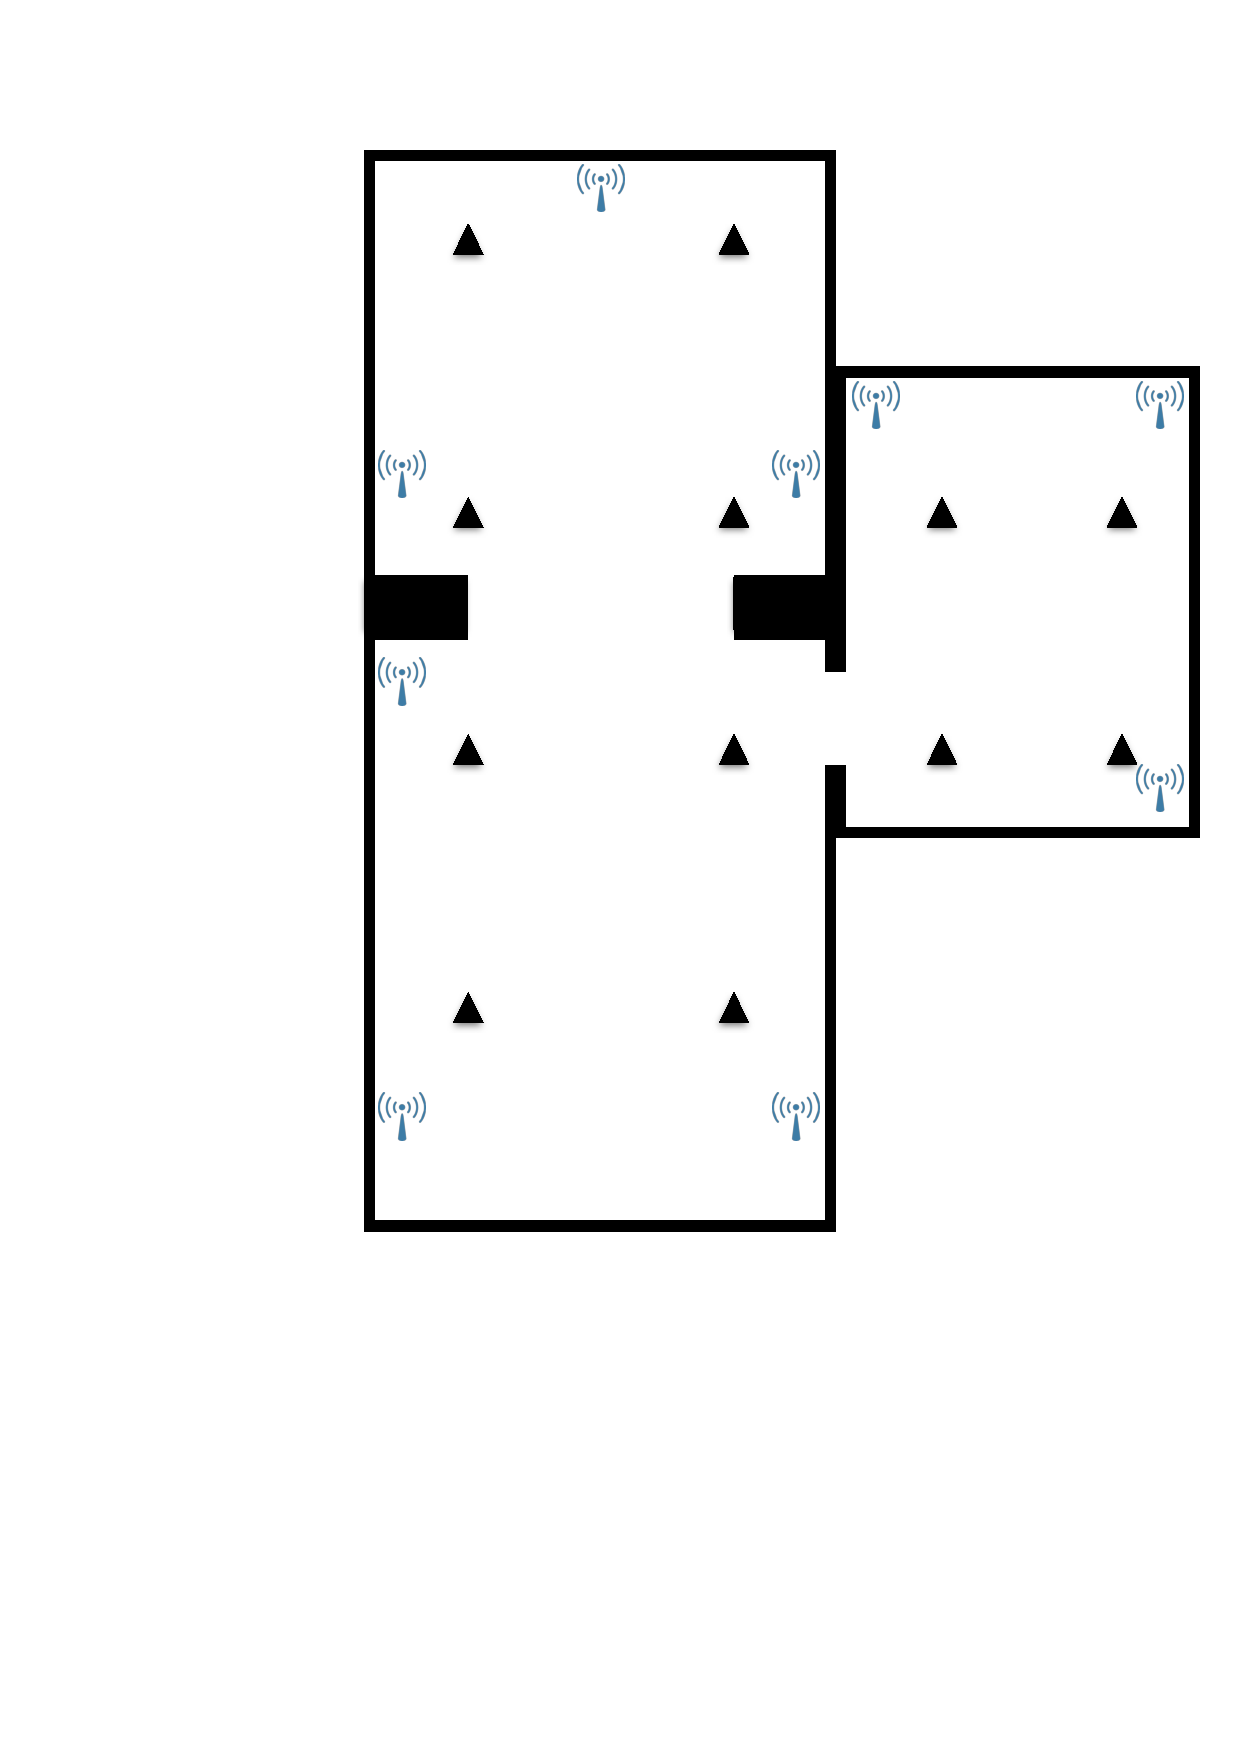
\includegraphics[scale=0.5]{messraum}
	\caption{Abbildung der Messraumes}
	\label{messraum}
\end{figure}

Die Abstände zwischen den einzelnen Messpositionen betragen dabei zwei Meter, woraus sich auch die mögliche Genauigkeit der Messung ergibt.

%%%%%%%%%%%%%%%%%%%%%%%%%%%%%%%%%%%%%%%%%%%%%%%%%%%%%%%%%%%%
\section{Positionierung eines beweglichen Objektes}
\label{sec:testing:moving}
%%%%%%%%%%%%%%%%%%%%%%%%%%%%%%%%%%%%%%%%%%%%%%%%%%%%%%%%%%%%

Bei den Tests der Positionierung bei einem bewegenden Objekt wird zuerst ein abzulaufender Pfad festgelegt, welcher jeweils über die Mittelpunkte der zuvor eingemessenen Zellen führt. Dieser Pfad wird dabei langsam abgelaufen und die Positionierungsangabe für jeden Algorithmus werden aufgezeichnet und nach Beendigung der Messungen wird der gemessene Pfad mit dem realen Pfad verglichen. Dabei wird das Hauptaugenmerk auf die Korrektheit der Position, die Größe der Abweichung und die Echtzeitfähigkeit des verwendeten Algorithmus gelegt.

Bei der Durchführung wurde zwei vorgegebene Wege abgelaufen. Bei der Analyse wird dabei der real abgeschrittene Weg mit dem, durch die Algorithmen errechneten, Weg verglichen.

Alle getesteten Algorithmen unterlagen dabei relativ starken Schwankungen zwischen einzelnen Zelle. Das Verfahren mittels Wahrscheinlichkeitsverteilungen erreichte bei diesem Test die höchste Genauigkeit, wobei hier die errechnete Position immer wieder zwischen der Zelle der aktuellen Position und den benachbarten Zellen wechselte. Durch diese Ungenauigkeit war es daher nicht möglich den genauen Laufweg zu reproduzieren. Eine Aussage darüber, in welchem Raum sich das Gerät aktuell befindet, konnte jedoch mit sehr großer Sicherheit durchgeführt werden.

Auch das Nearest-Neighbor-Verfahren über die gesamte Fingerprintdatenbank erlaubte ähnliche Aussagen zu treffen, obwohl es etwas instabiler als das probabilistische Verfahren ist. Der Vorteil dieses Systems ist die schnellere Aktualisierungsrate, da es nur auf den letzten gemessenen Wert zurückgreift. Das probabilistische Verfahren hingegen nutzt die letzten fünf gemessenen Werte, wodurch sich die Aktualisierung der Position um einige Sekunden verzögert.

Das Nearest-Neighbor-Verfahren über die Mittelwert schnitt bei dieser Untersuchung schlecht ab. Eine Positionsangabe war kaum möglich, da die Zellenangaben stark schwankten und im Großteil der Fälle ein falsche Position anzeigt wurde.


Bei der Positionierung von beweglichen Objekten ist der probabilistische Algorithmus am Besten geeignet, da dieser einen guten Kompromiss zwischen Genauigkeit und Aktualisierungsrate bietet. Falls mehr Wert auf eine sehr schnell Aktualisierung gelegt wird, sollte jedoch der Nearest-Neighbor-Algorithmus über alle Fingerprints genutzt werden, da dieser eine sofortige Aktualiserung der Position mit sich bringt.

%%%%%%%%%%%%%%%%%%%%%%%%%%%%%%%%%%%%%%%%%%%%%%%%%%%%%%%%%%%%
\section{Statische Positionierung}
\label{sec:testing:static}
%%%%%%%%%%%%%%%%%%%%%%%%%%%%%%%%%%%%%%%%%%%%%%%%%%%%%%%%%%%%

Bei der statischen Positionierung wird an verschiedenen festen Positionen eine Positionsmessung durchgeführt. Dabei werden die Ergebnisse der verschiedenen Algorithmen verglichen. Es wird neben der korrekten Positionsangabe besonders auf die Konstanz dieser Positionsangabe geachtet. Diese sollte nicht zu stark schwanken und sich nach kurzer Zeit auf die korrekte Position einpendeln.

Bei der Untersuchung der statischen Positionierung wurde an vier verschiedenen Punkten im Messraum für 20 Sekunden Stichproben genommen. Dabei wurden alle implementierten Algorithmen untersucht und direkt verglichen.

Es wird eine grobe Unterteilung genutzt, sodass eine Positionierung entweder die richtige Zelle bestimmt, eine benachbarte Zelle oder eine weiter entfernte Zelle als aktuelle Position angibt. 

Wie bereits erwartet, schnitt der Algorithmus mit der Wahrscheinlichkeitsverteilung am Besten ab. Dieser schaffte es in knapp zwei Drittel der Fälle die genaue Position zu bestimmen. In den restlichen Fällen bestimmte der Algorithmus eine benachbarte Position als aktuelle Position. Dabei wurde kein Mal eine nicht in unmittelbarer Nachbarschaft befindliche Position als aktuelle Zelle angenommen. 

Überraschender Weise liegt der Nearest-Neighbor-Algorithmus, welcher über alle Fingerprints iteriert, von der Genauigkeit an der zweiten Stelle. Die Quote der richtigen Positionsangaben lag dabei bei etwa 50 Prozent. In etwa 40 Prozent der Fälle wurde eine benachbarte Position als die aktuelle Position bestimmt und nur in einem Zehntel der Fälle wurde eine Position, welche sich nicht in der direkten Nachbarschaft befindet, bestimmt.
Der Nearest-Neighbor-Algorithmus mit dem Median und der durchschnittlichen Signalstärke lagen bei der Messung gleich auf. Dabei ergab sich bei dieser Methode nur eine Treffrate von 36 Prozent. Als benachbarte Zelle werden nur etwa 5 Prozent der erkannten Positionen bestimmt. Die Fehlerquote dieser Methode liegt dabei bei über der Hälfte aller bestimmten Positionen und ist so nicht ausreichend genau.

% \begin{tabular}{lcr}
%   & Nearest-Neighbor für alle Fingerprint & Nearest-Neighbor für Median und Durchschnittswerte & Wahrscheinlichkeitsmethode \\
%   Genaue Zelle & 51,3 & 36,8 & 68,4 \\
%   Benachbarte Zelle & 39,5 & 52,6 & 31,6 \\
%   Entfernte Zelle & 9,2 & 57,9 & 0 \\
% \end{tabular}
\begin{figure}[htb!]
		\centering
	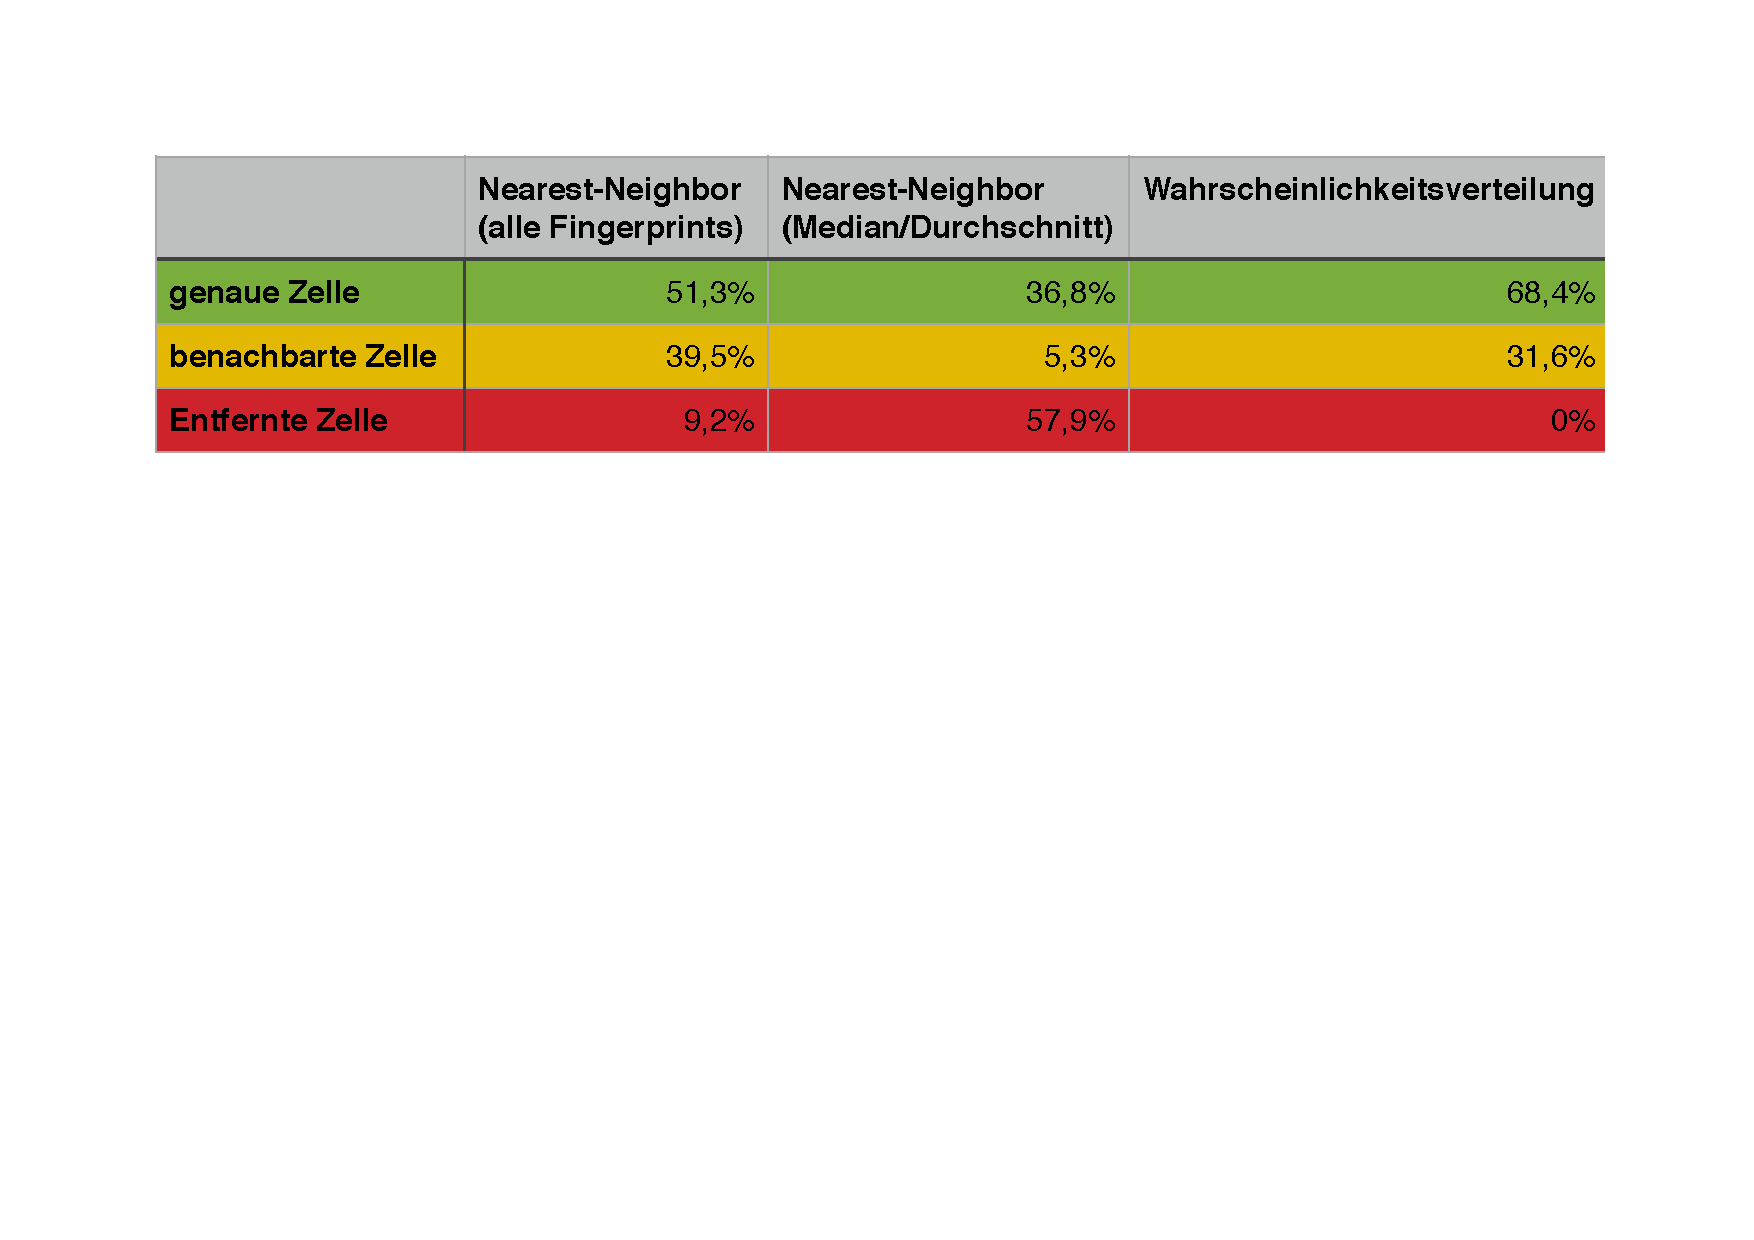
\includegraphics[scale=0.5]{statistic-static}
	\caption{Genauigkeitswerte der statischen Lokalisierung}
	\label{statistic-static}
	\end{figure}
 
Für eine statische Positionierung ist das Verfahren zur Positionierung mittels Wahrscheinlichkeitsverteilungen sehr gut geeignet. Die Genauigkeit ist dabei ausreichend, da der größte gemessene Fehler eine Lokalisierung in eine benachbarten Zelle ist. Außerdem ist dieses Verfahren relativ robust und es sind nur geringe Schwankungen in der Positionierung zu beobachten.

Auch das Nearest-Neighbor-Verfahren über die gesammte Datenbank der Fingerprints liefert akzeptable Ergebnisse und liegt nur in unter 10 Prozent der Fälle außerhalb der eigentlichen oder benachbarten Zelle. Hierbei sind jedoch schon größere Schwankungen zu erkennen, sodass die Positionierung häufiger zwischen zwei oder mehreren Zelle springt.

Die Nearest-Neighbor-Methode mit den Mittelwerte ist weniger geeignet für die Indoor Positionierung, da hier eine sehr hohe Fehlerrate vorliegt und die Ergebnisse zudem sehr stark schwanken.
\chapter{Fazit und Ausblick}
\label{chap:resume}

%\include{kapitel/state_of_the_art}
%\include{kapitel/performance_investigation}
%\include{kapitel/example_application}
%\include{kapitel/reflexion}

%%%%%%%%%%%%%%%%%%%%%%%%%%%%%%%%%%%%%%%%%%%%%%%%%%%%%%%%%%%%%
%% einleitung.tex
%%
%% Kapitel: Einleitung
%% Hauptdokument: howto.tex
%% Autor: Tobias Luksch
%% Datum: Juli 2003
%%%%%%%%%%%%%%%%%%%%%%%%%%%%%%%%%%%%%%%%%%%%%%%%%%%%%%%%%%%%
\chapter{Einleitung}
\label{chap:einl}

%%%%%%%%%%%%%%%%%%%%%%%%%%%%%%%%%%%%%%%%%%%%%%%%%%%%%%%%%%%%
\section{Motivation}
\label{sec:einl:motiv}
%%%%%%%%%%%%%%%%%%%%%%%%%%%%%%%%%%%%%%%%%%%%%%%%%%%%%%%%%%%%
Die Arbeitsgruppe Technische Informatik an der
Universit�t Osnabr�ck bietet eine Vielzahl von Angeboten an
studentischen Arbeiten an, seien es Abschlussarbeiten,
Seminare oder Praktika. F�r all diese Arbeiten ist ein Dokument zu
erstellen, das die Anspr�che an eine wissenschaftliche Arbeit erf�llen
sollte. Um es den Studierenden einfacher zu machen, diesen Anspr�chen
gerecht zu werden, bietet die Arbeitsgruppe \LaTeX -Vorlagen an,
die ein professionelles und einheitliches Layout erm�glichen.
% Diese Dokumentation 
% beschreibt die Formatvorlage f�r \emph{Abschlussarbeiten}.

%%%%%%%%%%%%%%%%%%%%%%%%%%%%%%%%%%%%%%%%%%%%%%%%%%%%%%%%%%%%
\section{Ziel der Arbeit}
\label{sec:einl:ziel}
%%%%%%%%%%%%%%%%%%%%%%%%%%%%%%%%%%%%%%%%%%%%%%%%%%%%%%%%%%%%
Das Ziel dieser Dokumentation ist es, Studierenden eine Anleitung zum
Erstellen wissenschatlicher Dokumente an die Hand zu geben. Dabei wird
auf Besonderheiten der zur Verf�gung gestellen \LaTeX -Klasse ebenso
eingegangen wie auf einige prinzipelle Formalismen wissenschatlicher
Arbeiten. Es wird aufgezeigt, wie Bilder oder Tabellen korrekt
erstellt und referenziert werden und wie ein Literaturverzeichnis
erstellt wird. Dieses Dokument selbst dient als Beispiel und kann als
Vorlage und Ausgangspunkt f�r eigene Arbeiten verwendet werden.

Es sei angemerkt, dass dies weder eine Einf�hrung in \LaTeX\ ist, noch wird
eine Anleitung zur Installation von \LaTeX -Distributionen gegeben.
Dazu sei deshalb auf die einschl�gige Literatur (zum Beispiel
\cite{Lamport95}, \cite{Goossens96}) oder Webseiten (\cite{WWWDante},
\cite{WWWMikTex}) verwiesen.

Weiterhin sei bemerkt, dass der Sprachstil dieser Arbeit �ber weite
Teile (nicht �berall) formaler gehalten ist als notwendig.
Der Grund hierf�r liegt in der Intention, dem Leser einen Eindruck zu
vermitteln, welcher Art der Stil einer wissenschaftlichen Arbeit sein
sollte. Man m�ge dem Autor deshalb den Mangel an Lockerheit und
humoristischen Ausschweifungen verzeihen.

% %%%%%%%%%%%%%%%%%%%%%%%%%%%%%%%%%%%%%%%%%%%%%%%%%%%%%%%%%%%%
% \section{Aufbau der Arbeit}
% \label{sec:einl:aufbau}
% Kapitel~\ref{chap:klasse} besch�ftigt sich zun�chst mit der von der AG
% Robotersysteme angebotenen \LaTeX -Klasse \latexklasse. Es wird
% erl�utert, welche Form das Hauptdokument haben muss und welche Makros
% zur Verf�gung gestellt werden.
% 
% Anschlie�end finden sich in Kapitel~\ref{chap:floats} Anleitungen zum
% Erstellen besonderer Dokumentelemente. Bilder und Tabellen werden
% ebenso behandelt wie Formeln oder Literaturverweise.
% 
% In Kapitel~\ref{chap:aufbau} werden einige kurze Hinweise zum
% allgemeinen Aufbau einer wissenschaftlichen Arbeit gegeben. Dies ist
% nur als Anregung zu verstehen, eine ausgiebige Einf�hrung hierzu w�rde
% den Rahmen dieser Dokumentation sprengen.


%%% Local Variables: 
%%% mode: latex
%%% TeX-master: "howto"
%%% End: 

%\input{kapitel/methoden_und_technologien}
%\input{kapitel/umsetzung_der_beispielapplikation}
%\input{kapitel/fazit}

% Dieser Stil erzeugt Verweise mit Autorenname und Jahr
%\bibliographystyle{gerapali}
%\bibliographystyle{abbrvnat}
\bibliographystyle{unsrt}
%\bibliographystyle{AGTI}
\addcontentsline{toc}{chapter}{Literaturverzeichnis}

% Hier die Datei (ohne .bib) angeben, in der die referenzierten
% Paper stehen
\bibliography{literatur}
%\clearpage{\cleardoublepage}
\clearpage

\appendix
\chapter{Glossar und Abkürzungsverzeichnis}

% \begin{tabular}{l}
% 	iBeacon / Beacon & Bluetooth-Sendegerät, welches kontinuierliche Identifizierungsinformationen sendet. Das Protokoll wurde von der Apple Inc. erstellt.  \\
% 	Location-based services & Dienste, welche abhängig vom aktuellen Aufenthaltsort bereitgestellt werden \\
% \end{tabular}

\begin{tabular}[t]{lp{10cm}}
	\textbf{Model-View-Controller} & Programmierkonzept für die Strukturierung des Programmmodels in drei Bereiche Model, View und Controller. \\ \\
	\textbf{Model} & Das Model enthält die darzustellenden Daten und ist komplett unabhängig von View und Controller. \\ \\
	\textbf{View} & Der View ist für die Anzeige der Daten und für die Entgegennahme von Nutzerinteraktionen verantwortlich. \\ \\
	\textbf{Controller} & Der Controller dient als Schnittstelle zwischen View und Model. Er wertet die Nutzerinteraktionen aus und reagiert diesen entsprechend. \\ \\
	\textbf{Segue} & Englisch für Übergang. Steuert in iOS-Applikationen den Wechsel zwischen zwei Views. \\ \\
	\textbf{ViewController} & Bezeichnung für den Controller eines Views in iOS \\ \\
	\textbf{Property} & Properties sind ähnlich den Instanzvariablen, bieten jedoch zusätzliche Zugriffssteuerung. Außerdem werden automatisiert Getter und Setter für ein Property erzeugt. \\ \\
    \textbf{iBeacon / Beacon} & Bluetooth-Sendestation, welche kontinuierlich Identifizierungsinformationen sendet. Das Protokoll wurde von Apple Inc. erstellt. \\ \\
    %\textbf{Entität} &  \\ \\
	\textbf{UUID} & Der Universally Unique Identifier ist ein standardisierter Identifikator, welche in der Softwareentwicklung genutzt wird. \\ \\
	\textbf{Delegate} & Delegates werden genutzt, um es Objekten einer Klasse zu ermöglichen mit dieser zu kommunizieren. Dazu muss die Klasse die entsprechenden Delegate-Methoden implementieren. \\ \\
 
 \end{tabular}
  
  \begin{tabular}[t]{lp{10cm}}
	\textbf{Nearest-Neighbor} & Der Nearest-Neighbor (Nächste-Nachbar) eines Werte ist ein Wert, welcher die geringste Distanz zu diesem aufweist. Dabei ist die Distanzfunktion frei wählbar. \\ \\
	\textbf{Fingerprint} & Ein Fingerprint ist ein Messwert an einer bestimmten Position, welcher eine Identifizierungsinformation und die Signalstärke für umliegende drahtlose Sendestationen beinhaltet.\\ \\
  	\textbf{Location-based service} & Als Location-based service bezeichnet man Dienste, welche von der aktuellen Position des Nutzers abhängig sind. \\ \\
  \end{tabular}
  
  
\chapter{Anleitung zur Nutzung der Applikation}

Die Applikation liegt in Quellcodeform auf der beiliegenden CD-ROM vor. Da Apple keine Installationen außerhalb des eigenen AppStores erlaubt, muss das Programm in Xcode kompiliert werden. Um die Applikation auf ein Gerät zu übertragen, ist eine Mitgliedschaft im Apple Developer Program nötig.

Die Applikation ist standardmäßig auf die Daten der kontakt.io Beacons eingestellt. Dabei kommt die UUID \emph{A41B74DE-F54E-411F-9F03-75D5253528A0} zum Einsatz. Falls andere Beacons zum Einsatz kommen, muss deren UUID entsprechend angepasst werden. 

Die Applikation an sich besteht aus drei grundlegenden Views, welche sich über die Tab-Bar im unteren Bereich des Bildschirmes erreichen lassen. 

Das Tab \emph{Collecting} erlaubt dabei die Sammlung der Fingerprintdaten. Dazu ist zunächst die Eingabe der aktuellen Zelle und der Anzahl der zu sammelnden Fingerprints einzugeben. Um den Sammelvorgang zu starten muss der Button \emph{Start Collecting Fingerprints} gedrückt werden. Die Vorgang wird danach automatisch gestartet und sobald die gewünschte Anzahl an Fingerprints gesammelt wurde, kehrt die Applikation zum vorherigen Bildschirm zurück. 
Bei der Sammlung der Fingerprints sollte die aktuelle Position nicht zu stark verändert werden, da dies negative Auswirkungen auf die Qualität der Fingerprints haben könnte.

Das Tab \emph{Information} erlaubt das Betrachten der bereits gesammelten Fingerprints. Dabei werden in einem TableView die bisher eingemessenen Zellen angezeigt. Bei einem Klick auf die jeweilige Zelle werden zusätzliche Informationen zu den Beacon in der Zelle angezeigt.

Das Tab \emph{Positioning} ist für die Lokalisierung zuständig. Nachdem verschiedene Zellen eingemessen wurde, ist es hier möglich die aktuelle Zelle anzuzeigen.
Dabei werden die Ergebnisse der verschiedenen Algorithmen untereinander angezeigt. 
Auch eine Karte wird eingeblendet, diese muss jedoch abhängig vom aktuellen Ort im Quellcode initialisiert werden. Daher ist die Positionsanzeige auf der Karte deaktiviert.

\cleardoublepage

  \vspace*{15cm}

  \chapter*{Erklärung}

  \thispagestyle{empty}

  Ich versichere, dass ich die eingereichte Bachelor-Arbeit selbstständig und ohne
  unerlaubte Hilfe verfasst habe. Anderer als der von mir angegebenen Hilfsmittel und
  Schriften habe ich mich nicht bedient. Alle wörtlich oder sinngemäß den Schriften
  anderer Autoren entnommenen Stellen habe ich kenntlich gemacht.

  \bigskip\bigskip

\begin{flushright}
Osnabrück, den 25.03.2014
\end{flushright}
\vskip 0.5 cm

 \bigskip
 \bigskip
 \bigskip
 \bigskip
 \bigskip

 (Kevin Seidel)


\end{document}
%%%%%%%%%%%%%%%%%%%%%%%%%%%%%%%%%%%%%%%%%%%%%%%%%%%%%%%%%%%%
%% Ende des Dokuments
%%%%%%%%%%%%%%%%%%%%%%%%%%%%%%%%%%%%%%%%%%%%%%%%%%%%%%%%%%%%
